\newcommand{\dnnfigurespostfit}{
\begin{figure}[h]
    \centering
    \subfloat[$\mjj$]{
        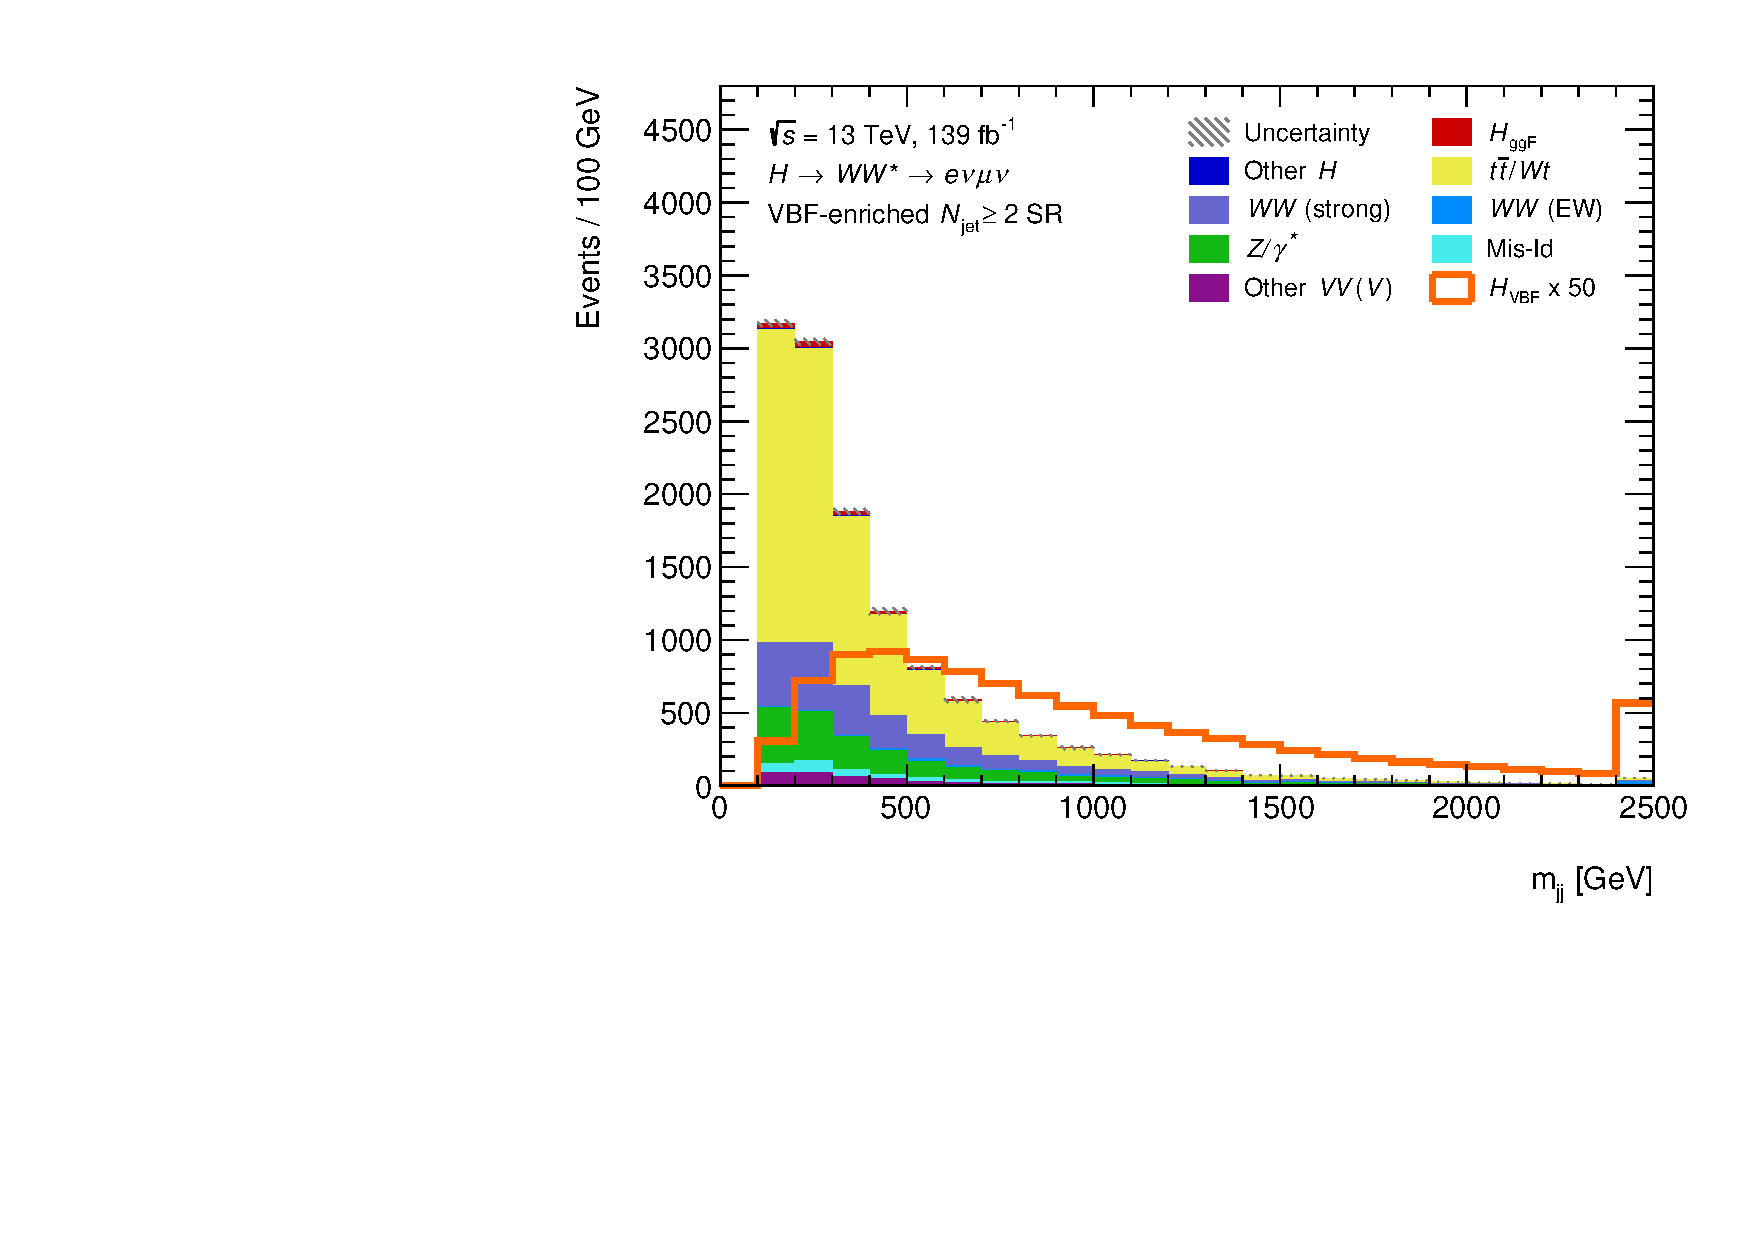
\includegraphics[width=0.32\textwidth]{figures/hww/dnn/blinded/run2-emme-CutVBF_SR-Mjj-lin.pdf} \hfill
        \label{fig:dnn-inputs-post-fit-1}
    } 
    \subfloat[$\dyjj$]{
        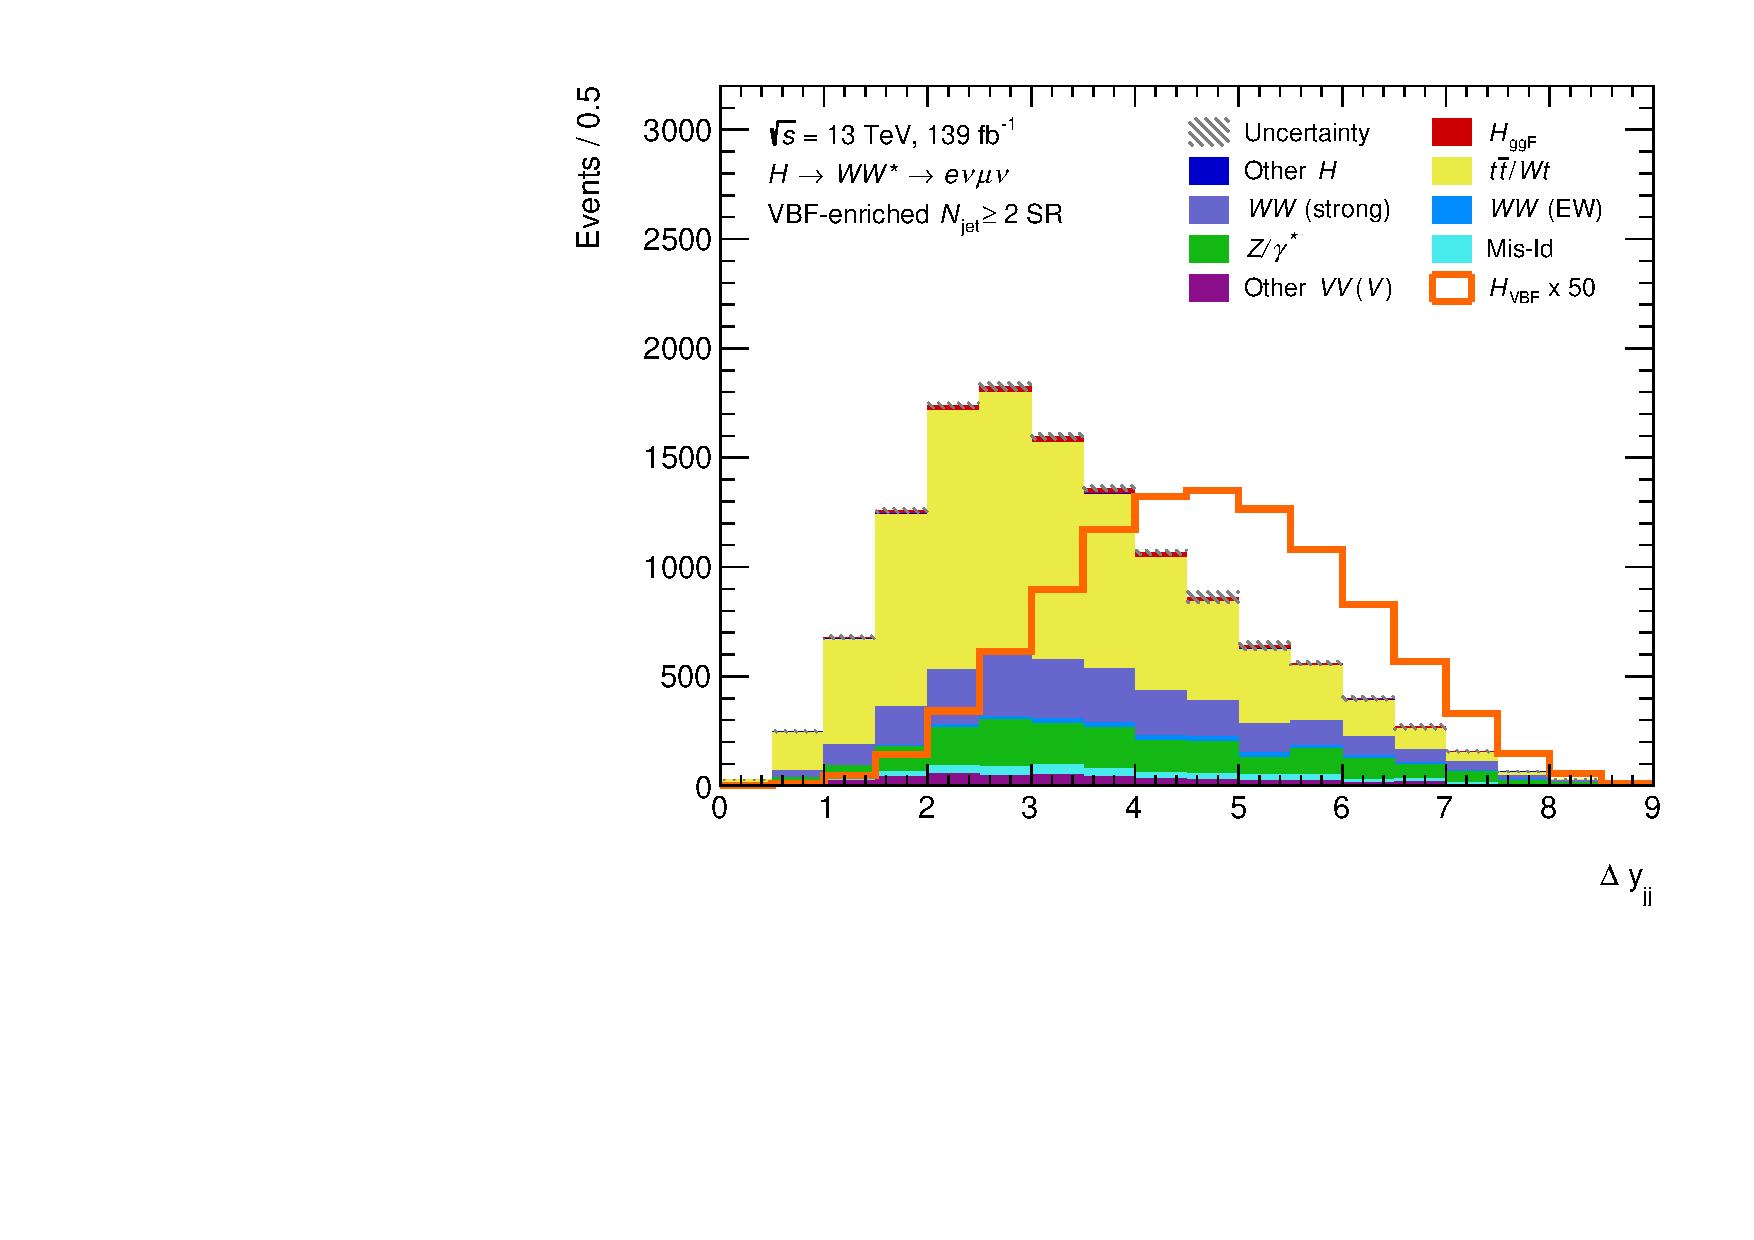
\includegraphics[width=0.32\textwidth]{figures/hww/dnn/blinded/run2-emme-CutVBF_SR-DYjj-lin.pdf} \hfill
        \label{fig:dnn-inputs-post-fit-2}
    } 
    \subfloat[$\lepetacent$]{
        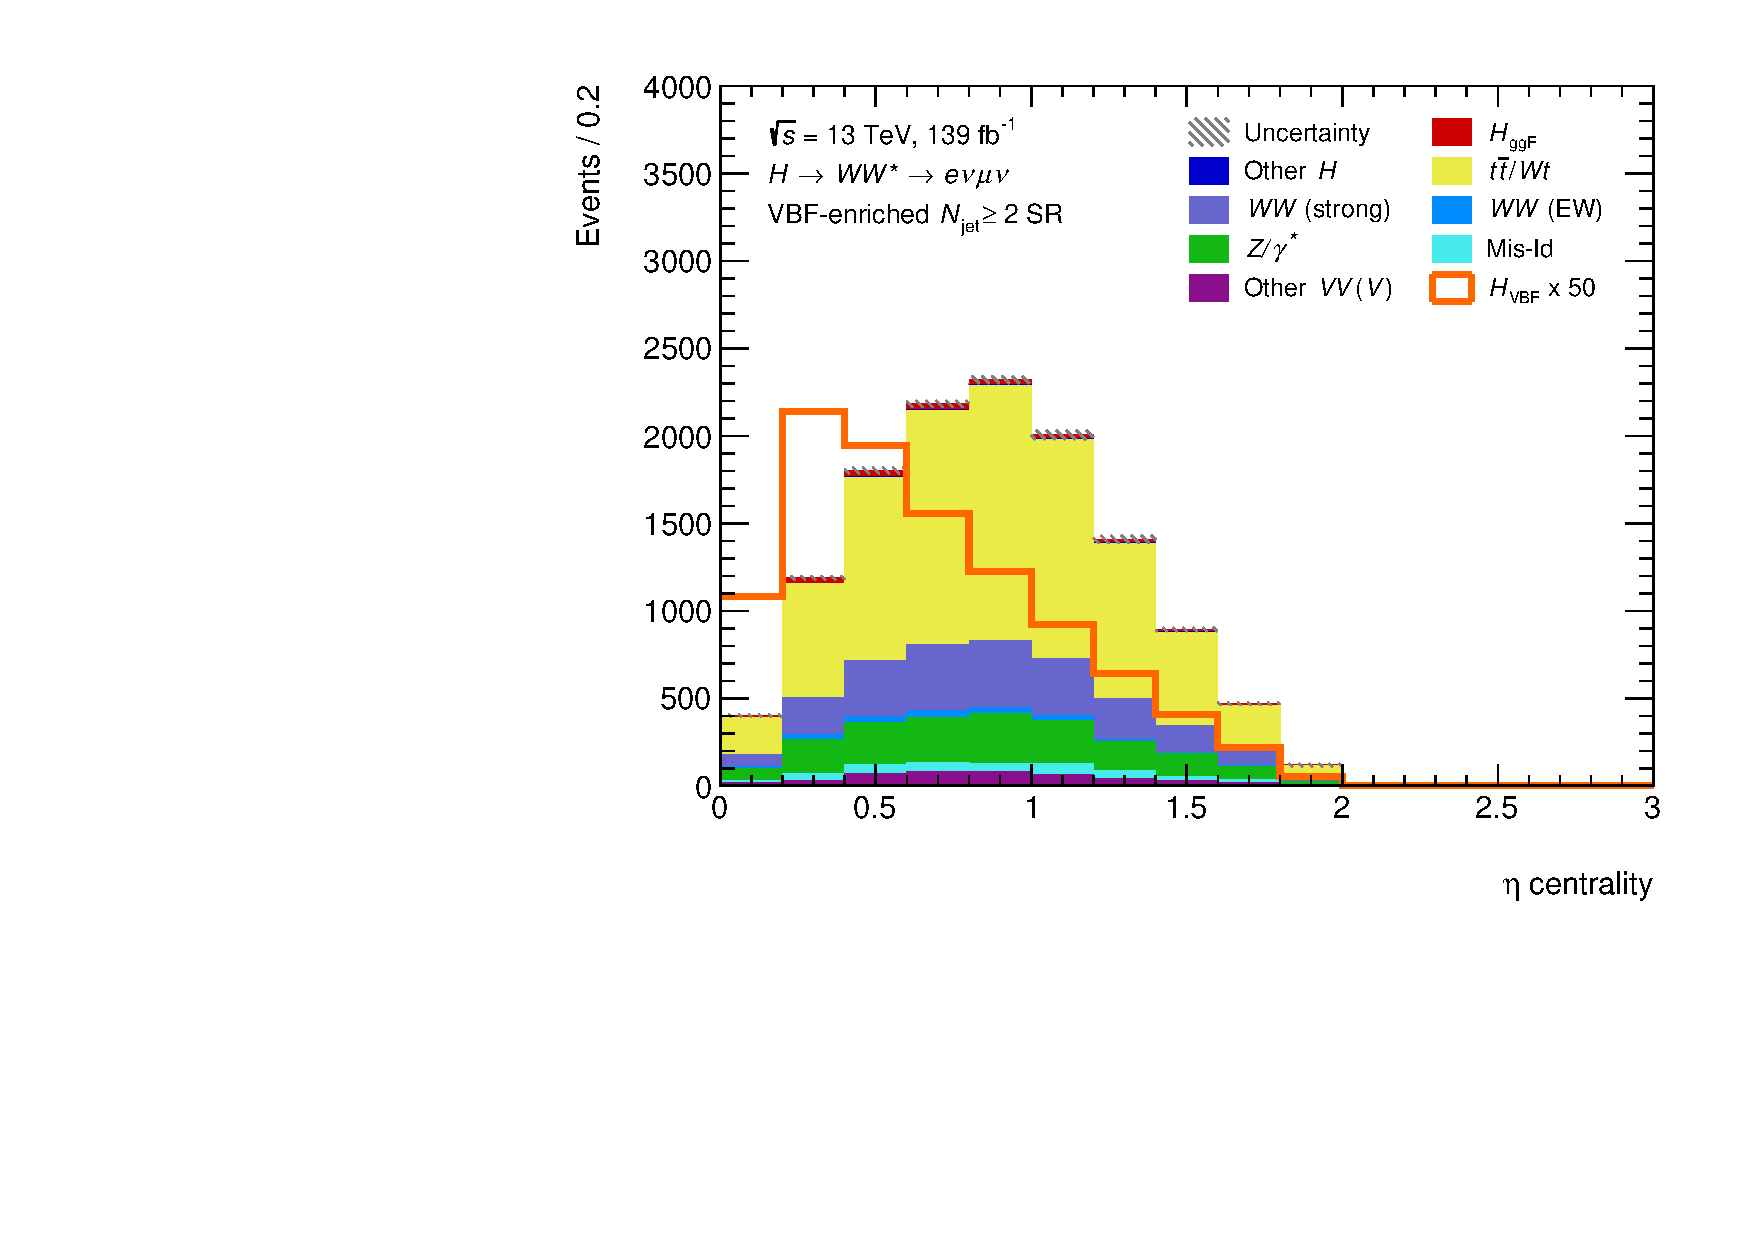
\includegraphics[width=0.32\textwidth]{figures/hww/dnn/blinded/run2-emme-CutVBF_SR-contOLV-lin.pdf} \hfill
        \label{fig:dnn-inputs-post-fit-3}
    } \\
    \subfloat[$\mlonejtwo$]{
        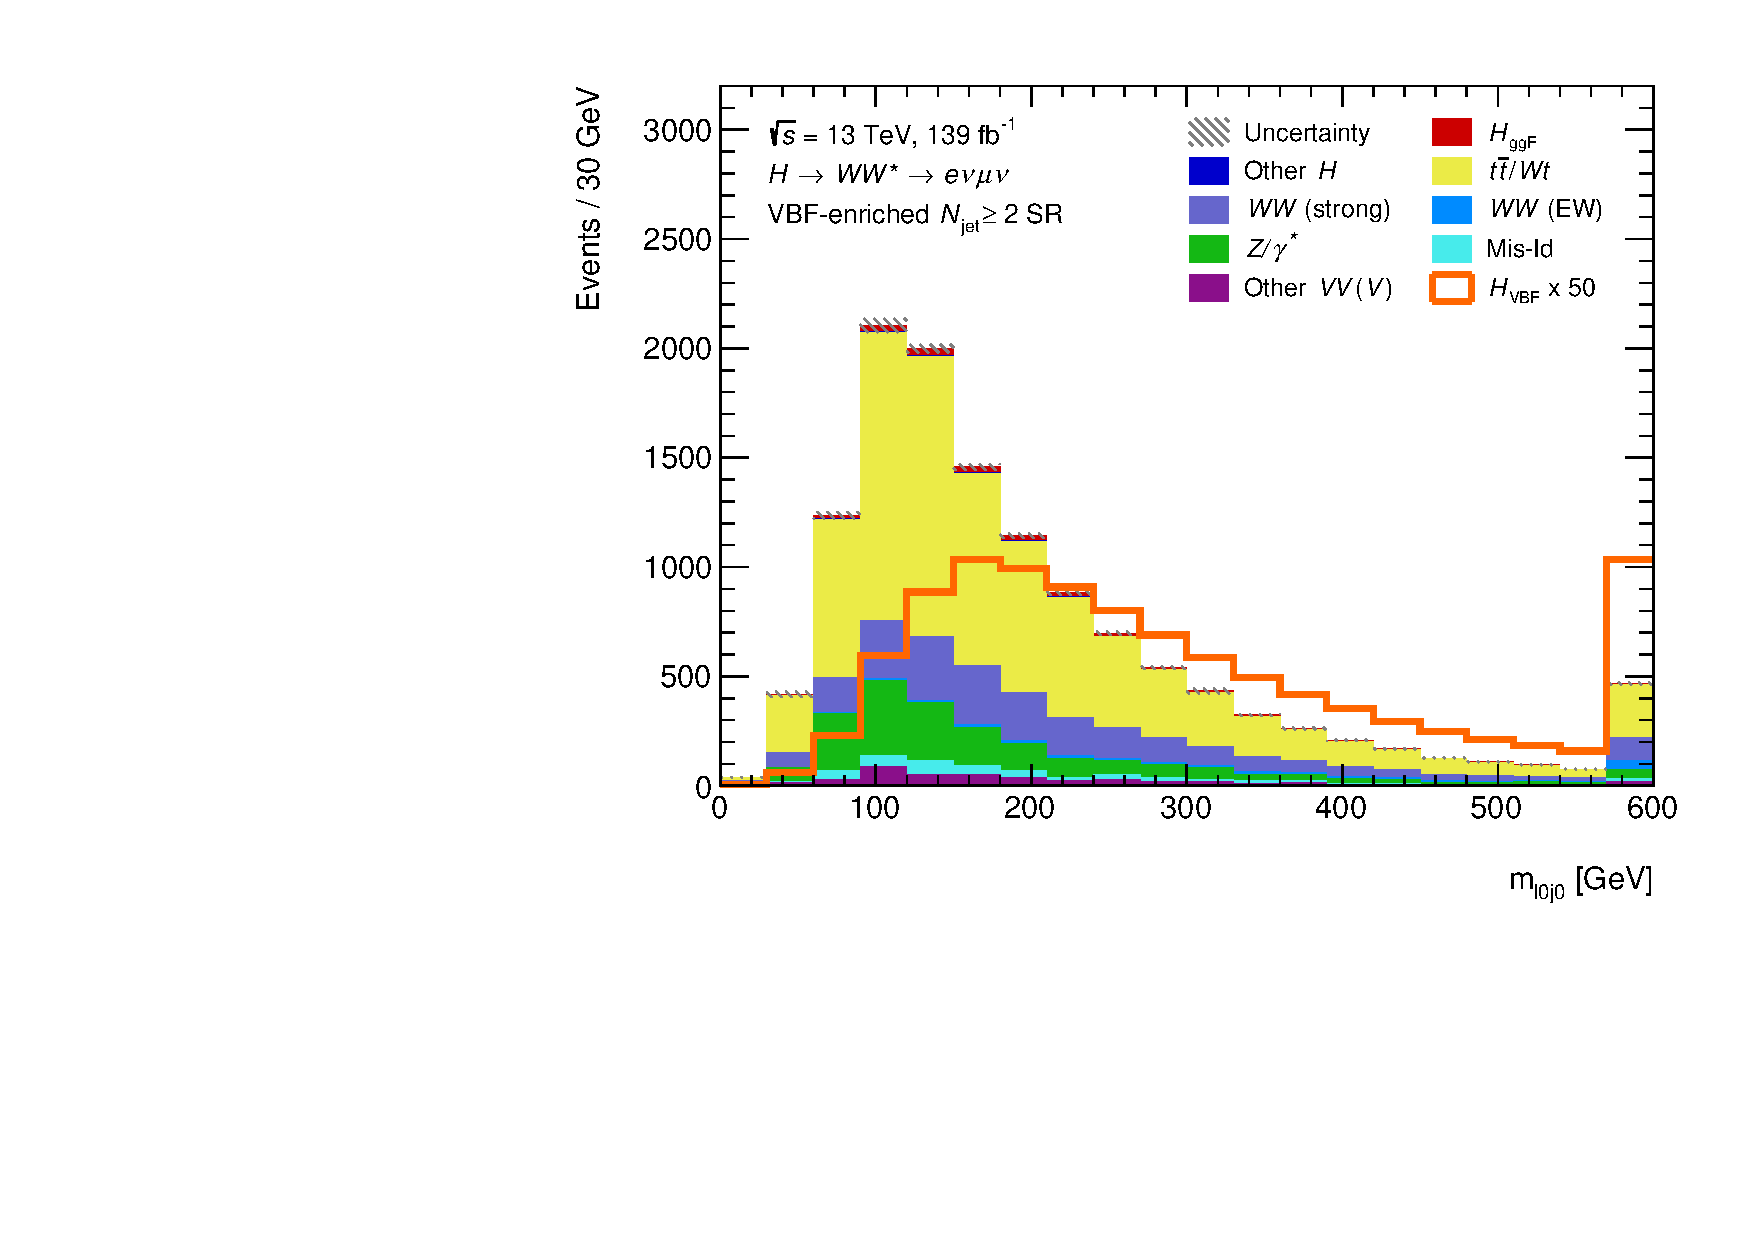
\includegraphics[width=0.32\textwidth]{figures/hww/dnn/blinded/run2-emme-CutVBF_SR-Ml0j0-lin.pdf} \hfill
        \label{fig:dnn-inputs-post-fit-4}
    } 
    \subfloat[$\mltwojone$]{
        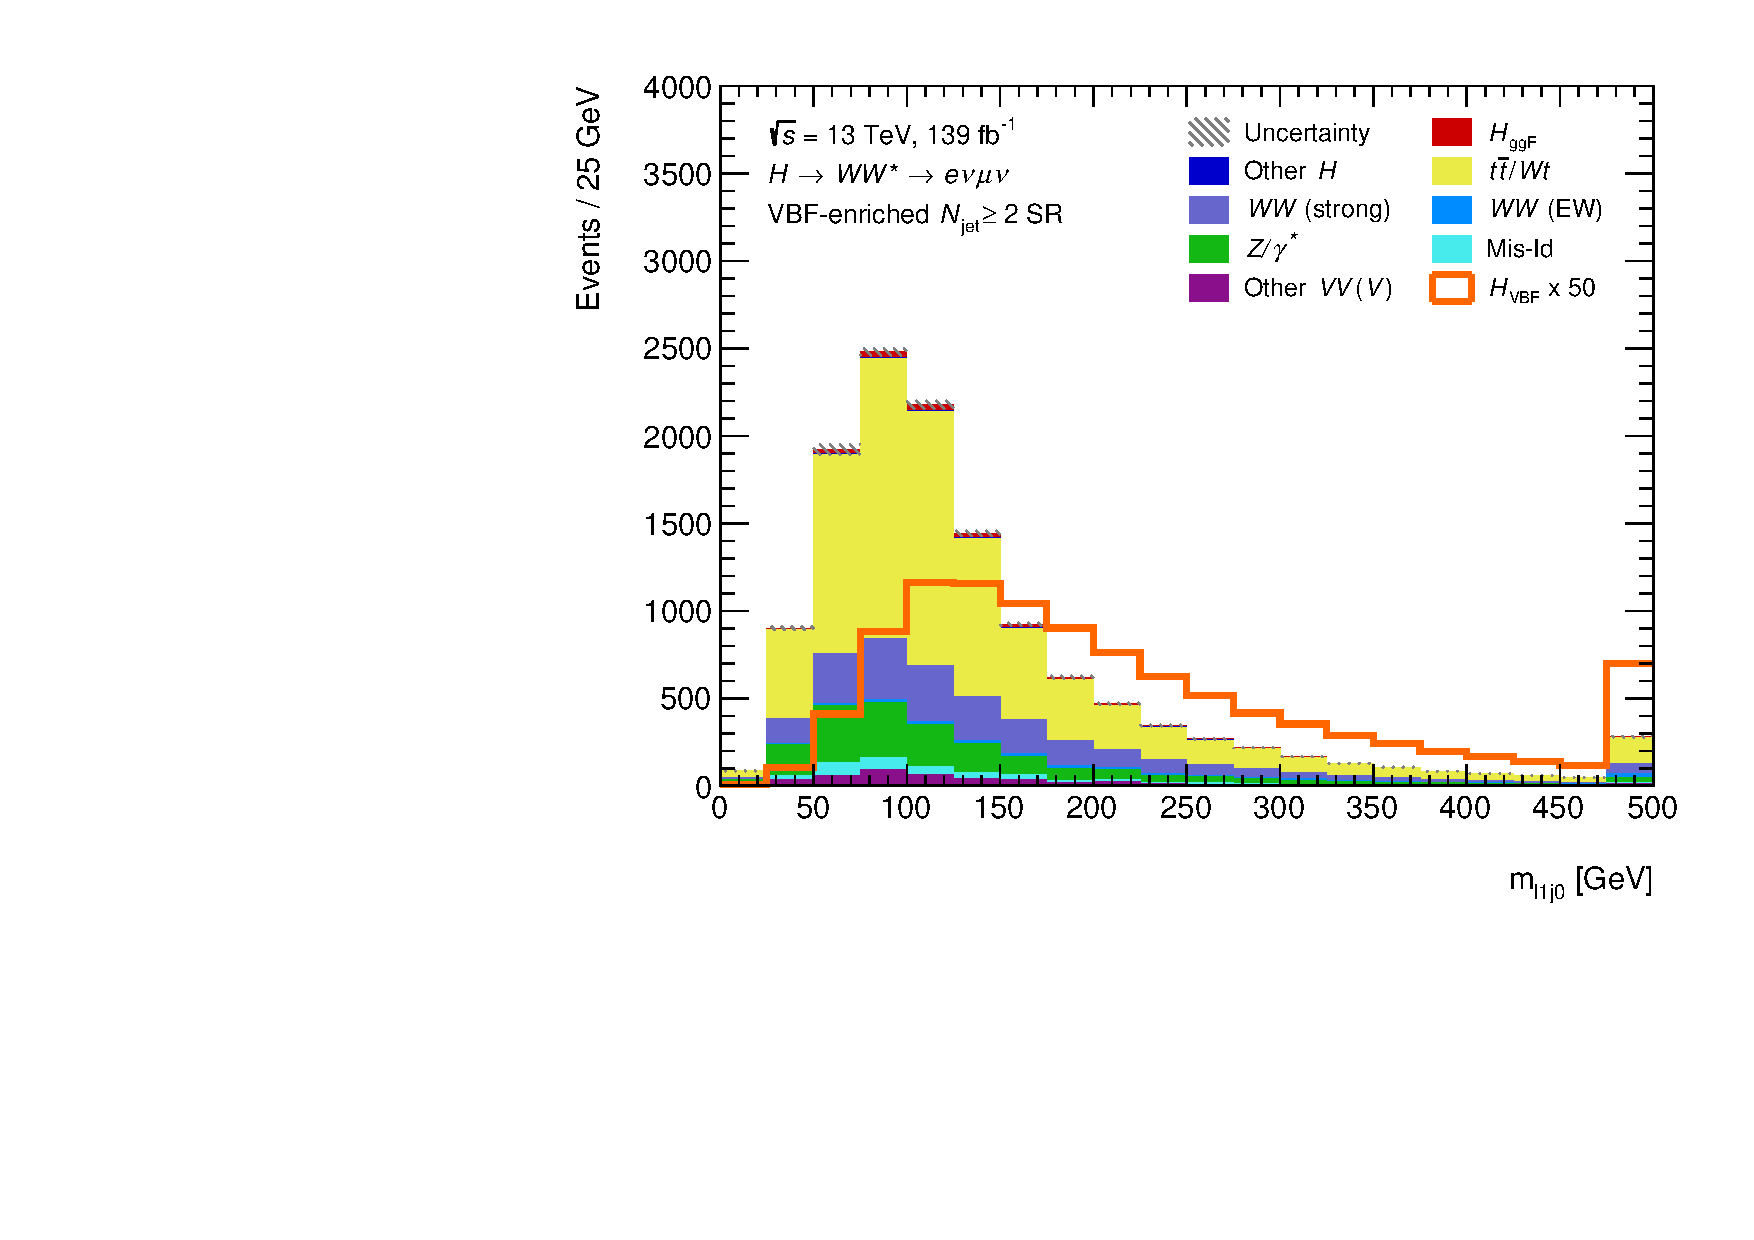
\includegraphics[width=0.32\textwidth]{figures/hww/dnn/blinded/run2-emme-CutVBF_SR-Ml1j0-lin.pdf} \hfill
        \label{fig:dnn-inputs-post-fit-5}
    } 
    \subfloat[$\mlonejtwo$]{
        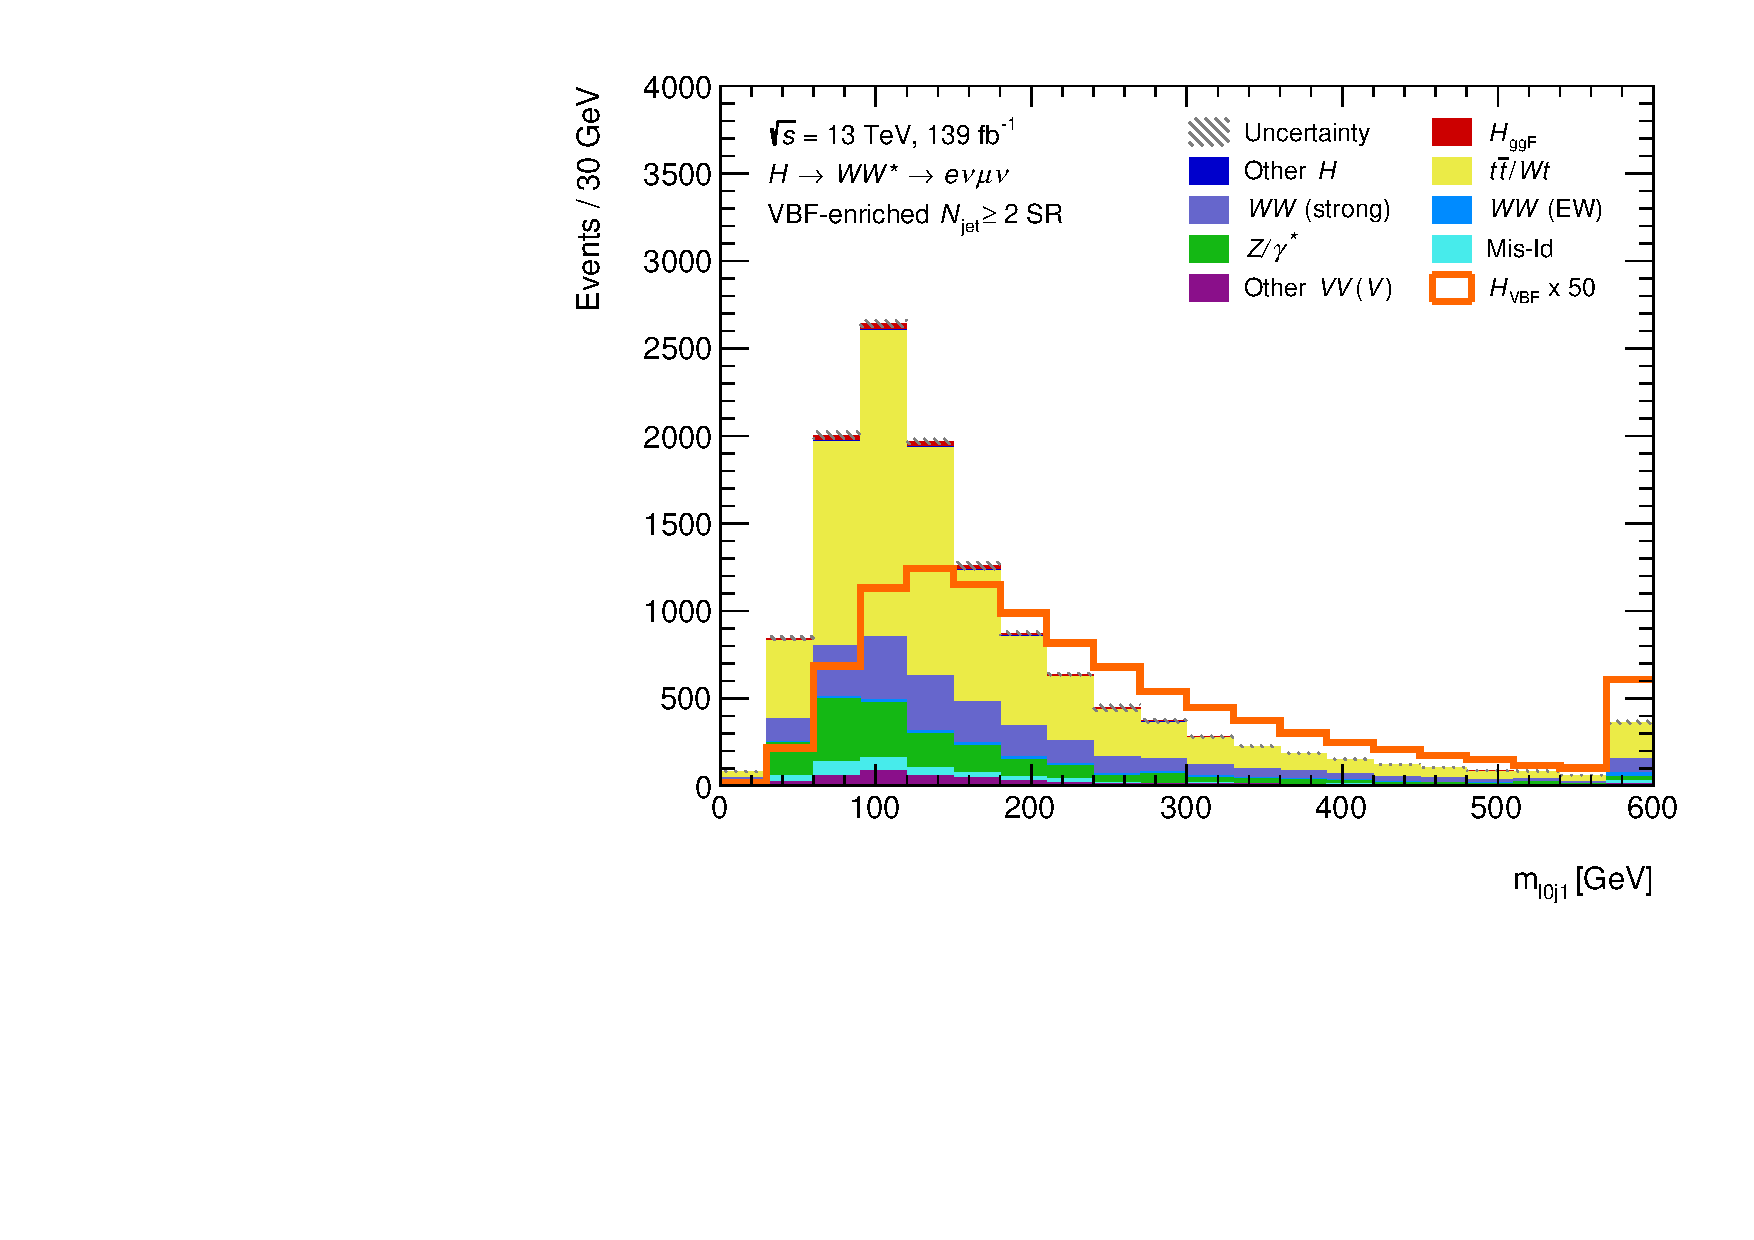
\includegraphics[width=0.32\textwidth]{figures/hww/dnn/blinded/run2-emme-CutVBF_SR-Ml0j1-lin.pdf} \hfill
        \label{fig:dnn-inputs-post-fit-6}
    } \\
    \subfloat[$\mltwojtwo$]{
        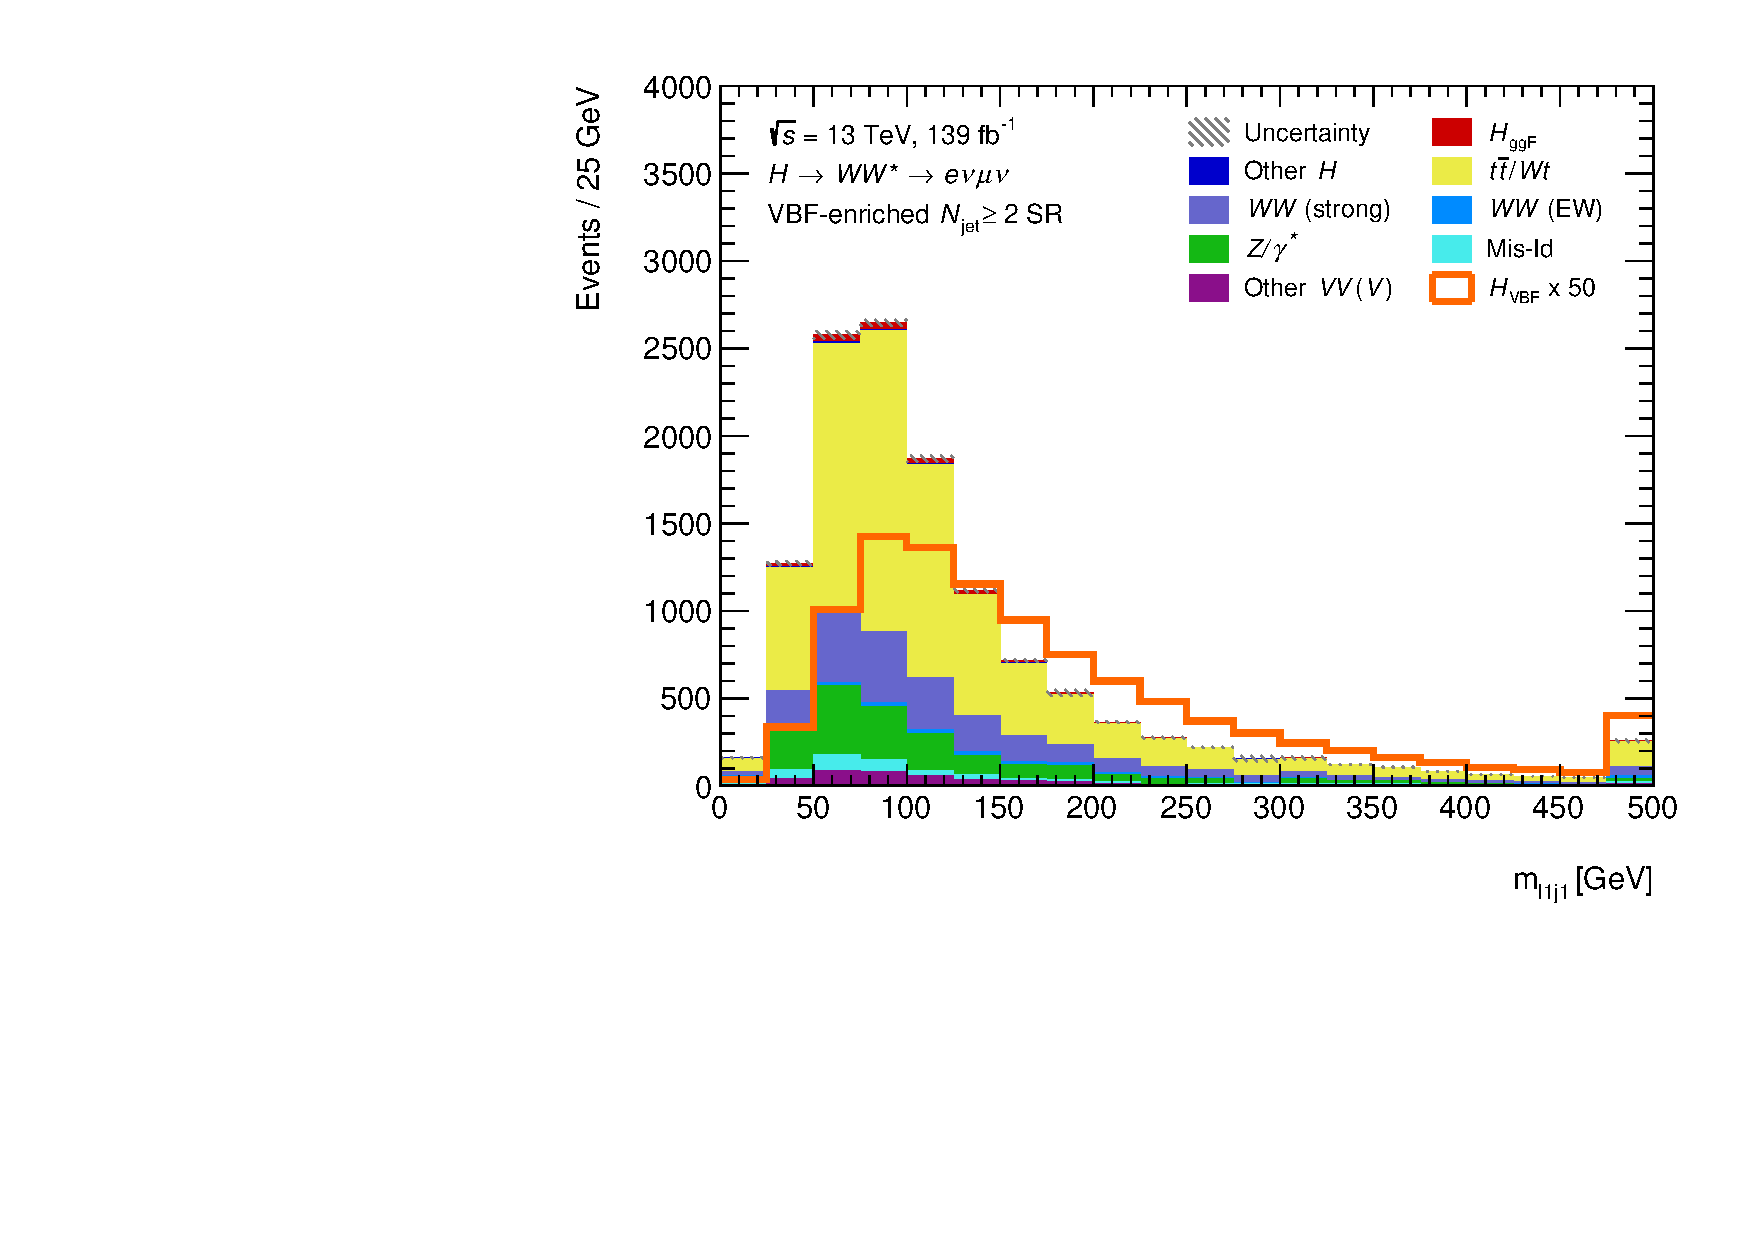
\includegraphics[width=0.32\textwidth]{figures/hww/dnn/blinded/run2-emme-CutVBF_SR-Ml1j1-lin.pdf} \hfill
        \label{fig:dnn-inputs-post-fit-7}
    } 
    \subfloat[$\pTjone$]{
        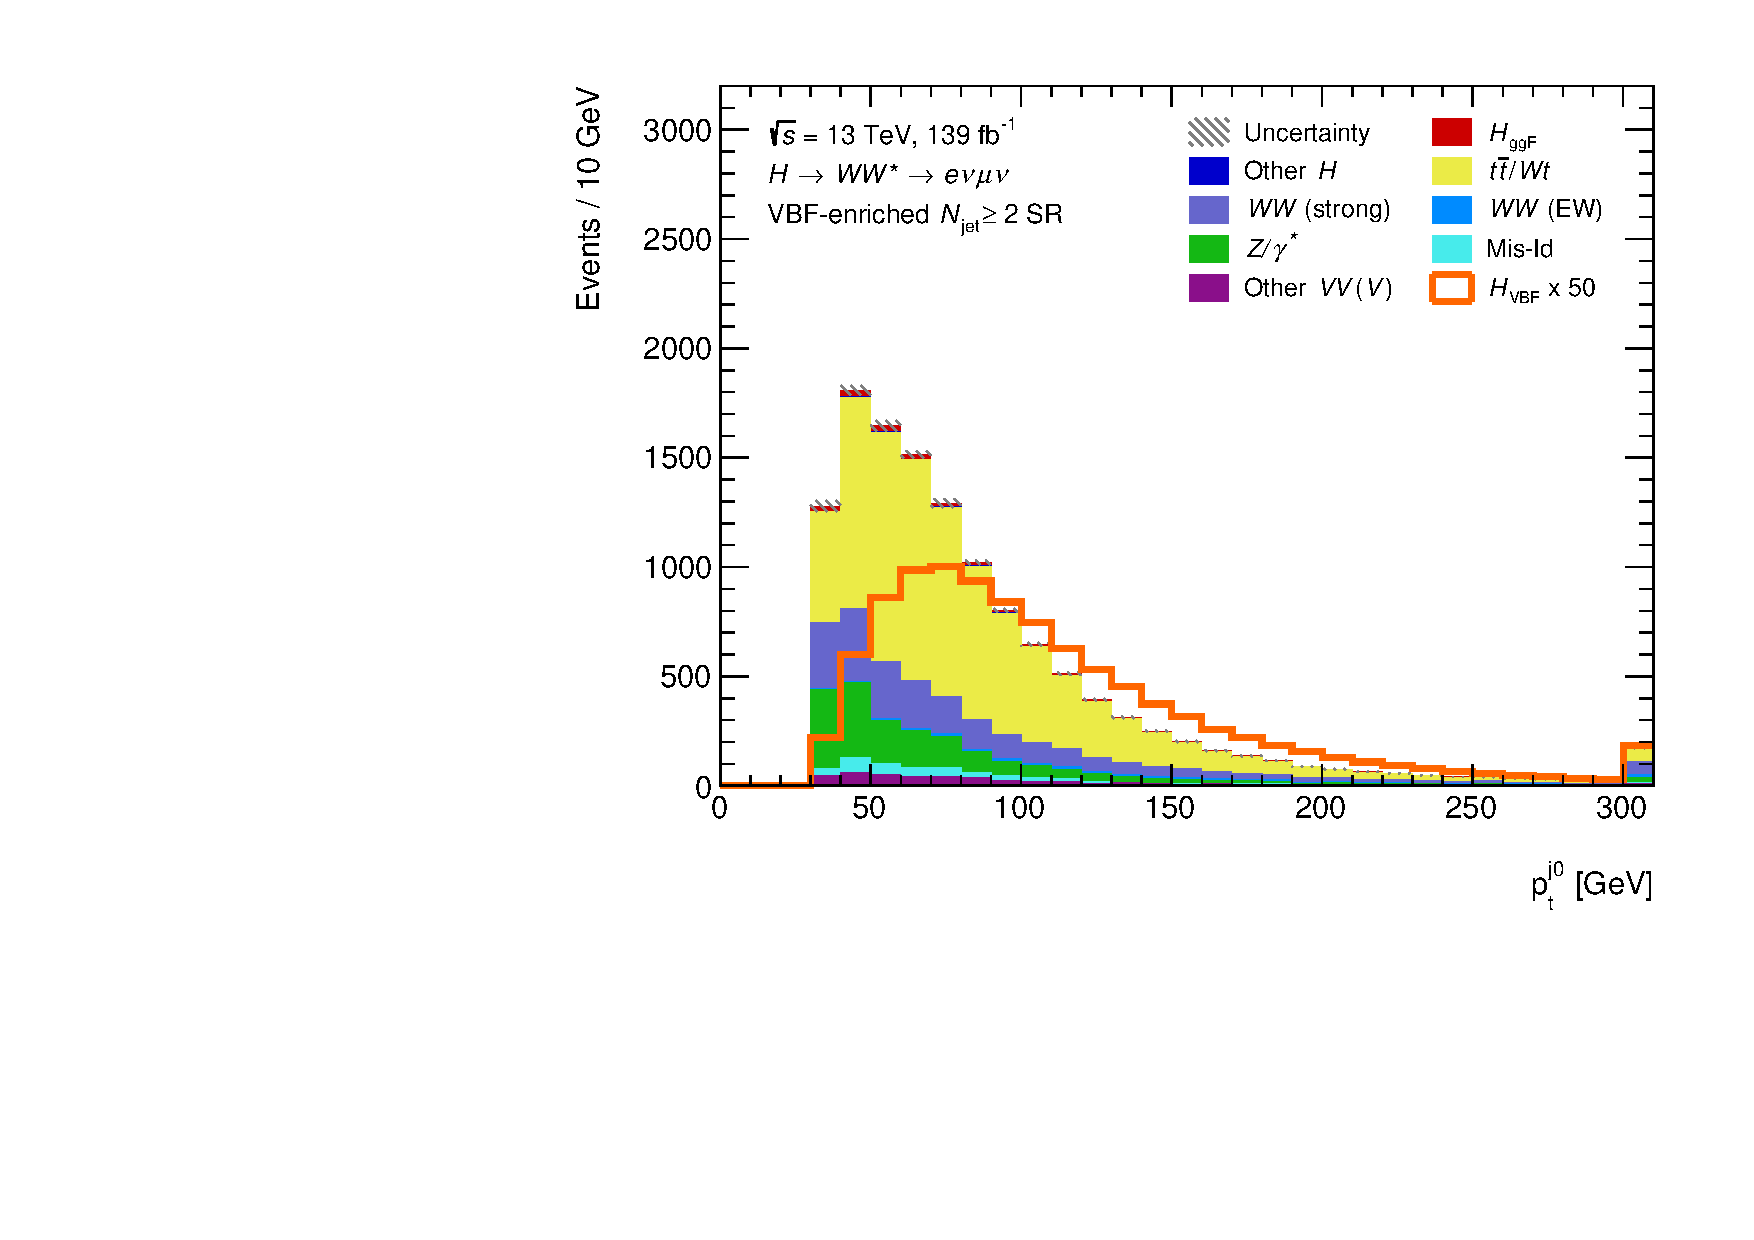
\includegraphics[width=0.32\textwidth]{figures/hww/dnn/blinded/run2-emme-CutVBF_SR-leadJetPt-lin.pdf} \hfill
        \label{fig:dnn-inputs-post-fit-8}
    } 
    \subfloat[$\pTjtwo$]{
        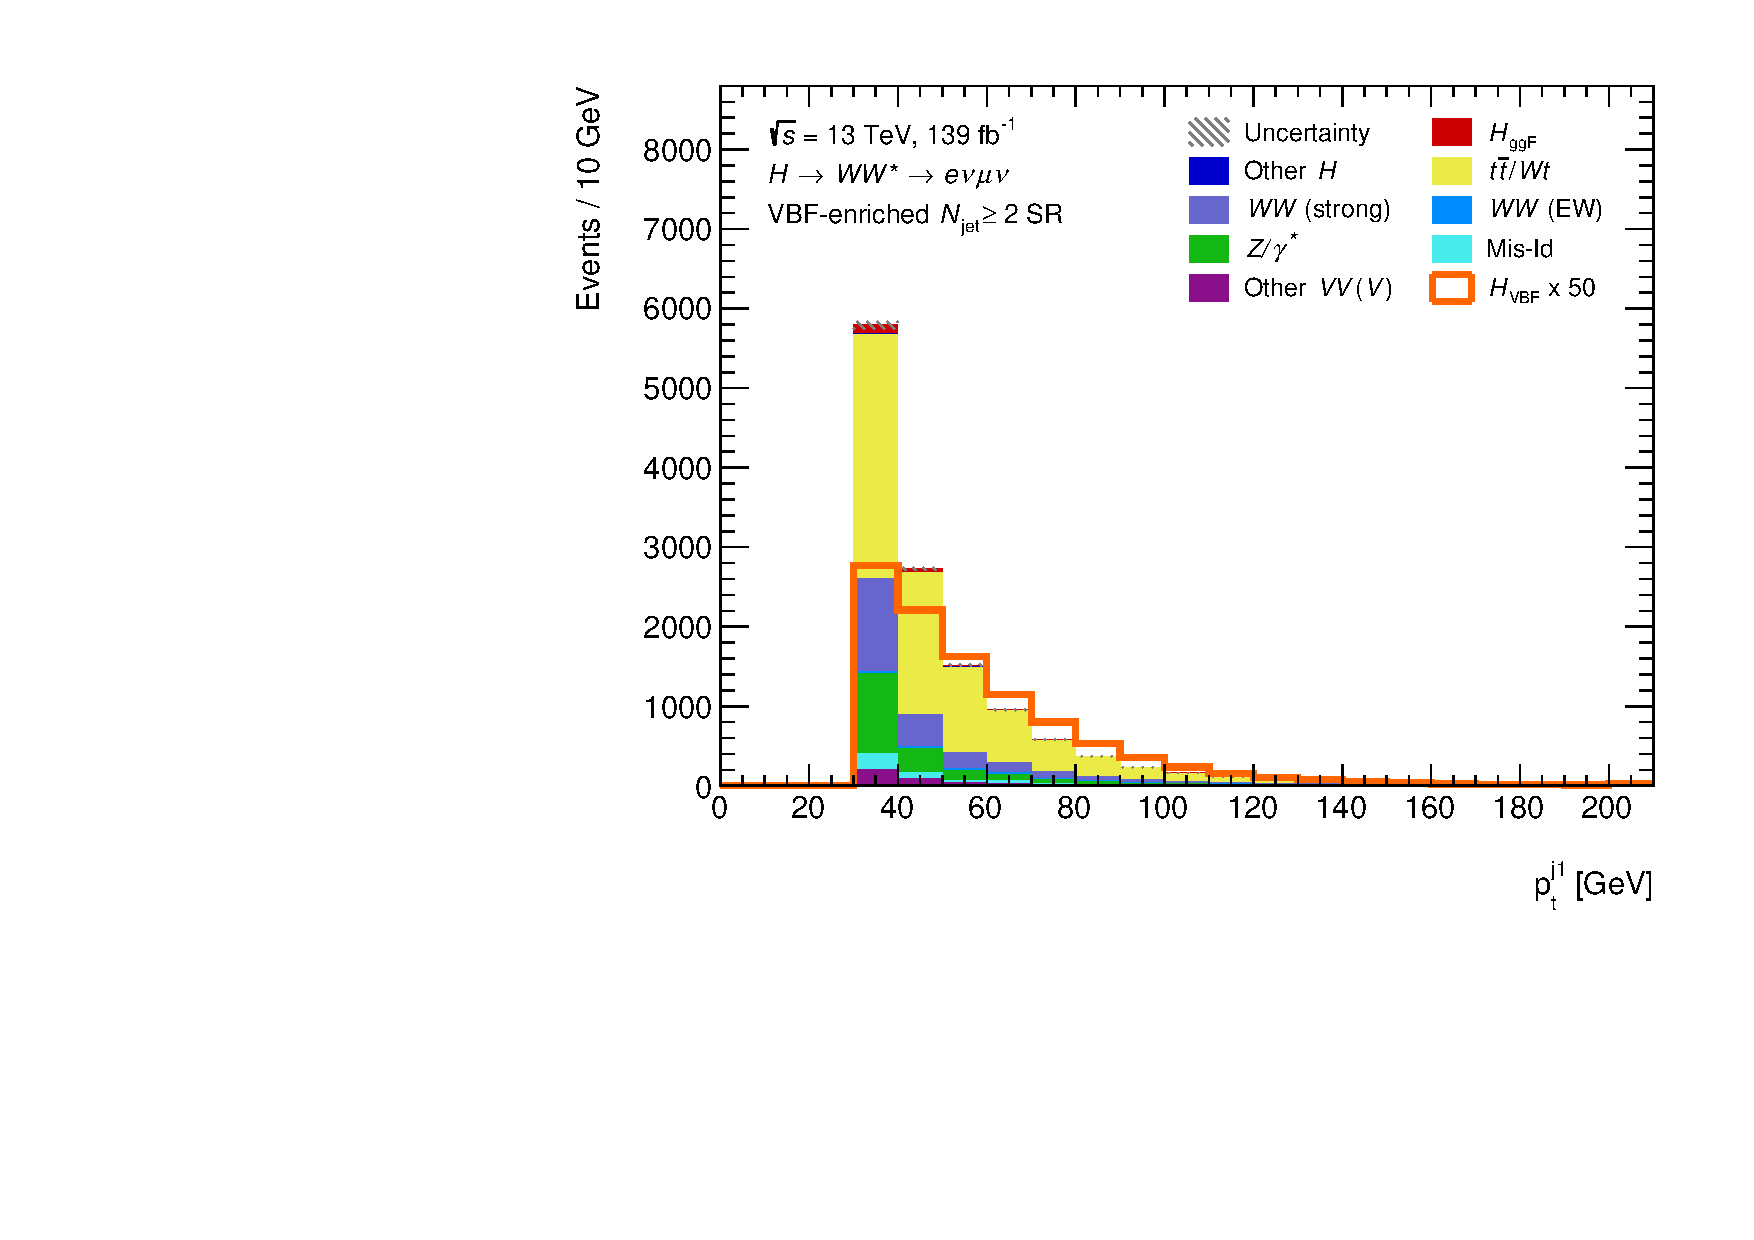
\includegraphics[width=0.32\textwidth]{figures/hww/dnn/blinded/run2-emme-CutVBF_SR-subleadJetPt-lin.pdf} \hfill
        \label{fig:dnn-inputs-post-fit-9}
    } \\
    \subfloat[$\pTjthree$]{
        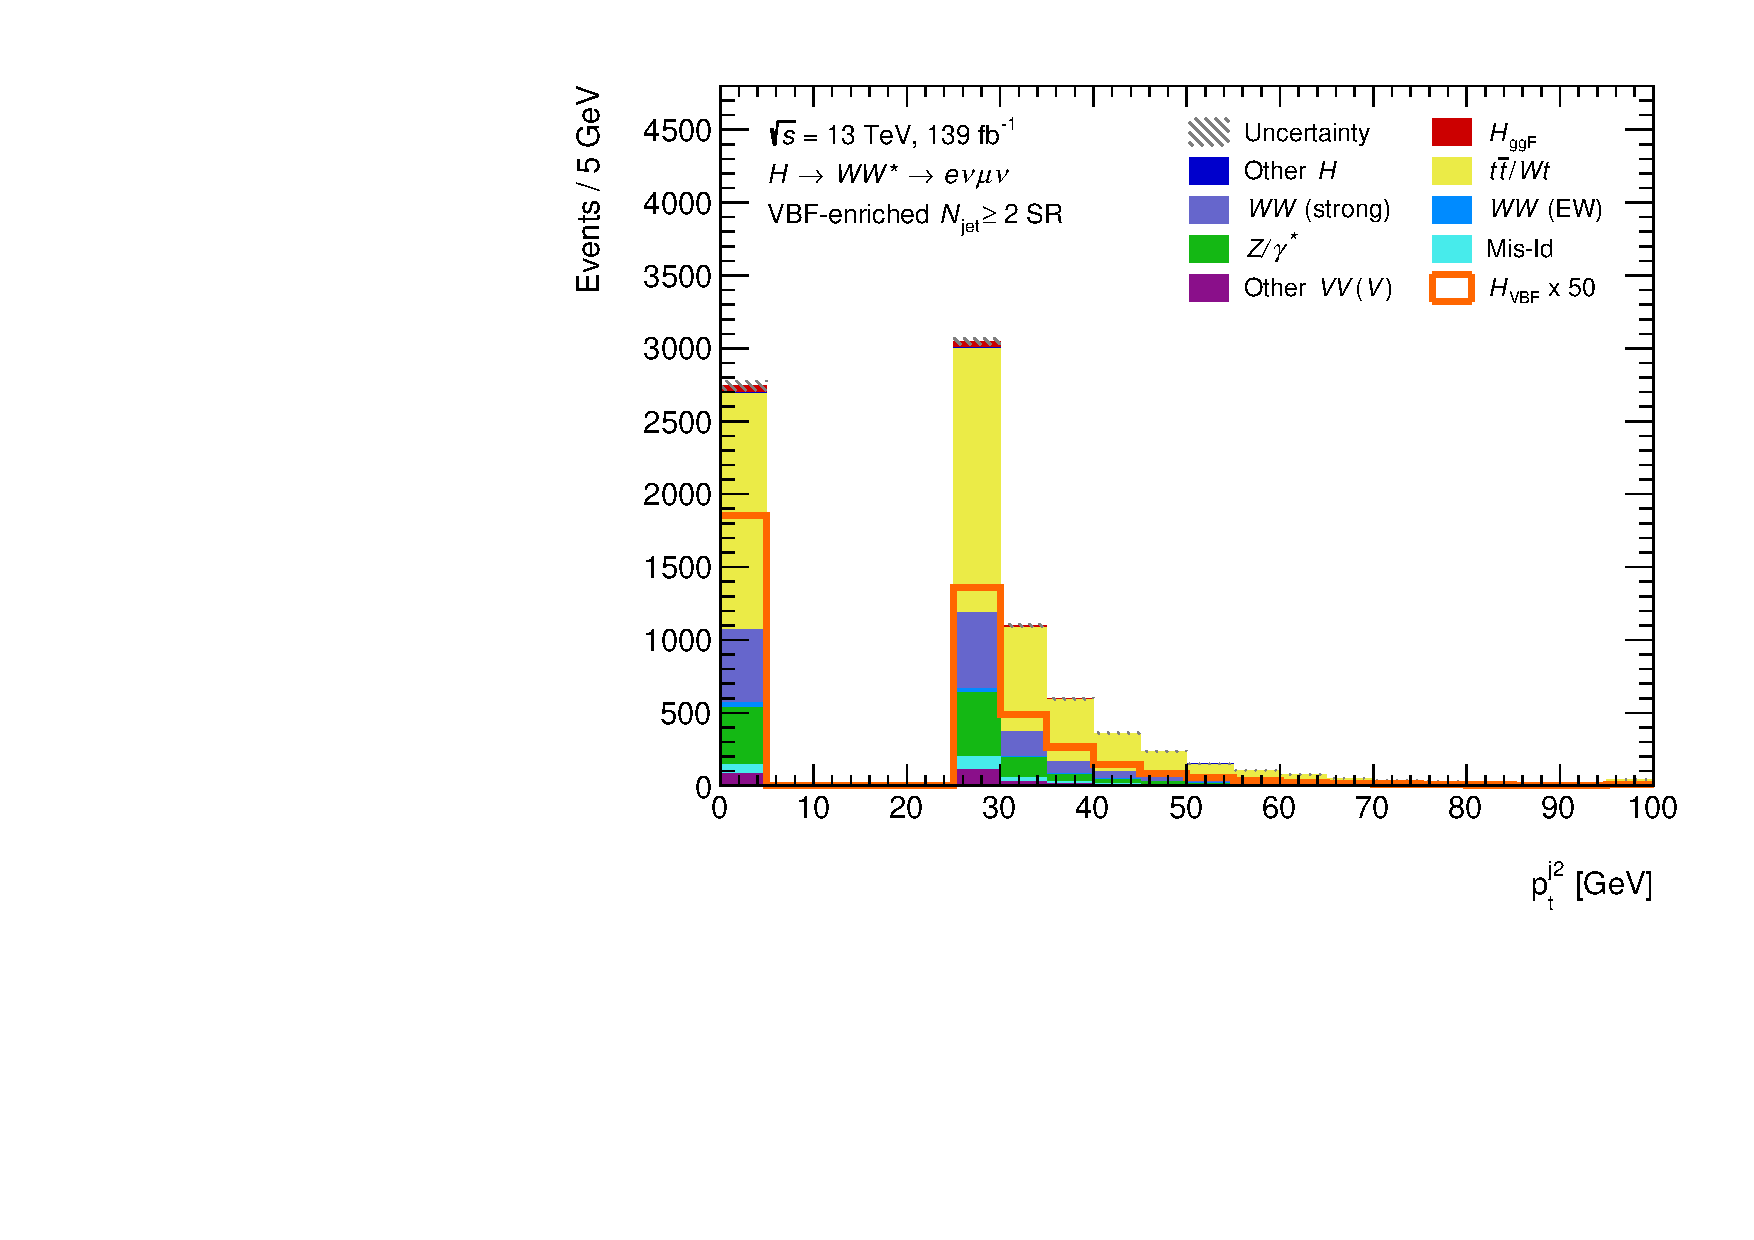
\includegraphics[width=0.32\textwidth]{figures/hww/dnn/blinded/run2-emme-CutVBF_SR-thirdJetPt-lin.pdf} \hfill
        \label{fig:dnn-inputs-post-fit-10}
    } 
    {\caption{Distributions of $\dphill$, $\mll$, $\lepetacent$, \pTjone, \pTjtwo, \pTjthree in the VBF signal region.
        Each row corresponds to one variable with different selections made on the DNN output.
        \label{fig:dnn-inputs-post-fit1} }}
\end{figure}


% \begin{figure}[h]
%     \centering
%     {\caption{Distributions of $\mlonejone$, $\mltwojone$, $\mlonejtwo$, and $\mltwojtwo$ in the VBF signal region.
%             Each row shows one variable with different cuts on the DNN output distribution being applied in different columns.
%             \label{app:fig:dnn-inputs-vbf-top2} }}
% \end{figure}


\begin{figure}[h]
    \centering
    \subfloat[$\dphill$]{
        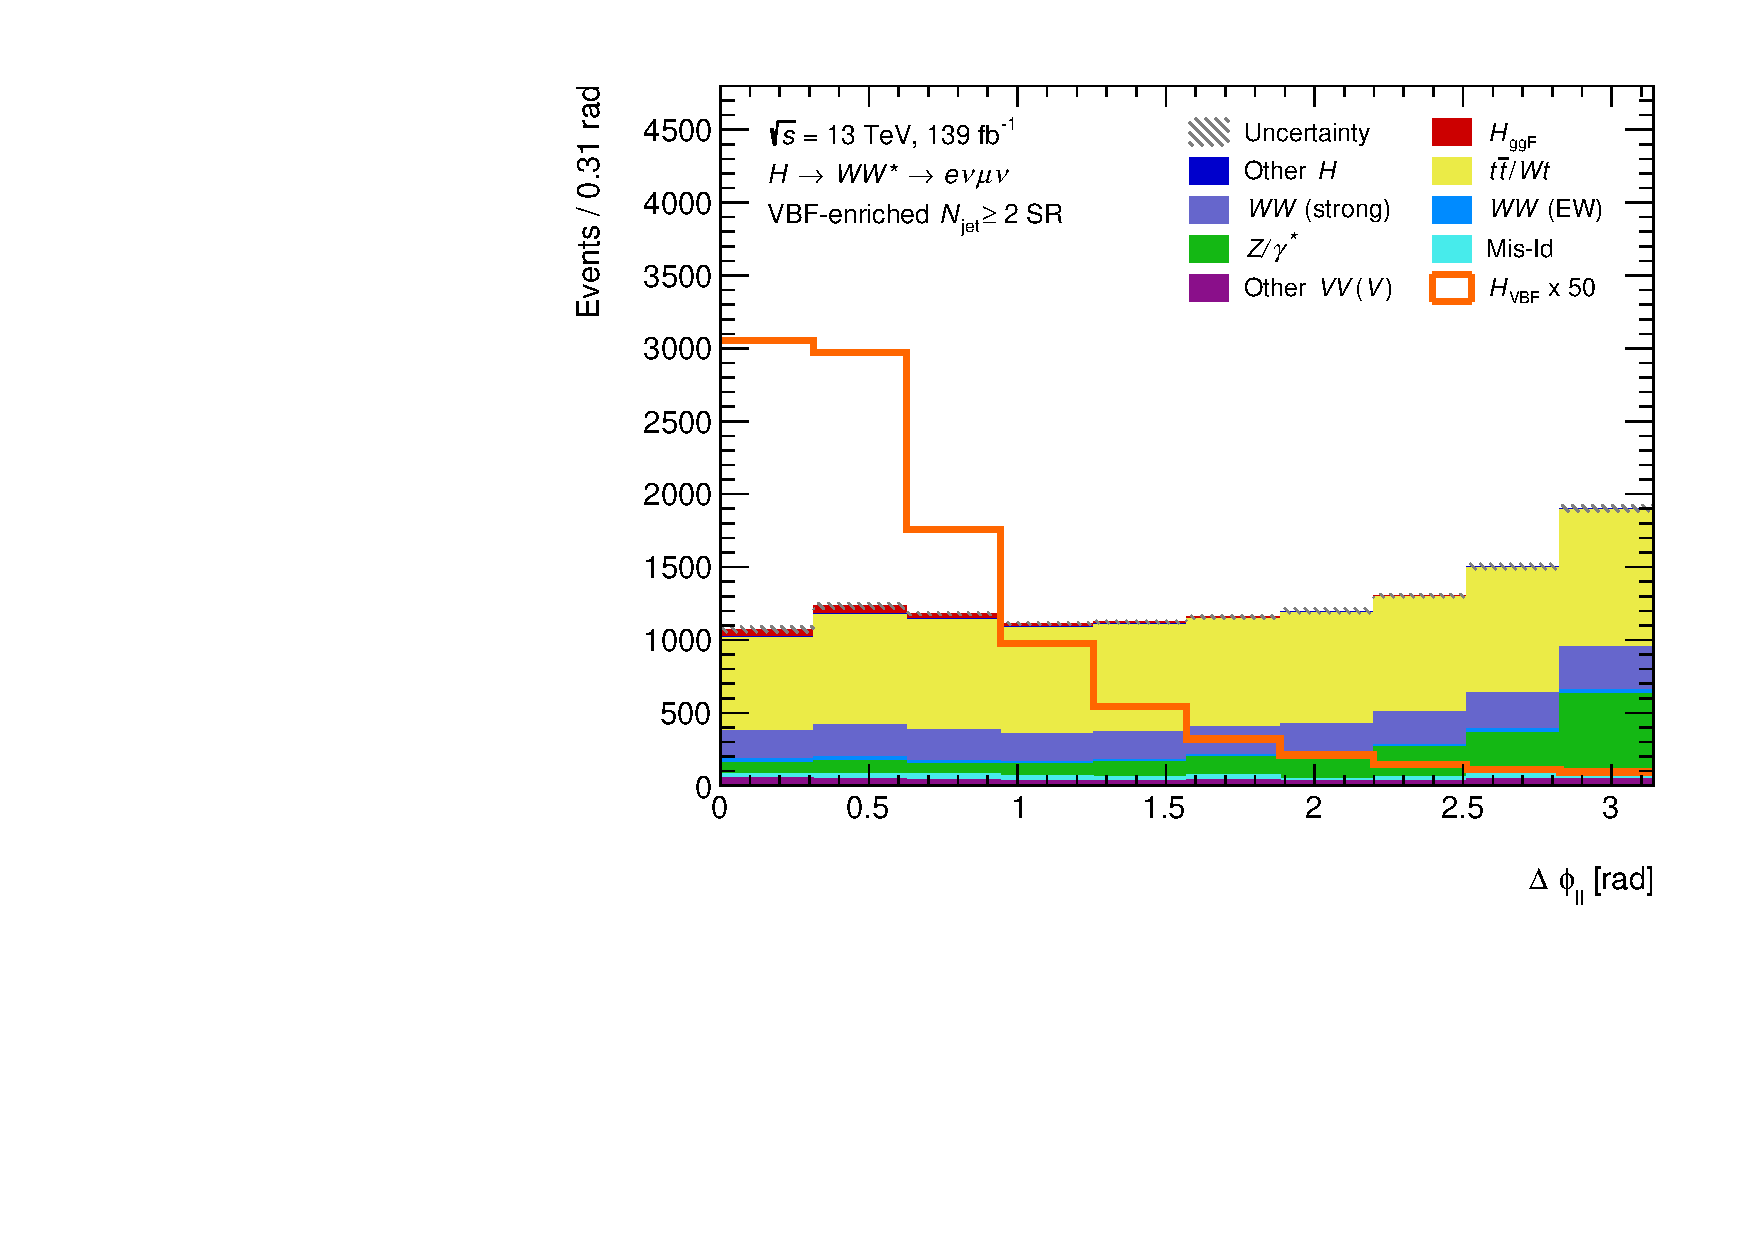
\includegraphics[width=0.32\textwidth]{figures/hww/dnn/blinded/run2-emme-CutVBF_SR-DPhill-lin.pdf} \hfill
        \label{fig:dnn-inputs-post-fit2-1}
    } 
    \subfloat[$\mll$]{
        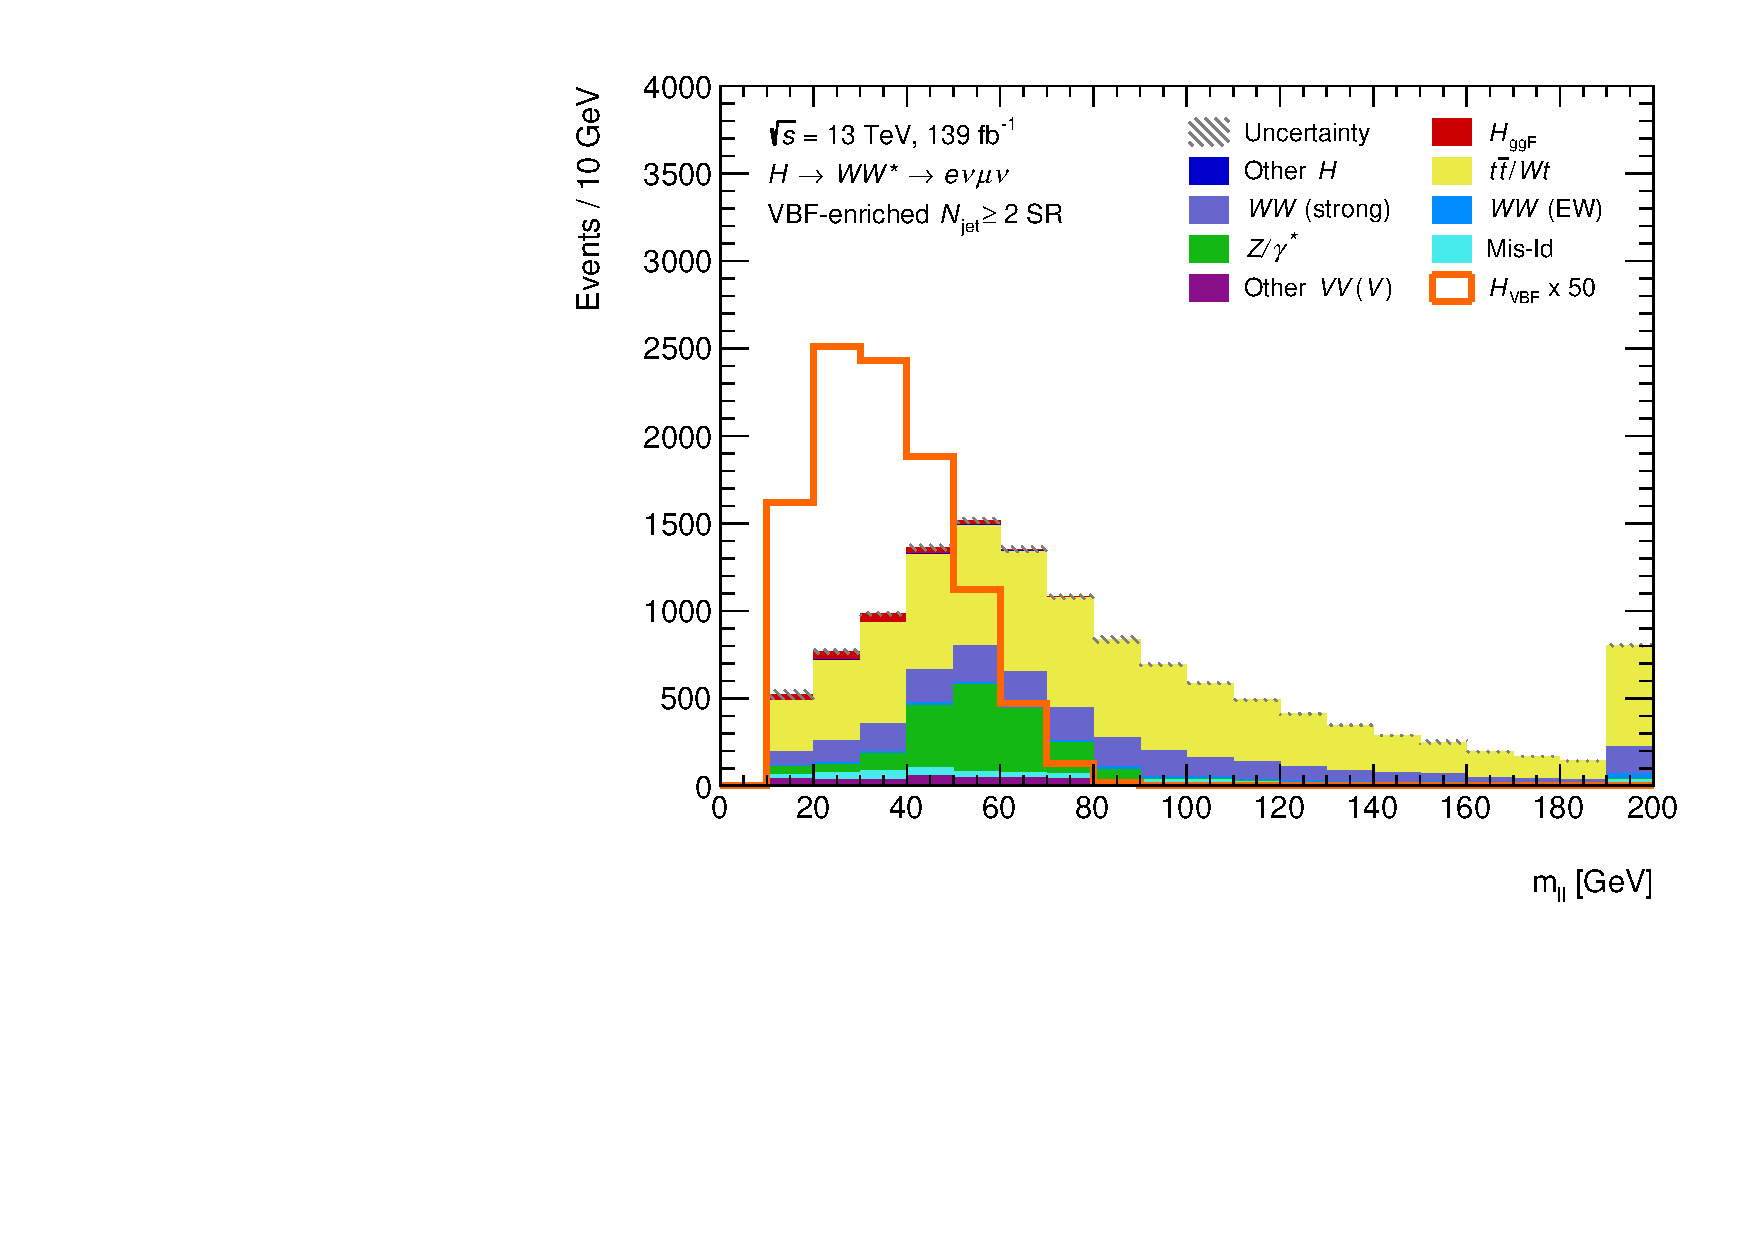
\includegraphics[width=0.32\textwidth]{figures/hww/dnn/blinded/run2-emme-CutVBF_SR-Mll-lin.pdf}
        \label{fig:dnn-inputs-post-fit2-2}
    } 
    \subfloat[$\mT$]{
        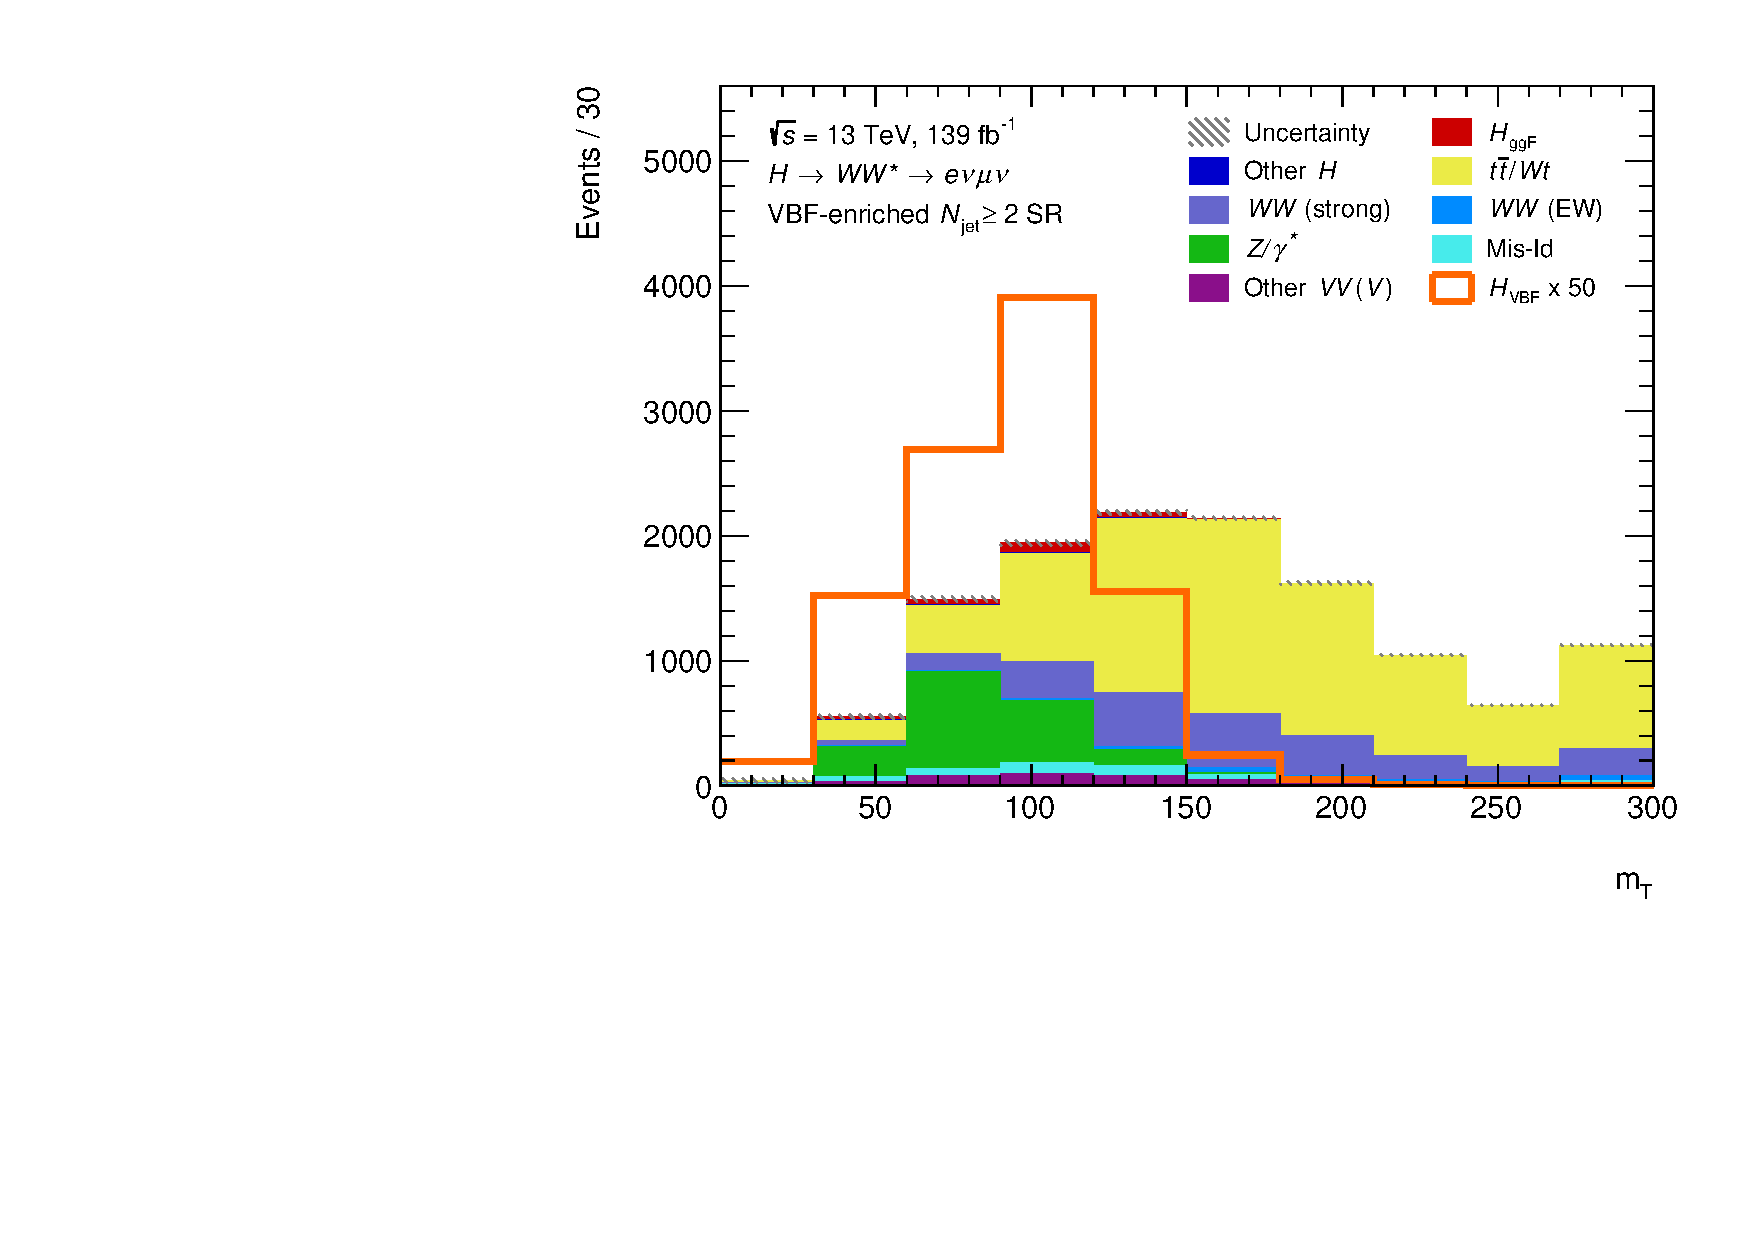
\includegraphics[width=0.32\textwidth]{figures/hww/dnn/blinded/run2-emme-CutVBF_SR-MT-lin.pdf} \hfill
        \label{fig:dnn-inputs-post-fit2-3}
    } \\
    \subfloat[$\pttot$]{
        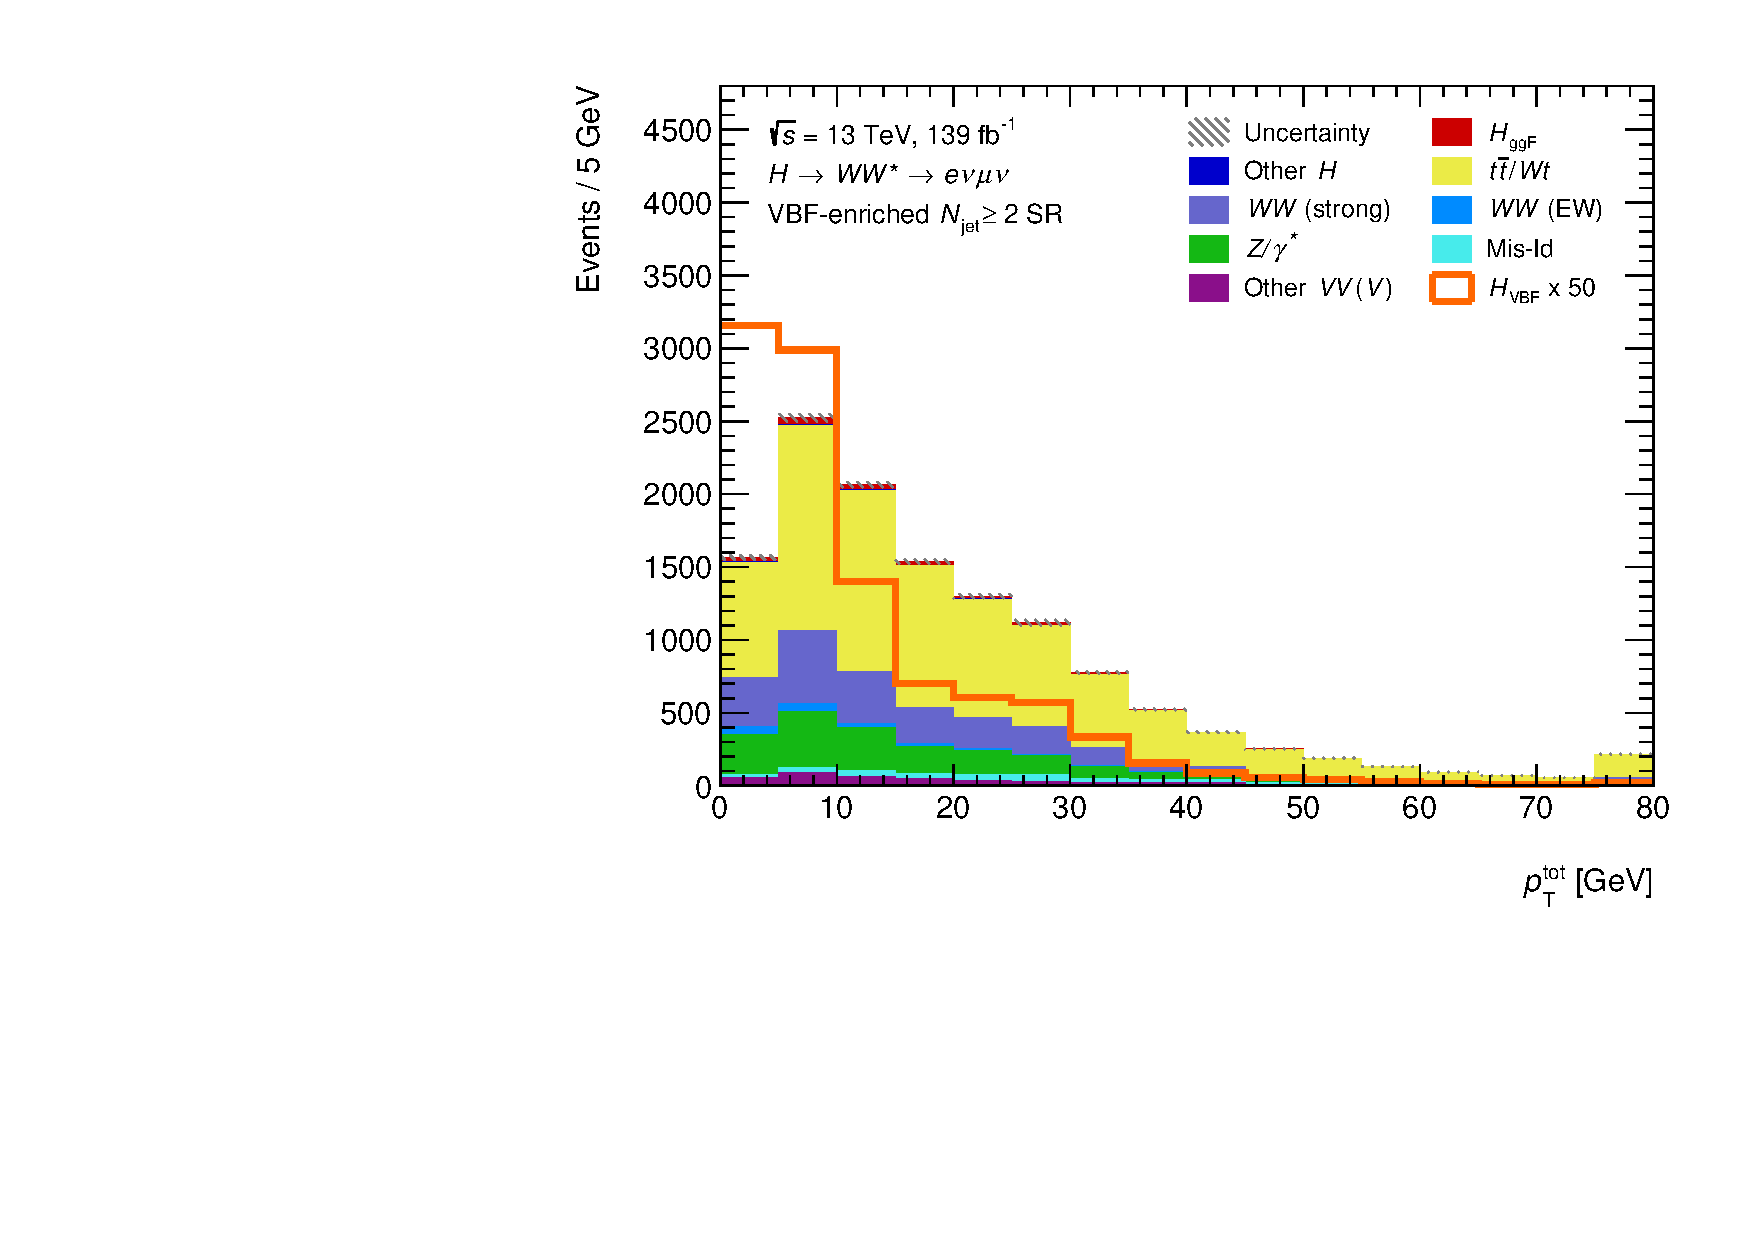
\includegraphics[width=0.32\textwidth]{figures/hww/dnn/blinded/run2-emme-CutVBF_SR-PtTot-lin.pdf} \hfill
        \label{fig:dnn-inputs-post-fit2-4}
    } 
    \subfloat[$\METSig$]{
        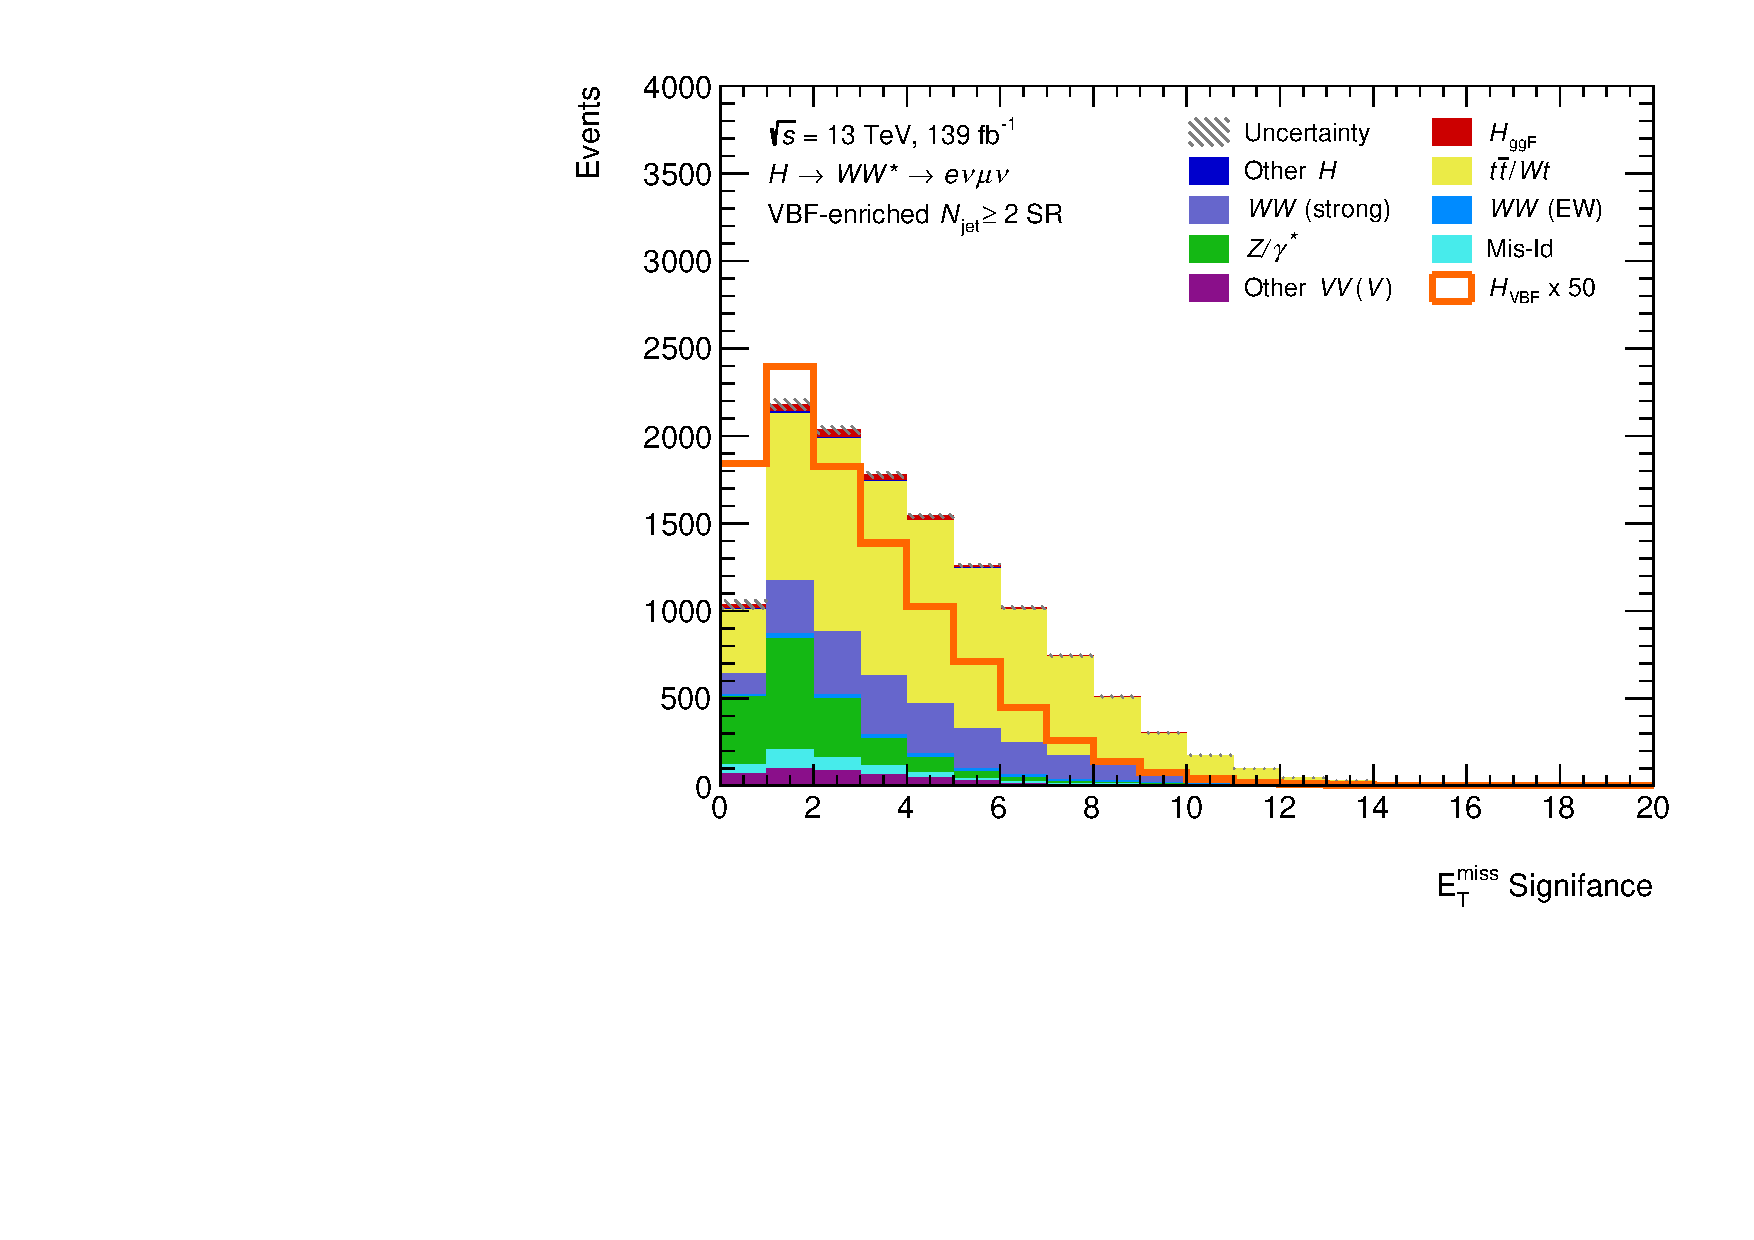
\includegraphics[width=0.32\textwidth]{figures/hww/dnn/blinded/run2-emme-CutVBF_SR-METSig_broad-lin.pdf} \hfill
        \label{fig:dnn-inputs-post-fit2-5}
    } 
    {\caption{Distributions of $\dphill$, $\mll$, $\mT$ in the VBF signal region.
        Each row corresponds to one variable with different selections made on the DNN output.
        \label{fig:dnn-inputs-post-fit2} }}
\end{figure}
}


\newcommand{\dnnfigures}{
\begin{figure}[h]
    \centering
    \subfloat[$\mjj$]{
        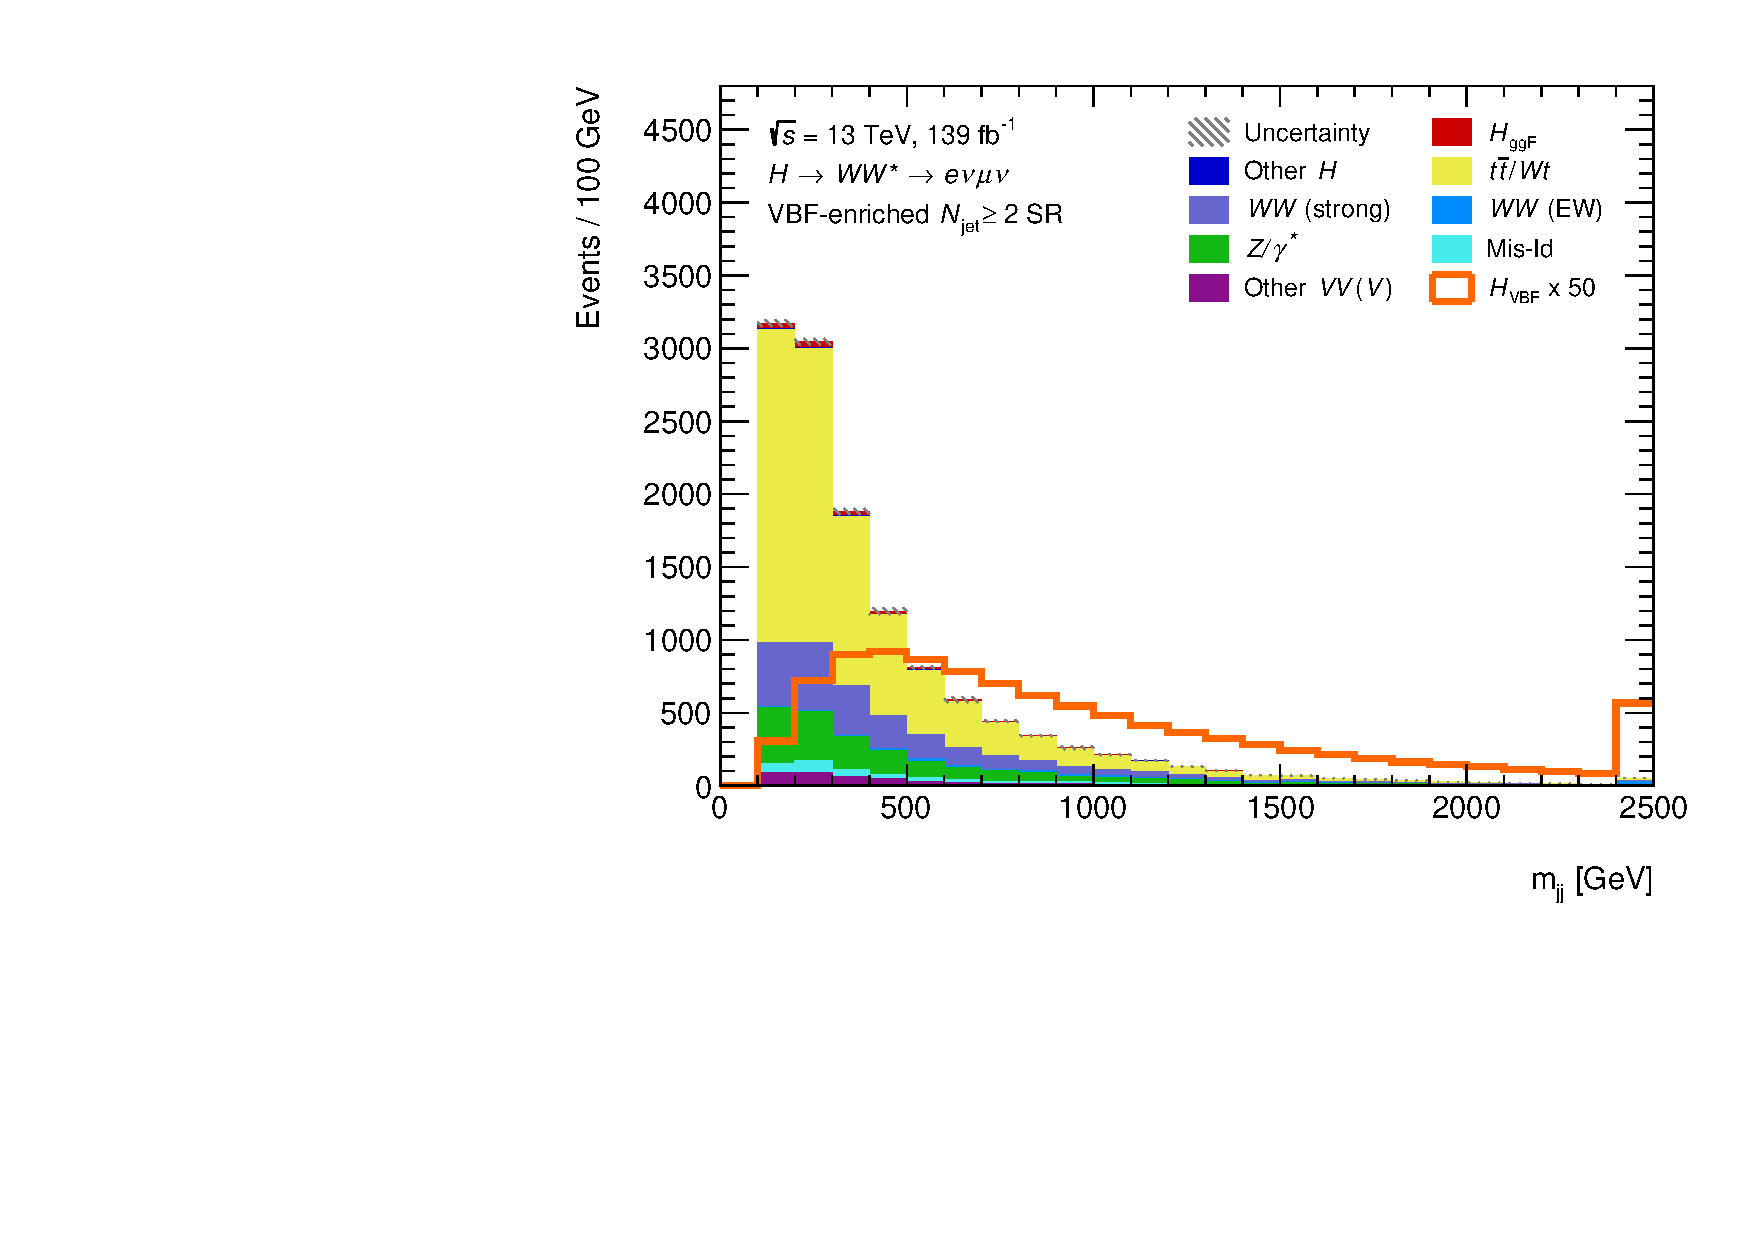
\includegraphics[width=0.32\textwidth]{figures/hww/dnn/blinded/run2-emme-CutVBF_SR-Mjj-lin.pdf} \hfill
        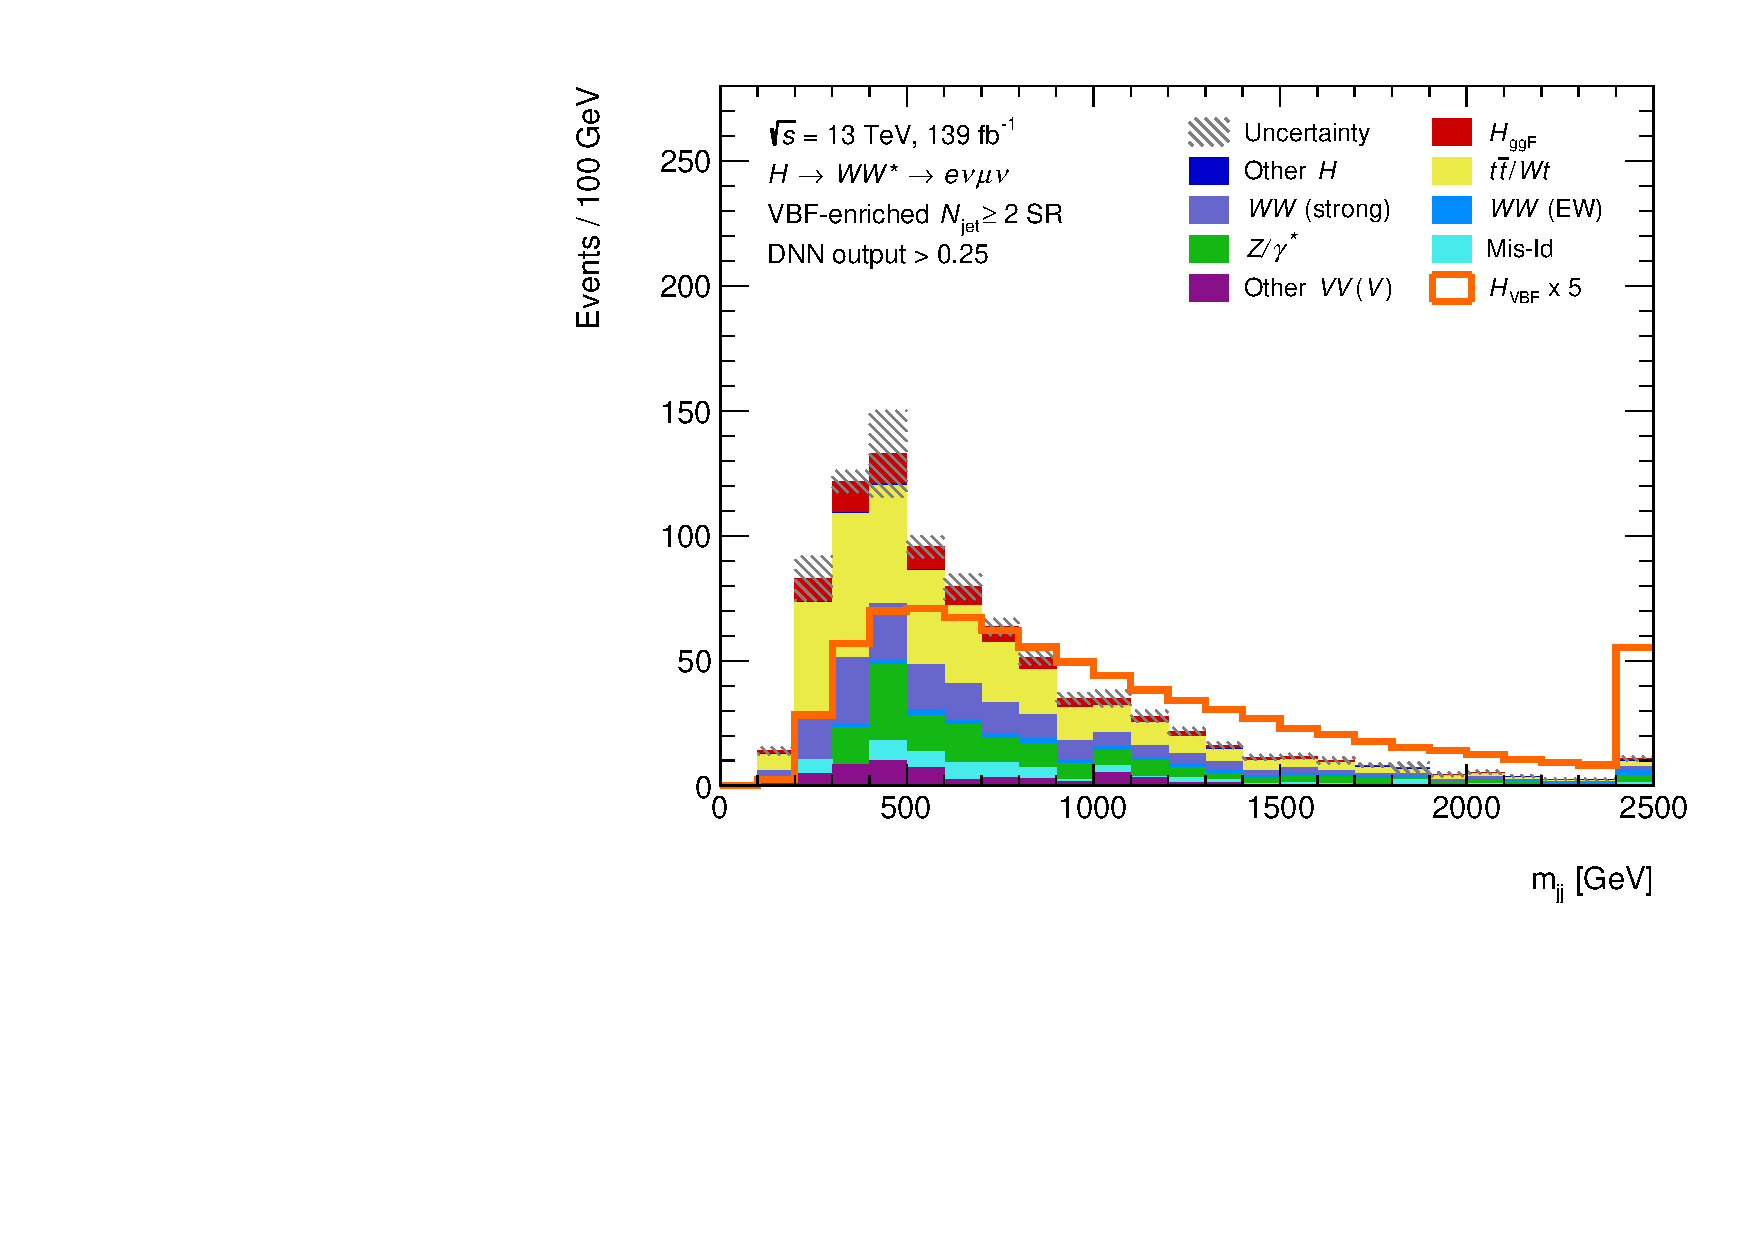
\includegraphics[width=0.32\textwidth]{figures/hww/dnn/blinded/run2-emme-CutVBFSR_DNN25-Mjj-lin.pdf} \hfill
        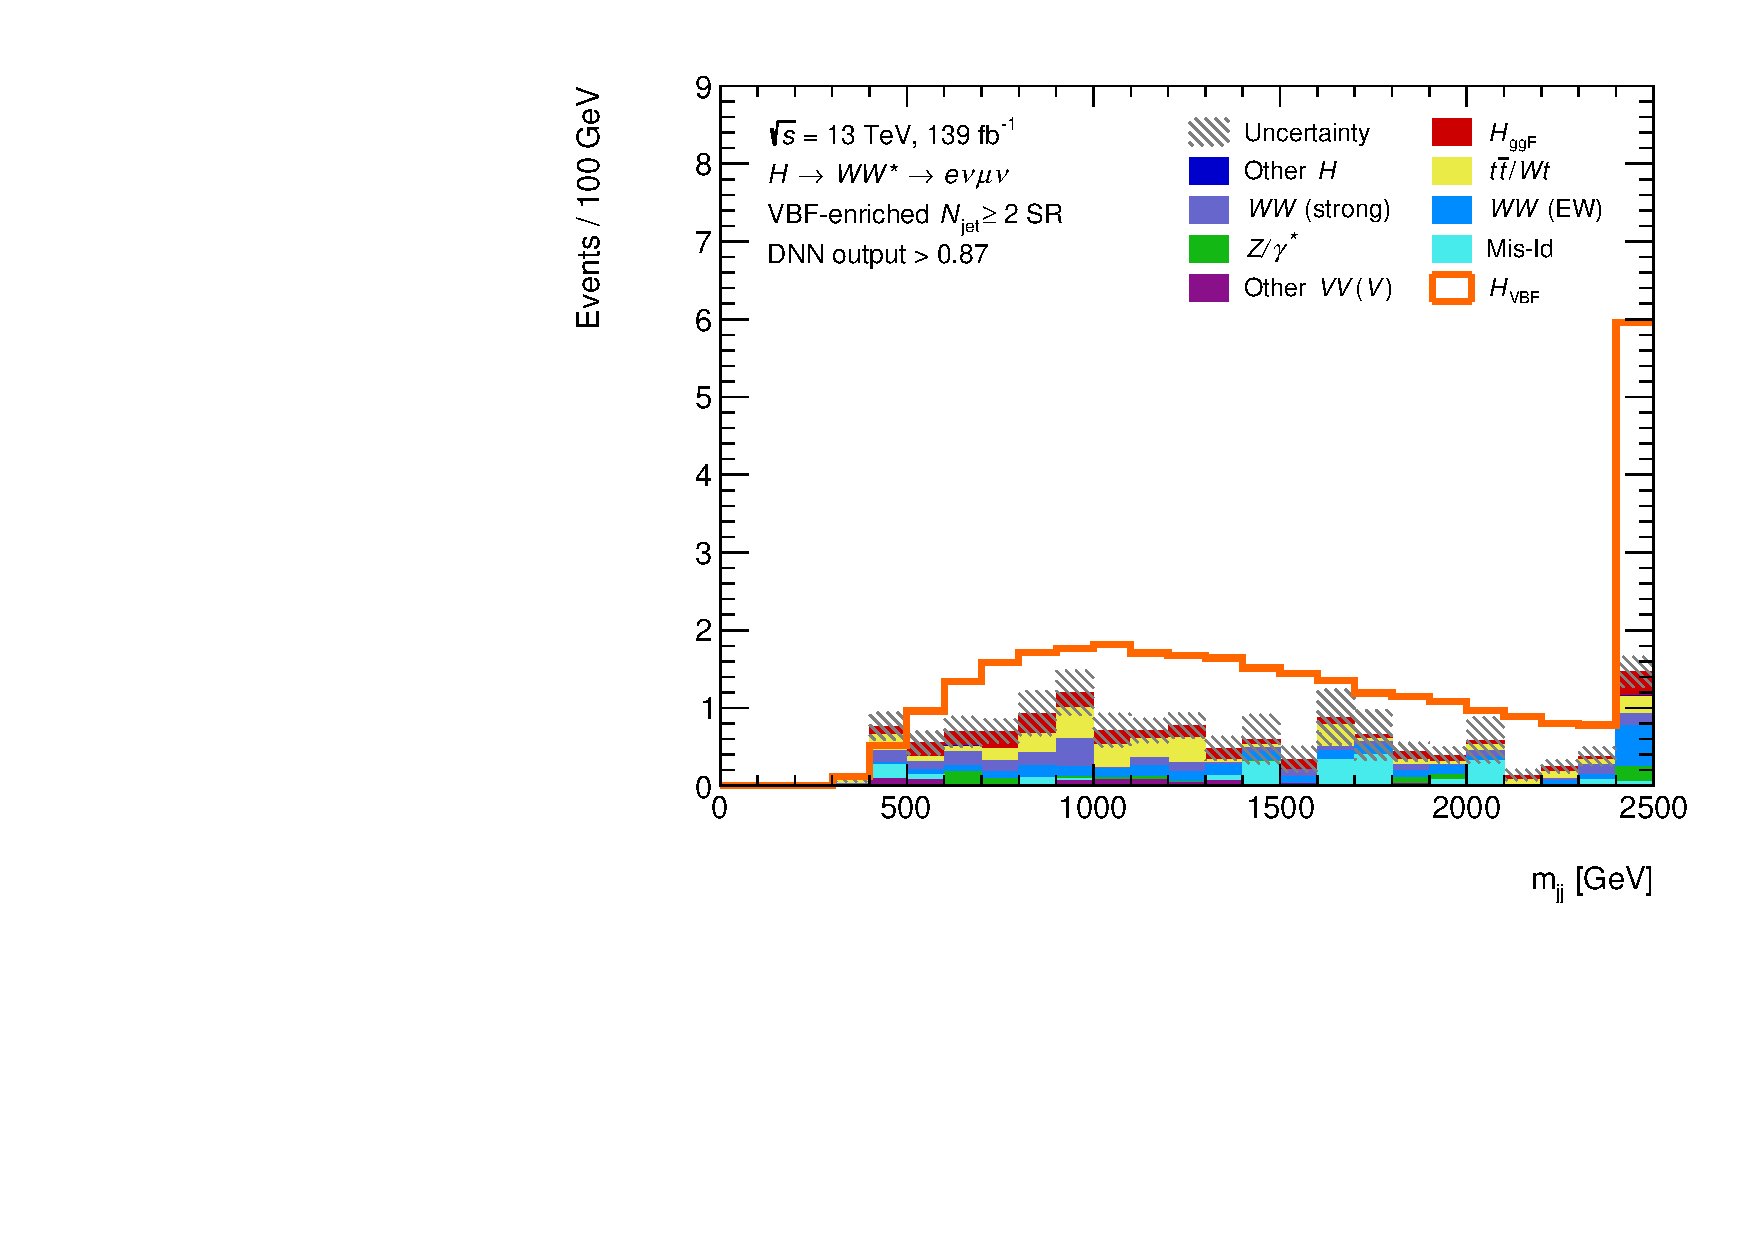
\includegraphics[width=0.32\textwidth]{figures/hww/dnn/blinded/run2-emme-CutVBFSR_DNN87-Mjj-lin.pdf}
    } \\
    \subfloat[$\dyjj$]{
        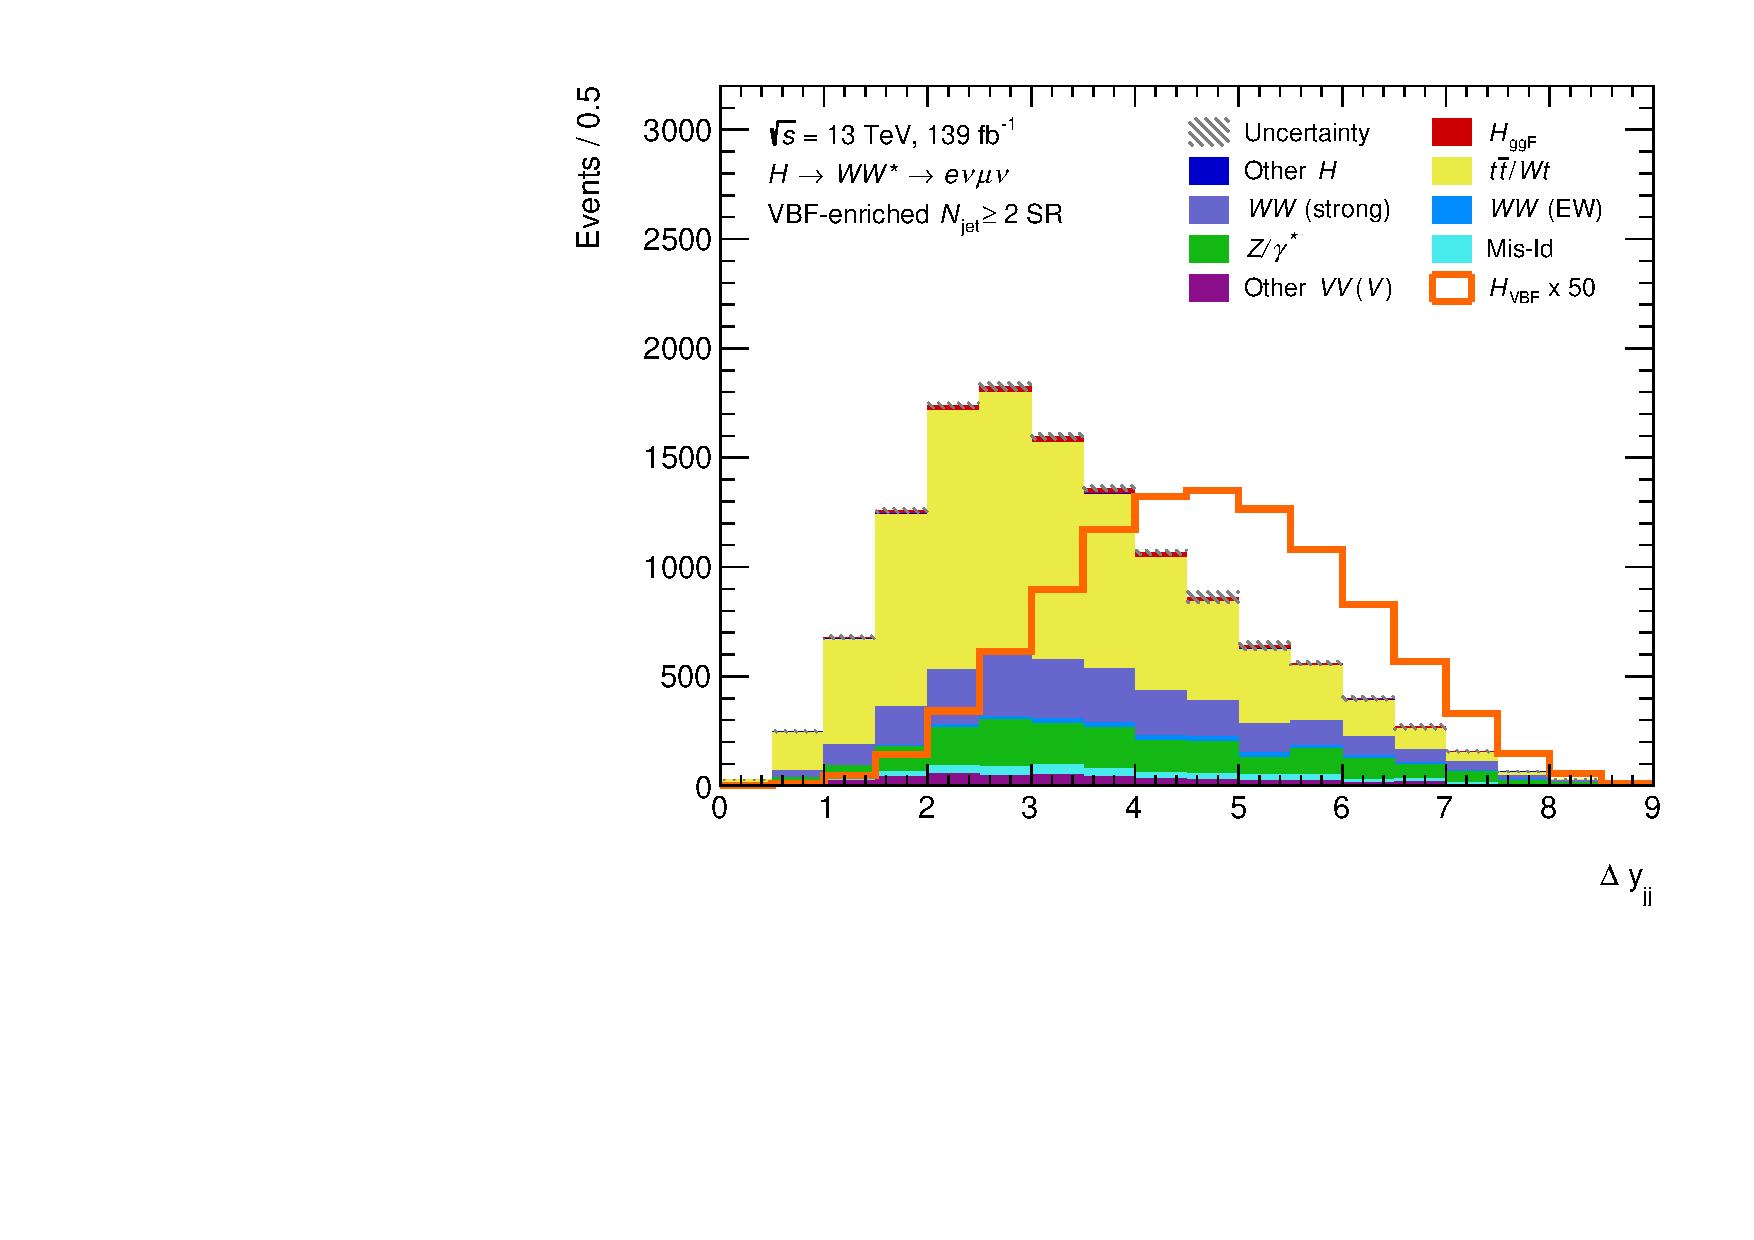
\includegraphics[width=0.32\textwidth]{figures/hww/dnn/blinded/run2-emme-CutVBF_SR-DYjj-lin.pdf} \hfill
        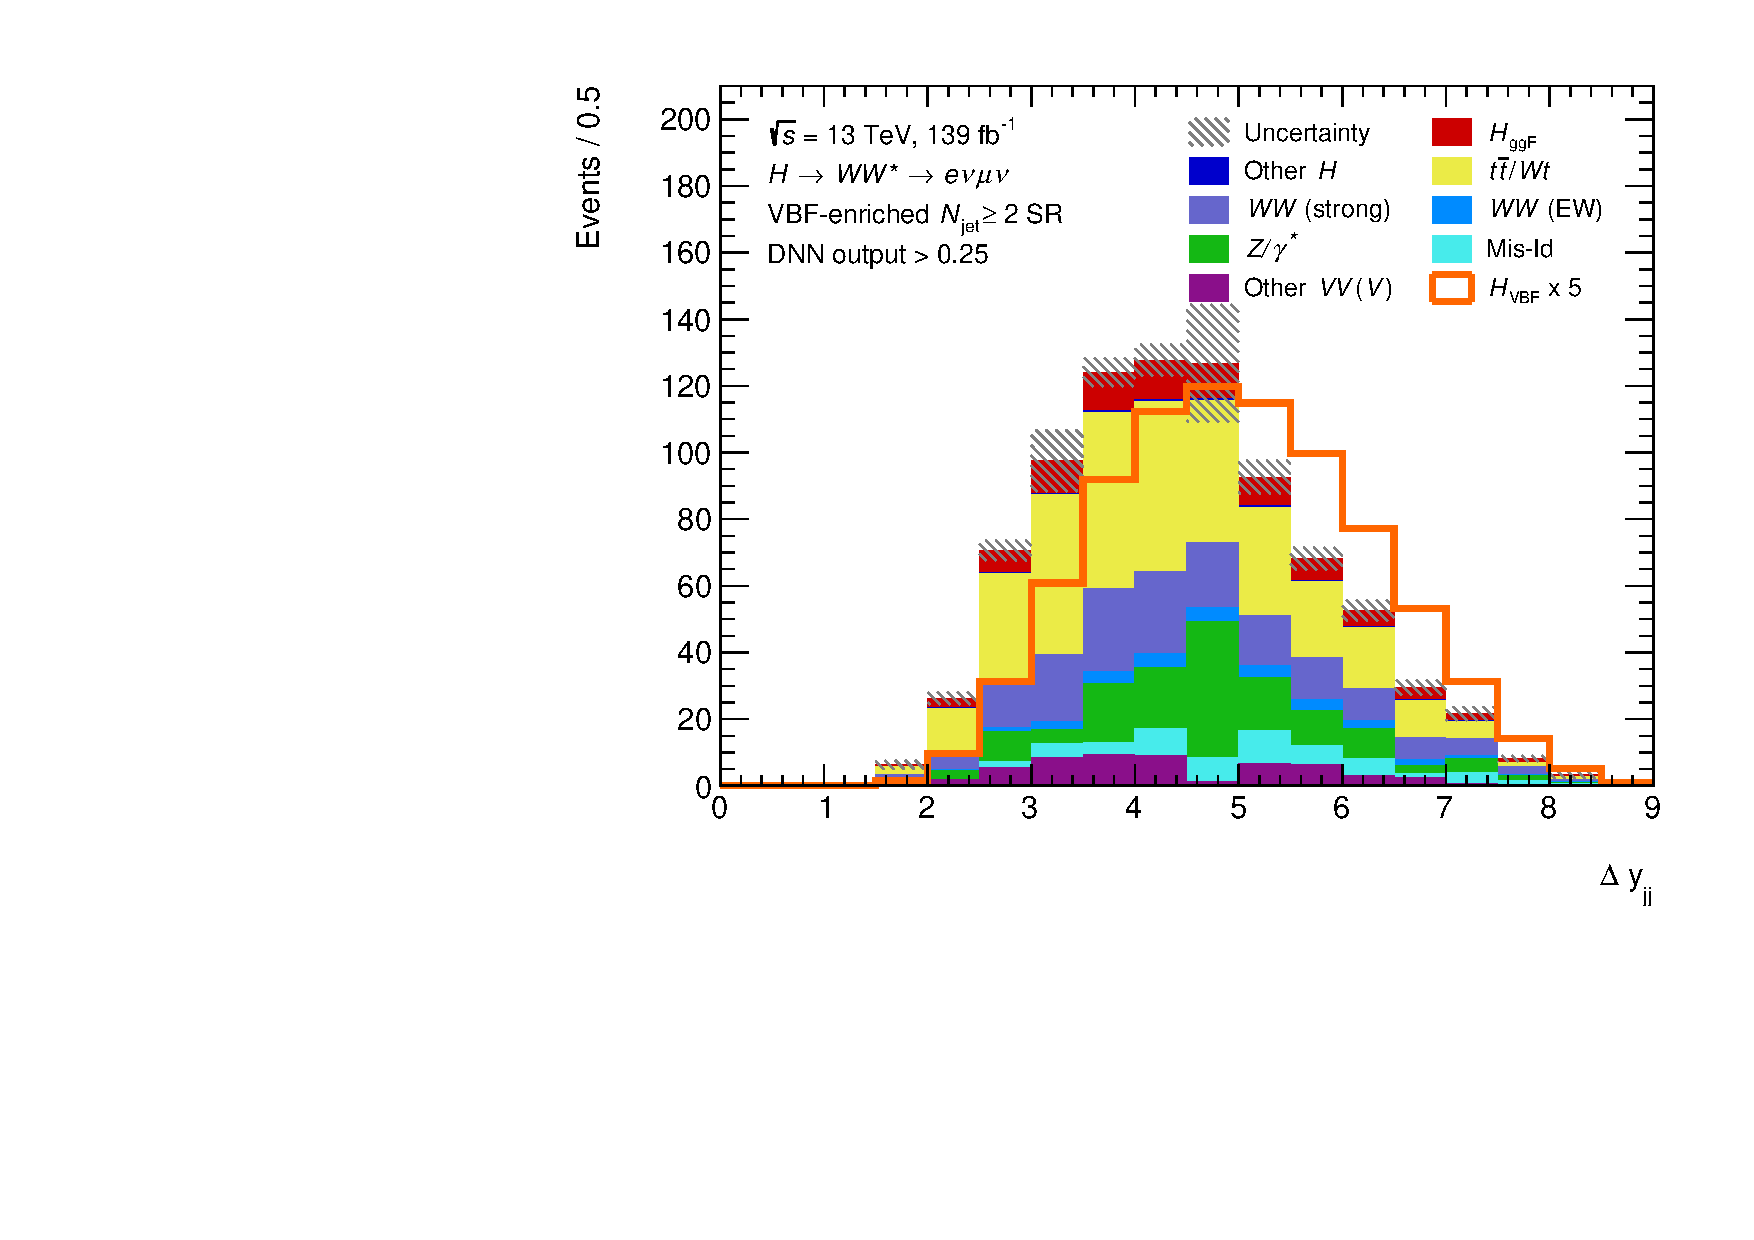
\includegraphics[width=0.32\textwidth]{figures/hww/dnn/blinded/run2-emme-CutVBFSR_DNN25-DYjj-lin.pdf} \hfill
        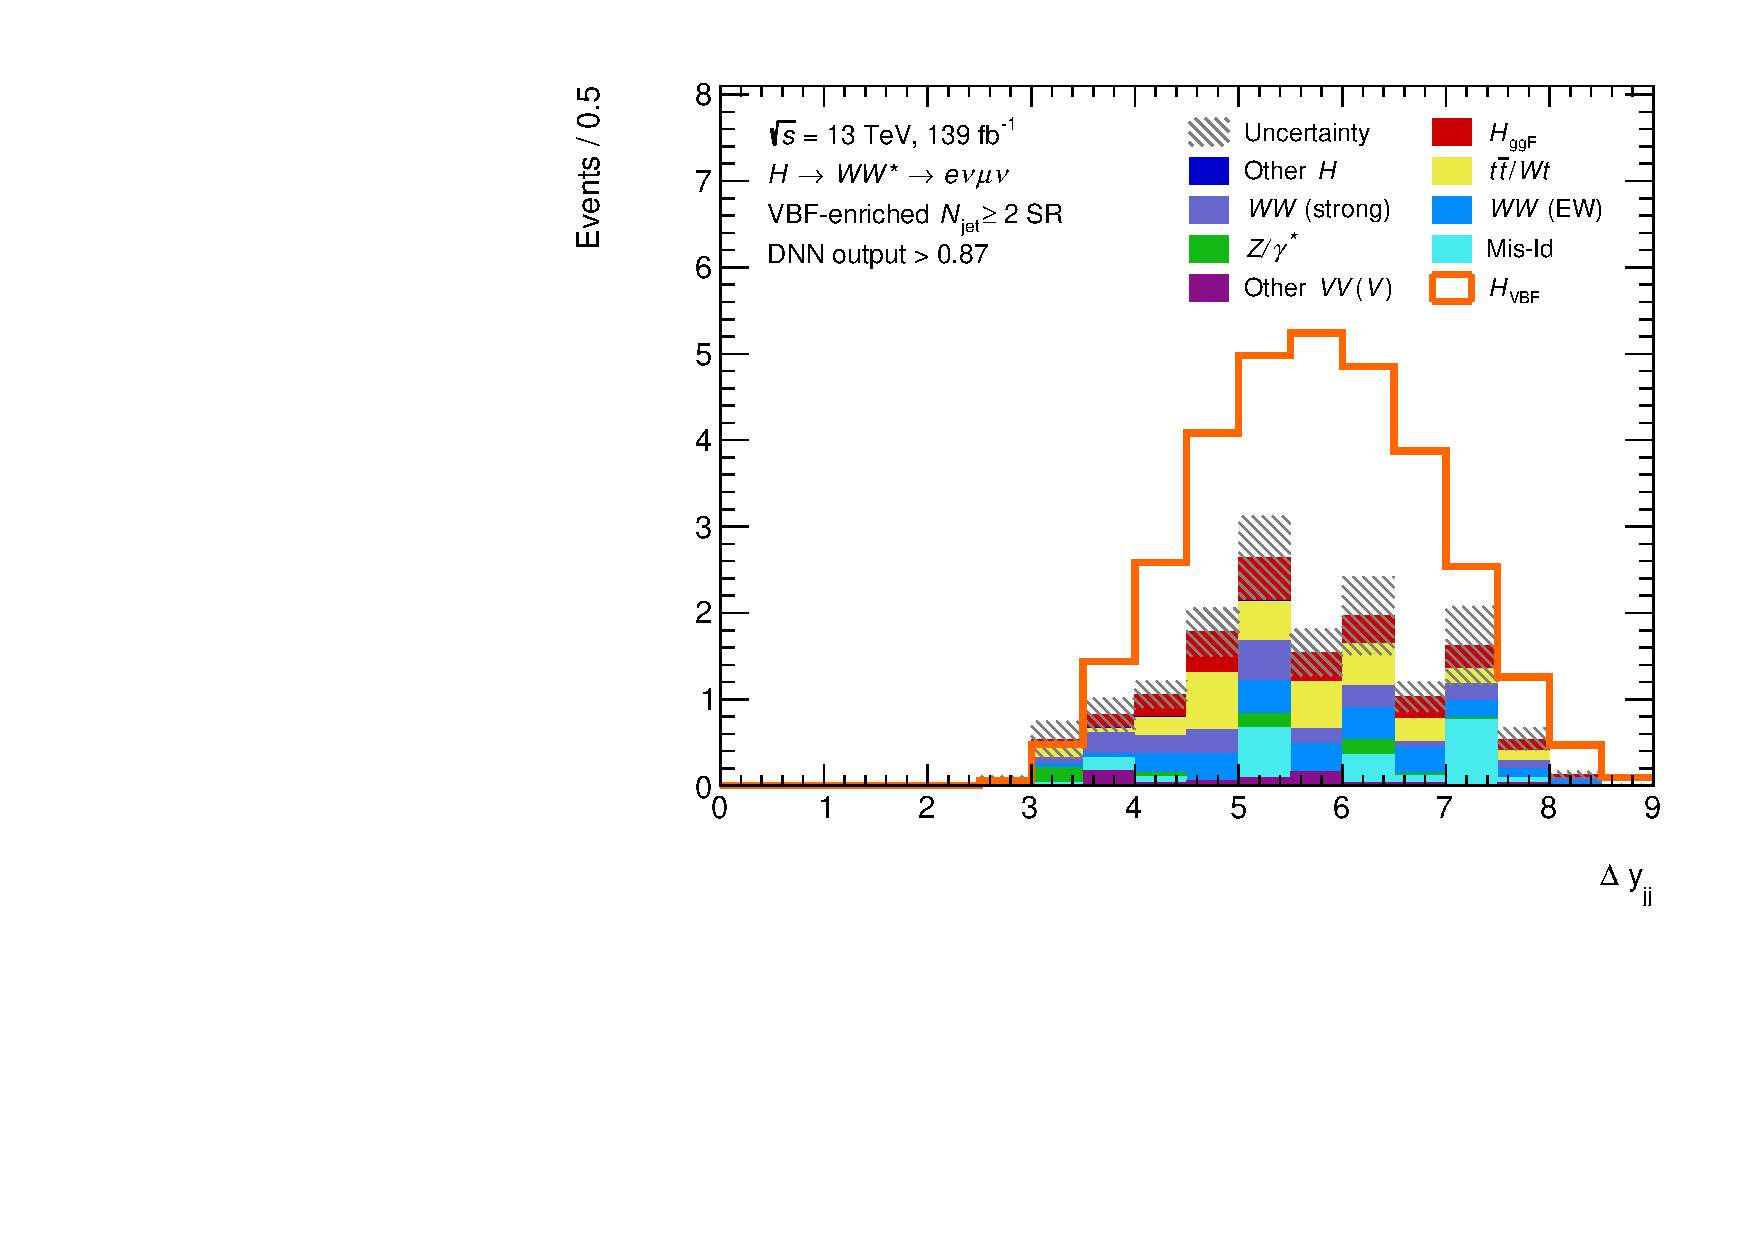
\includegraphics[width=0.32\textwidth]{figures/hww/dnn/blinded/run2-emme-CutVBFSR_DNN87-DYjj-lin.pdf}
    } \\
    \subfloat[$\lepetacent$]{
        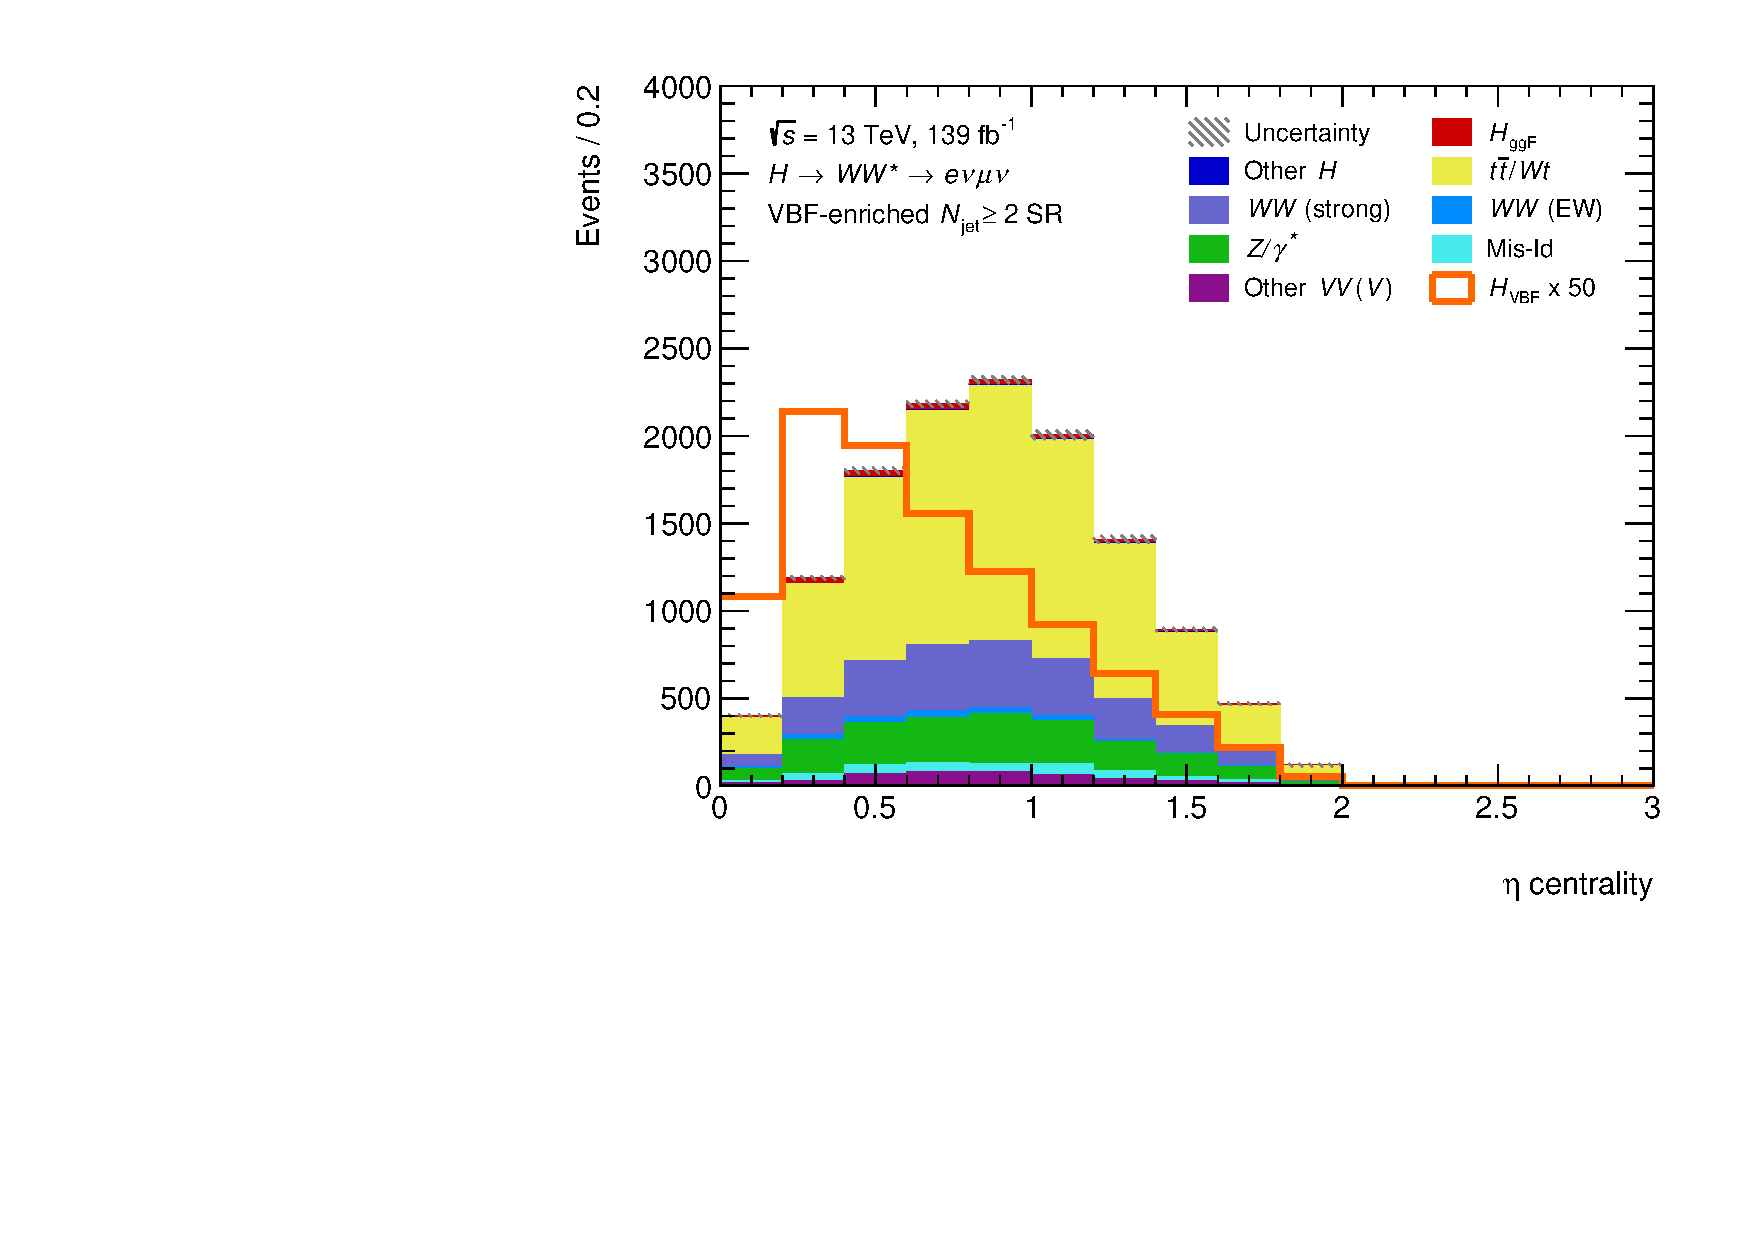
\includegraphics[width=0.32\textwidth]{figures/hww/dnn/blinded/run2-emme-CutVBF_SR-contOLV-lin.pdf} \hfill
        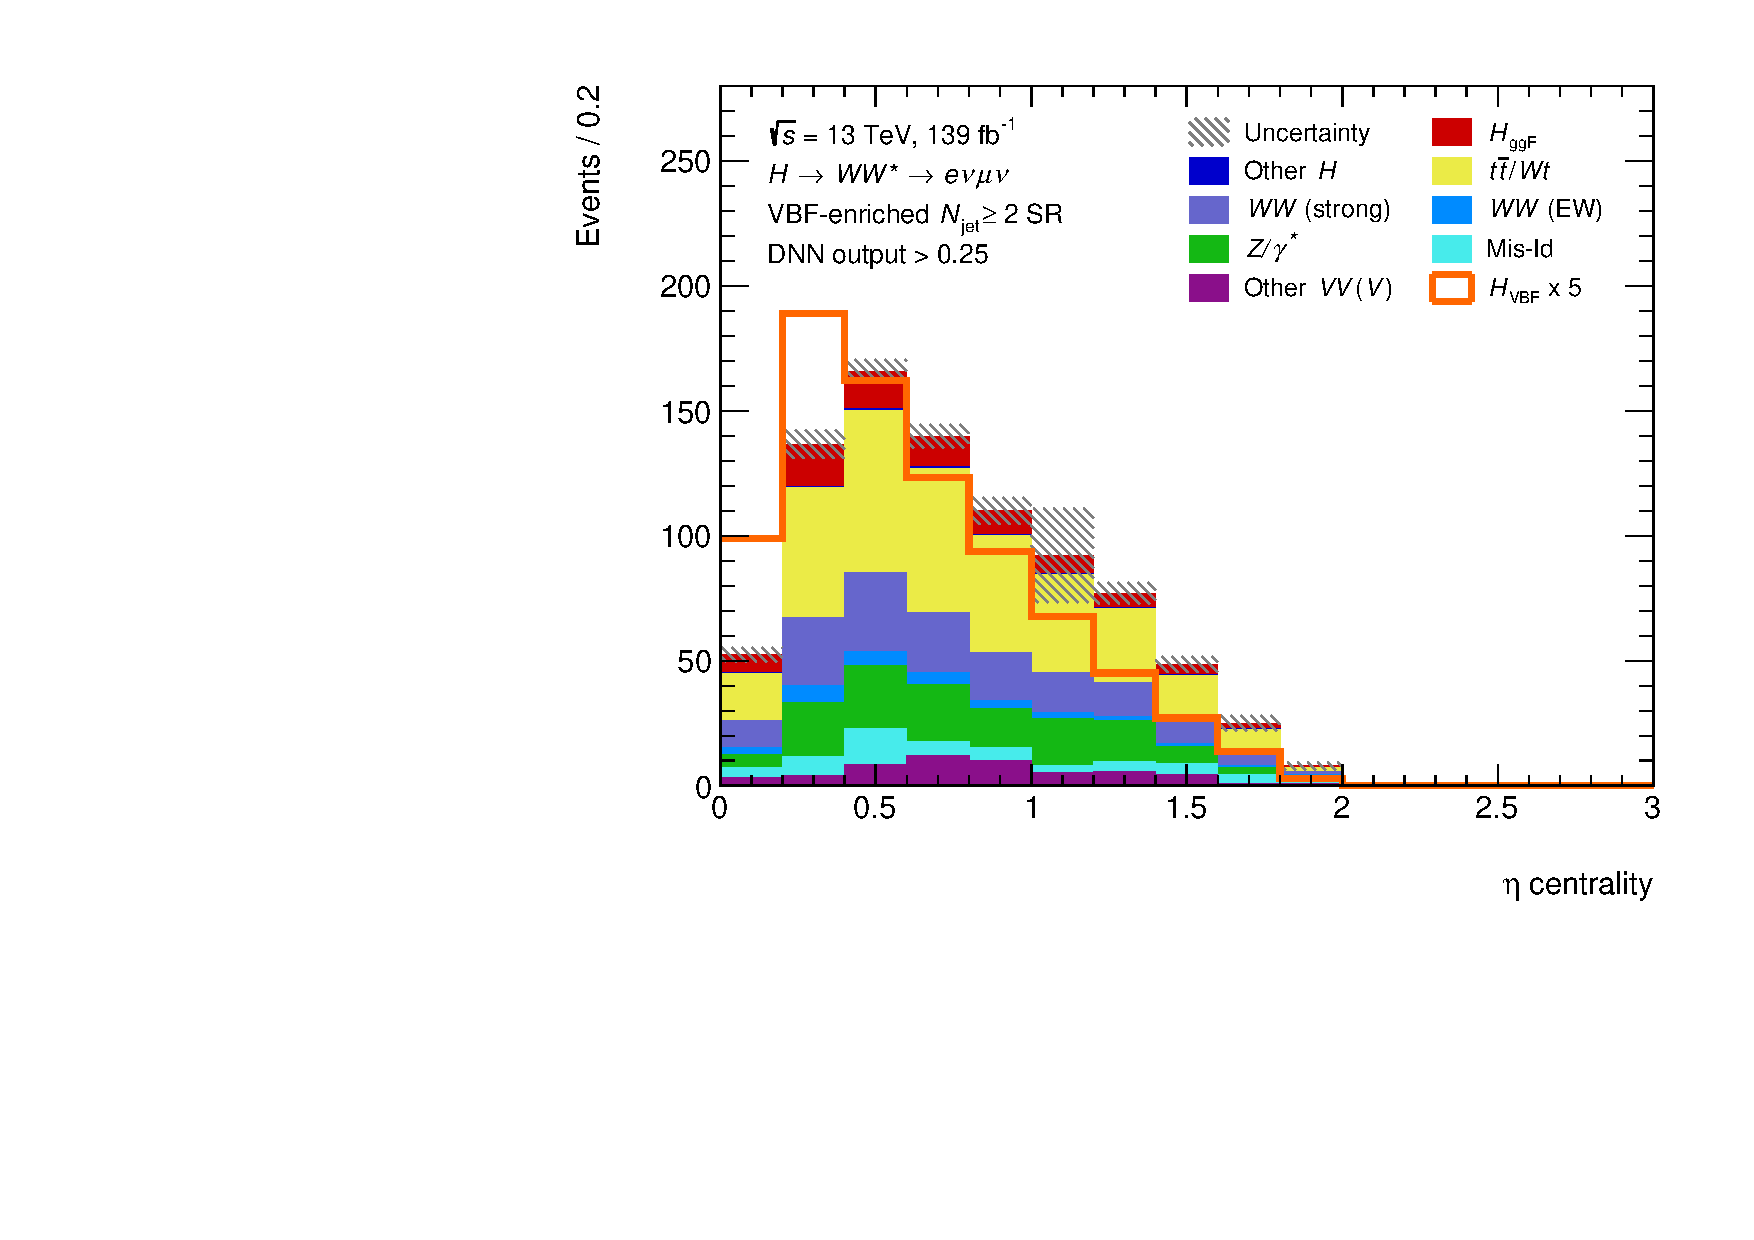
\includegraphics[width=0.32\textwidth]{figures/hww/dnn/blinded/run2-emme-CutVBFSR_DNN25-contOLV-lin.pdf} \hfill
        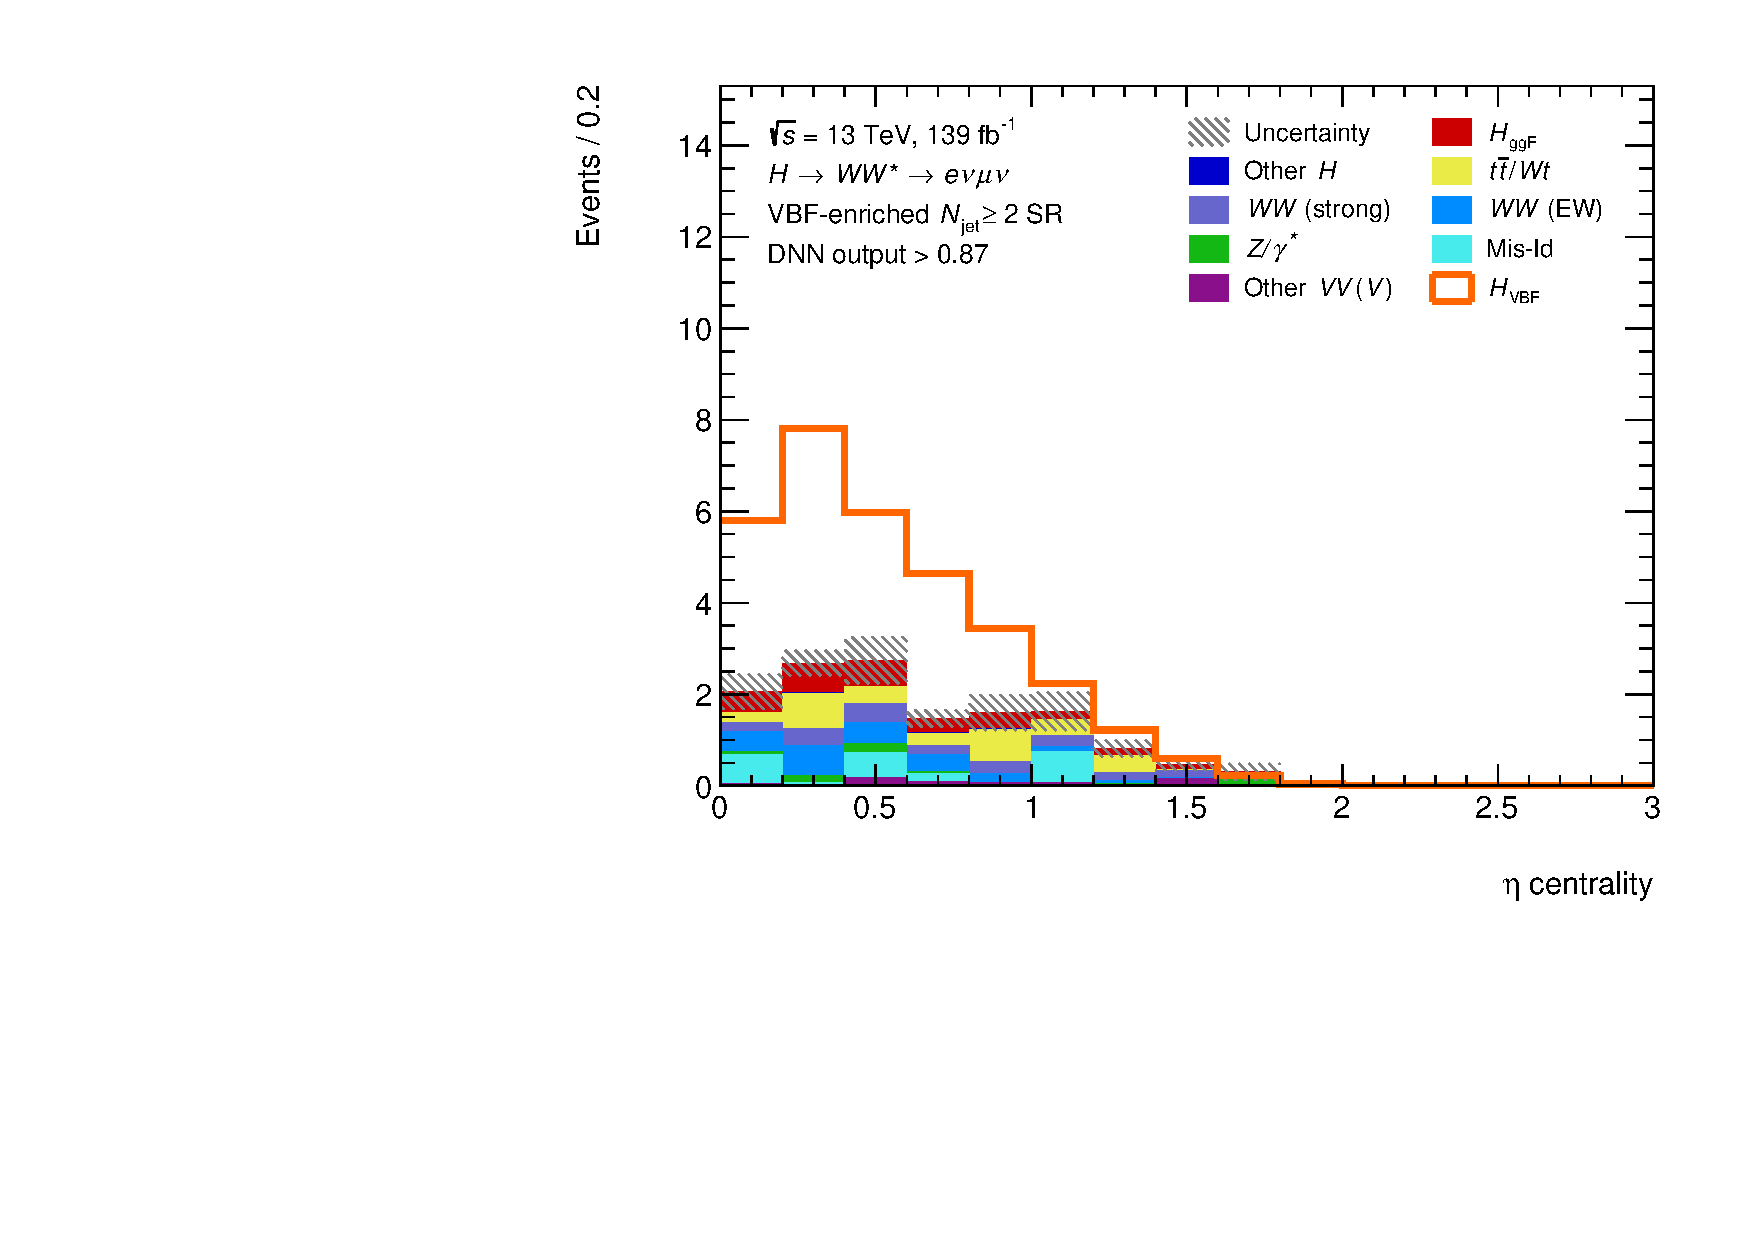
\includegraphics[width=0.32\textwidth]{figures/hww/dnn/blinded/run2-emme-CutVBFSR_DNN87-contOLV-lin.pdf}
    } \\
    {\caption{Distributions of $\dphill$, $\mll$, $\lepetacent$ in the VBF signal region.
        Each row corresponds to one variable with different selections made on the DNN output.
        \label{app:fig:dnn-inputs-vbf-top1} }}
\end{figure}


\begin{figure}[h]
    \centering
    \subfloat[$\mlonejtwo$]{
        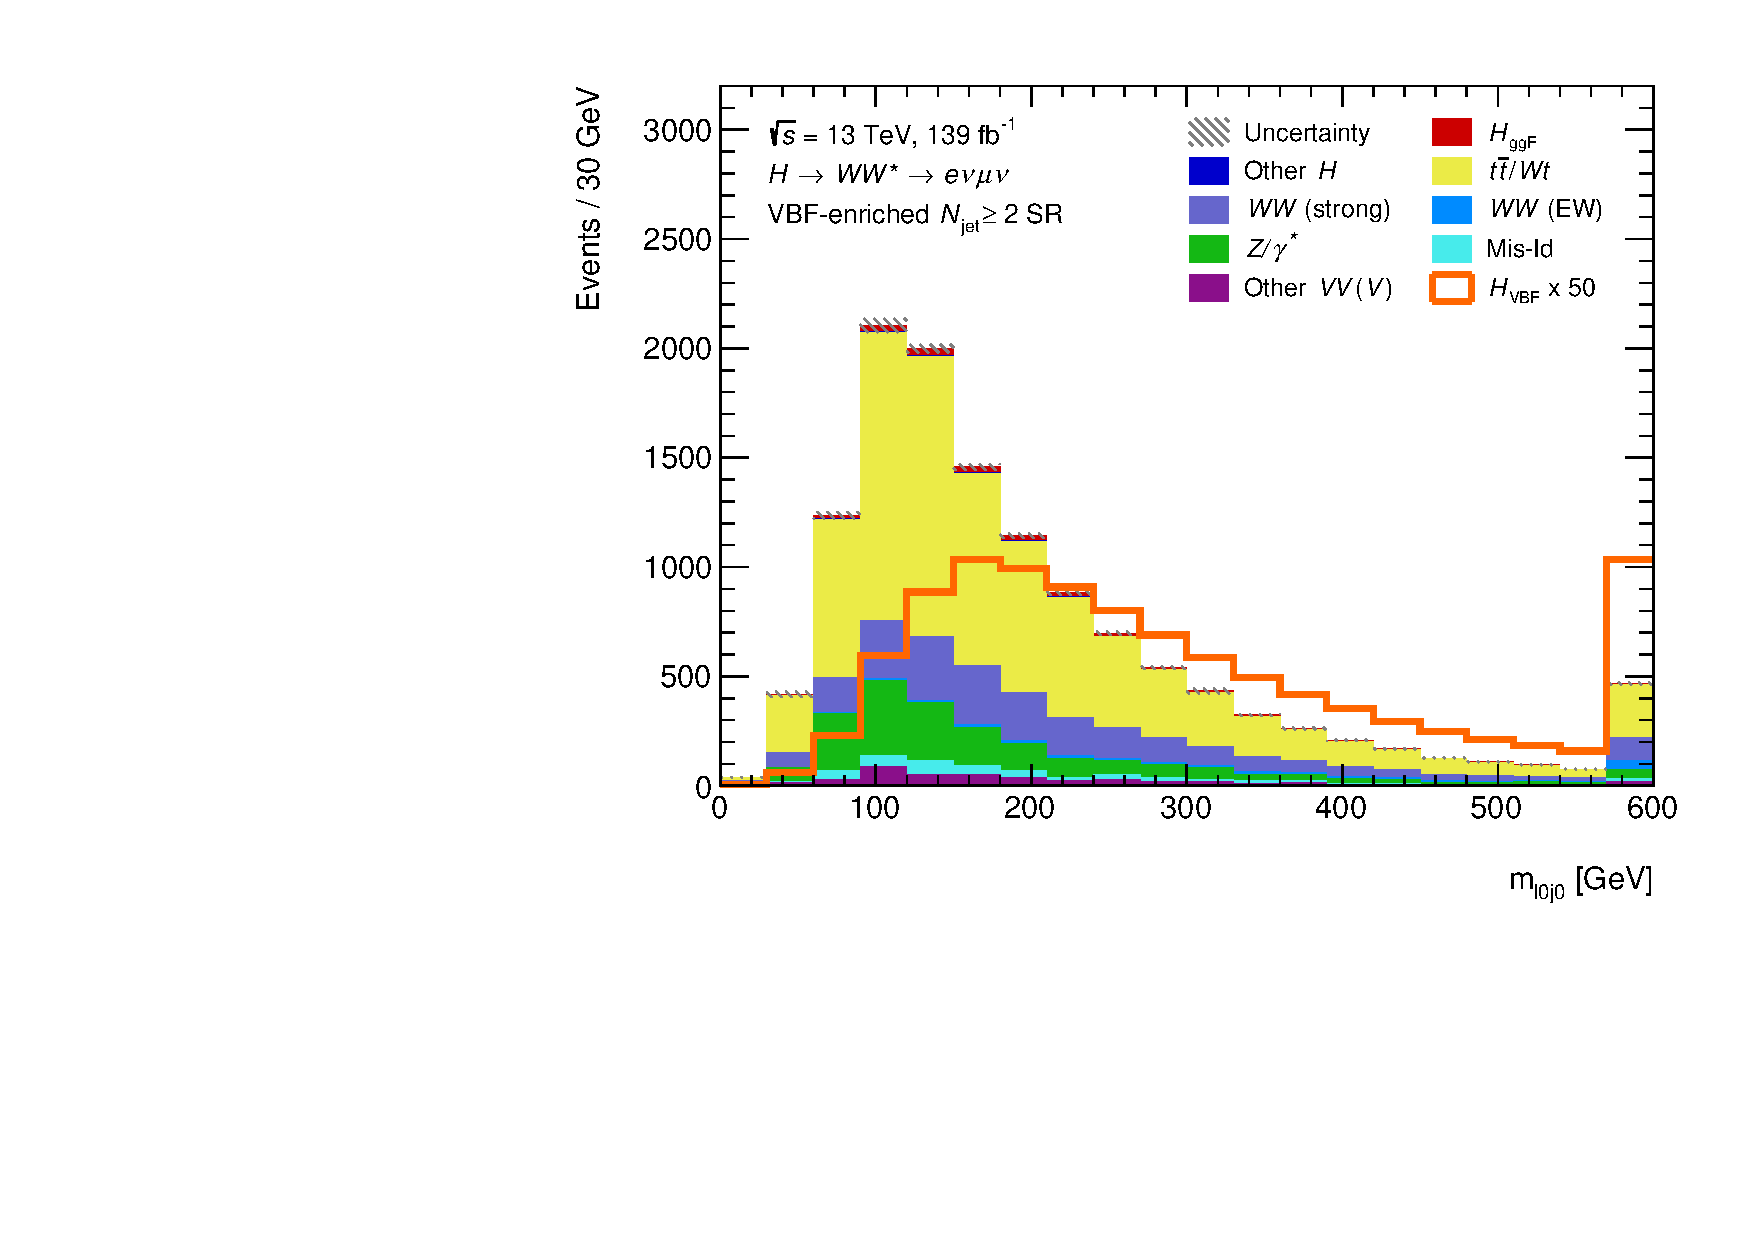
\includegraphics[width=0.32\textwidth]{figures/hww/dnn/blinded/run2-emme-CutVBF_SR-Ml0j0-lin.pdf} \hfill
        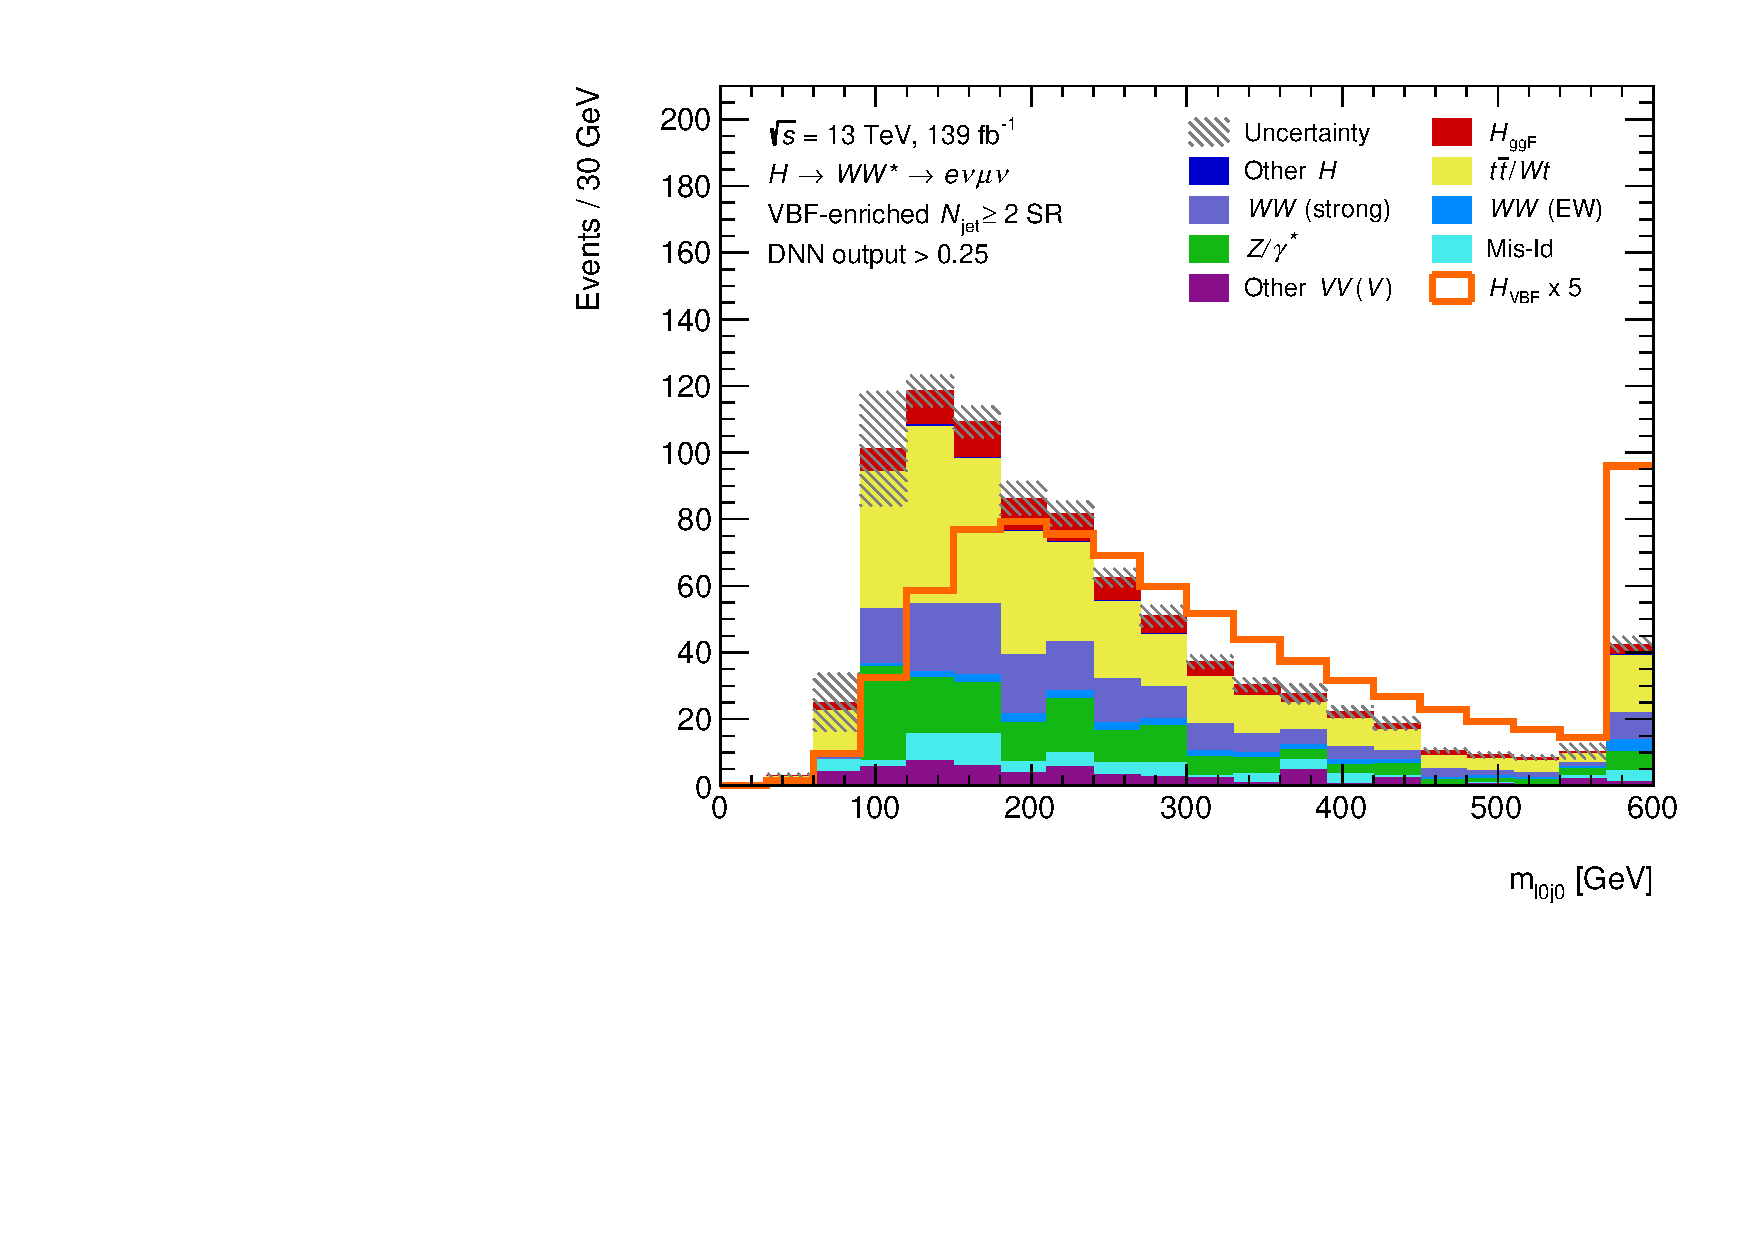
\includegraphics[width=0.32\textwidth]{figures/hww/dnn/blinded/run2-emme-CutVBFSR_DNN25-Ml0j0-lin.pdf} \hfill
        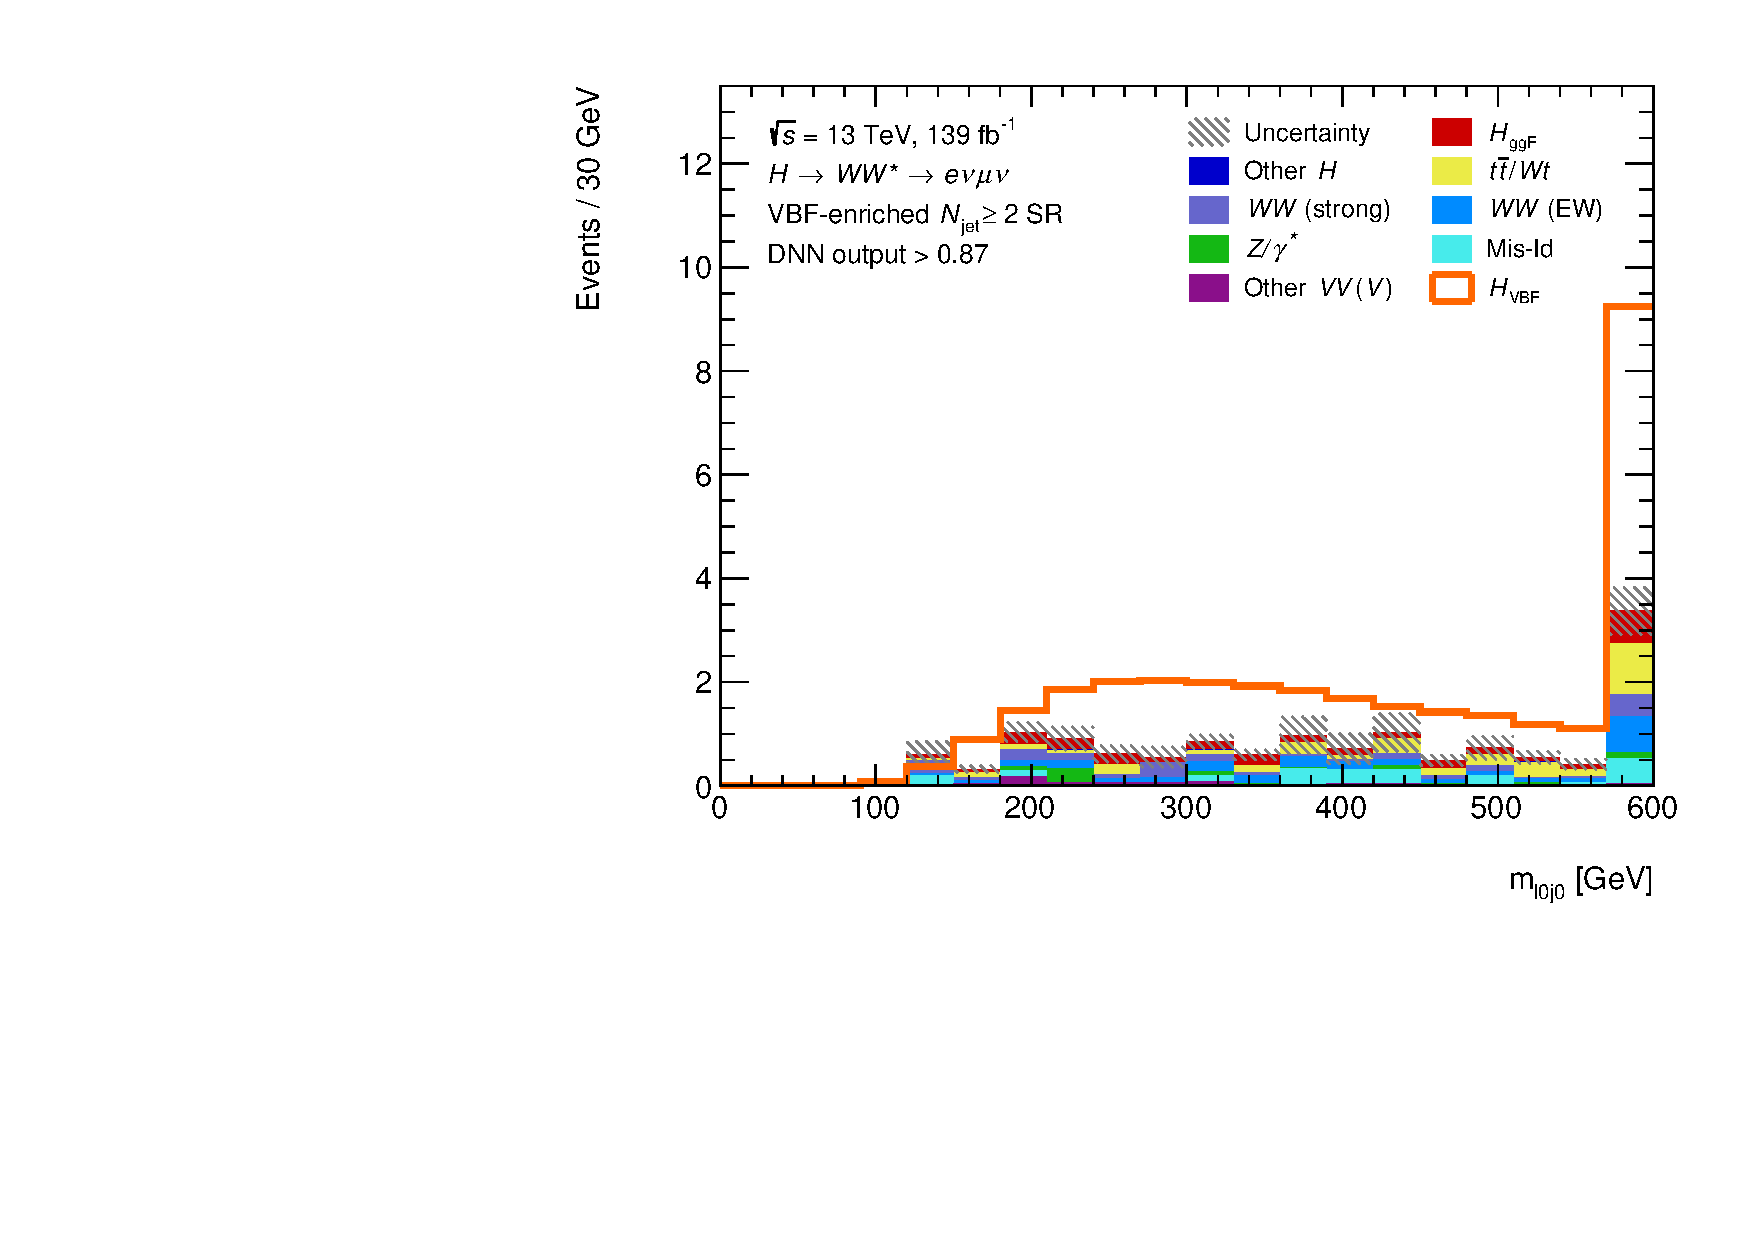
\includegraphics[width=0.32\textwidth]{figures/hww/dnn/blinded/run2-emme-CutVBFSR_DNN87-Ml0j0-lin.pdf}
    } \\
    \subfloat[$\mltwojone$]{
        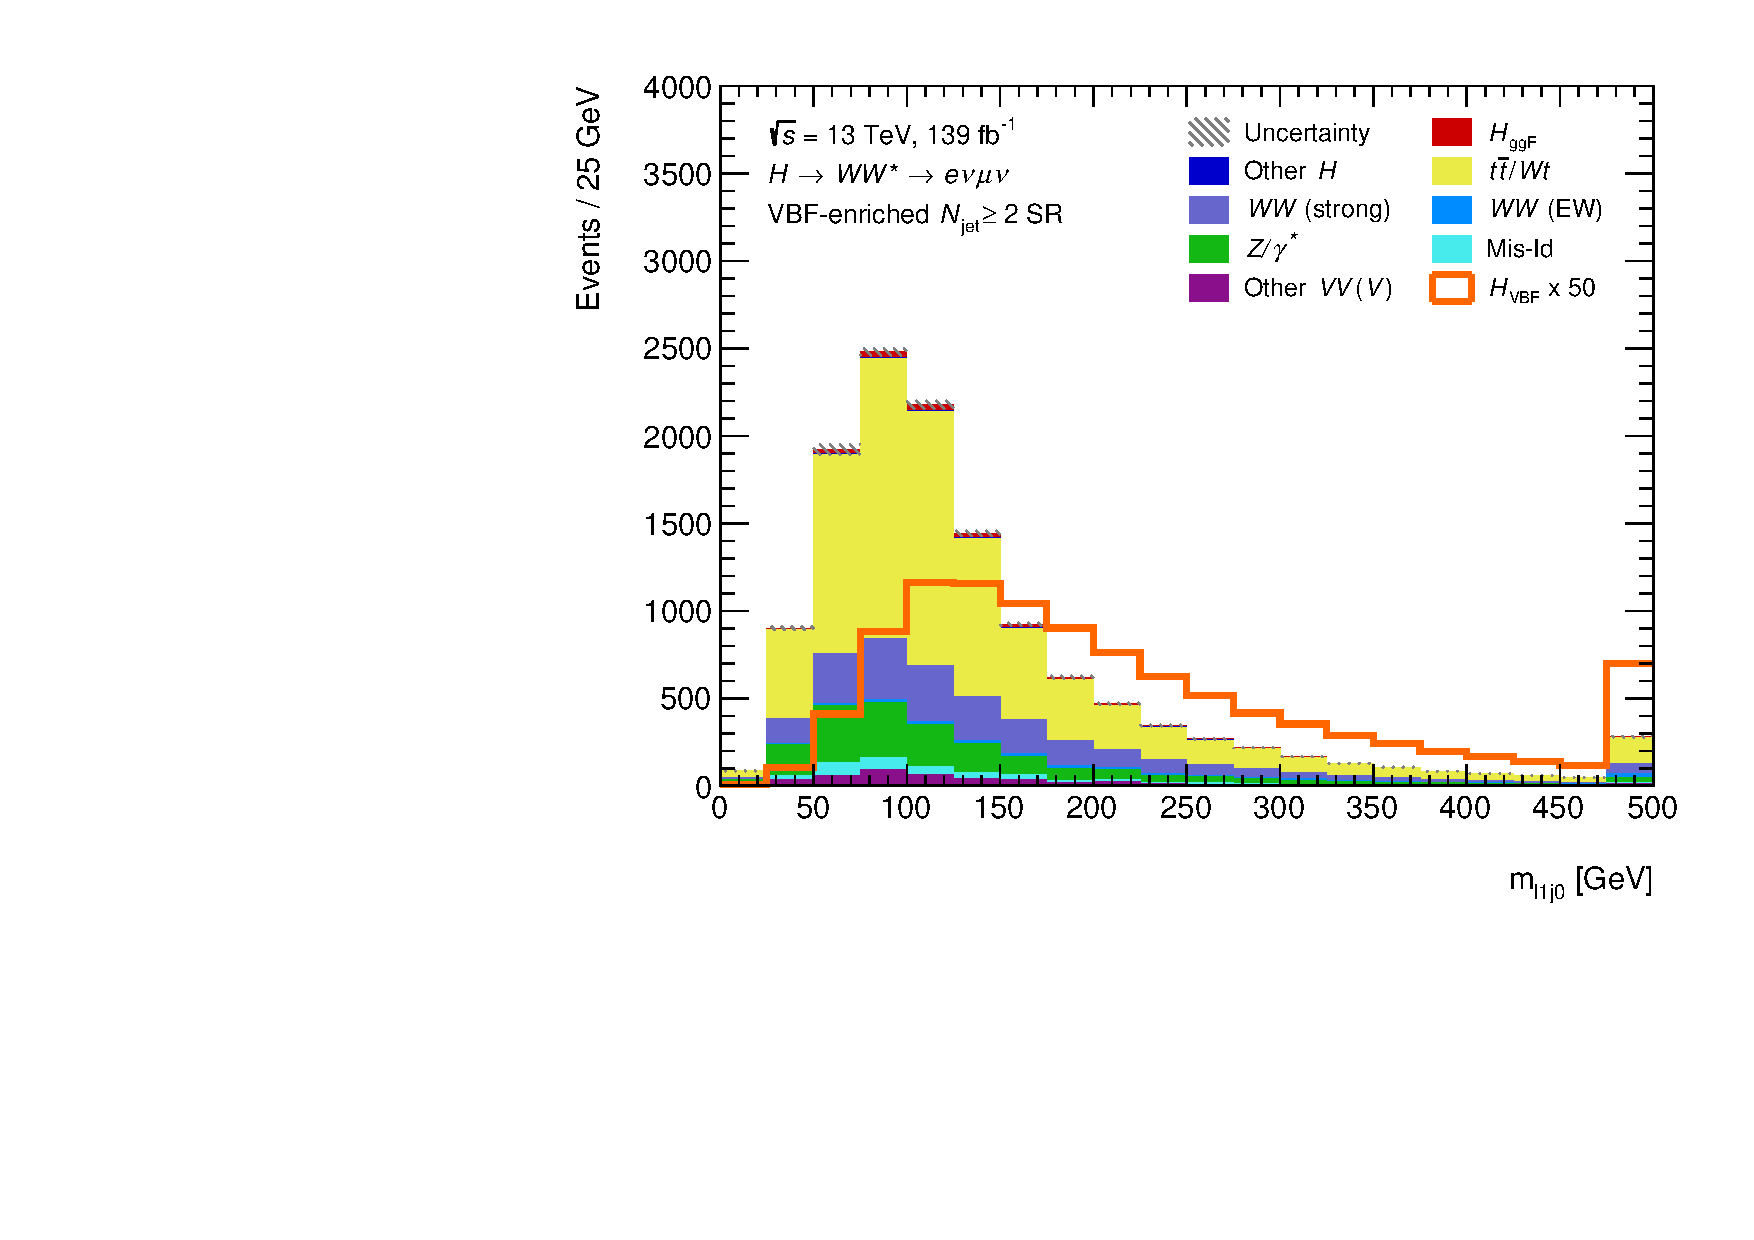
\includegraphics[width=0.32\textwidth]{figures/hww/dnn/blinded/run2-emme-CutVBF_SR-Ml1j0-lin.pdf} \hfill
        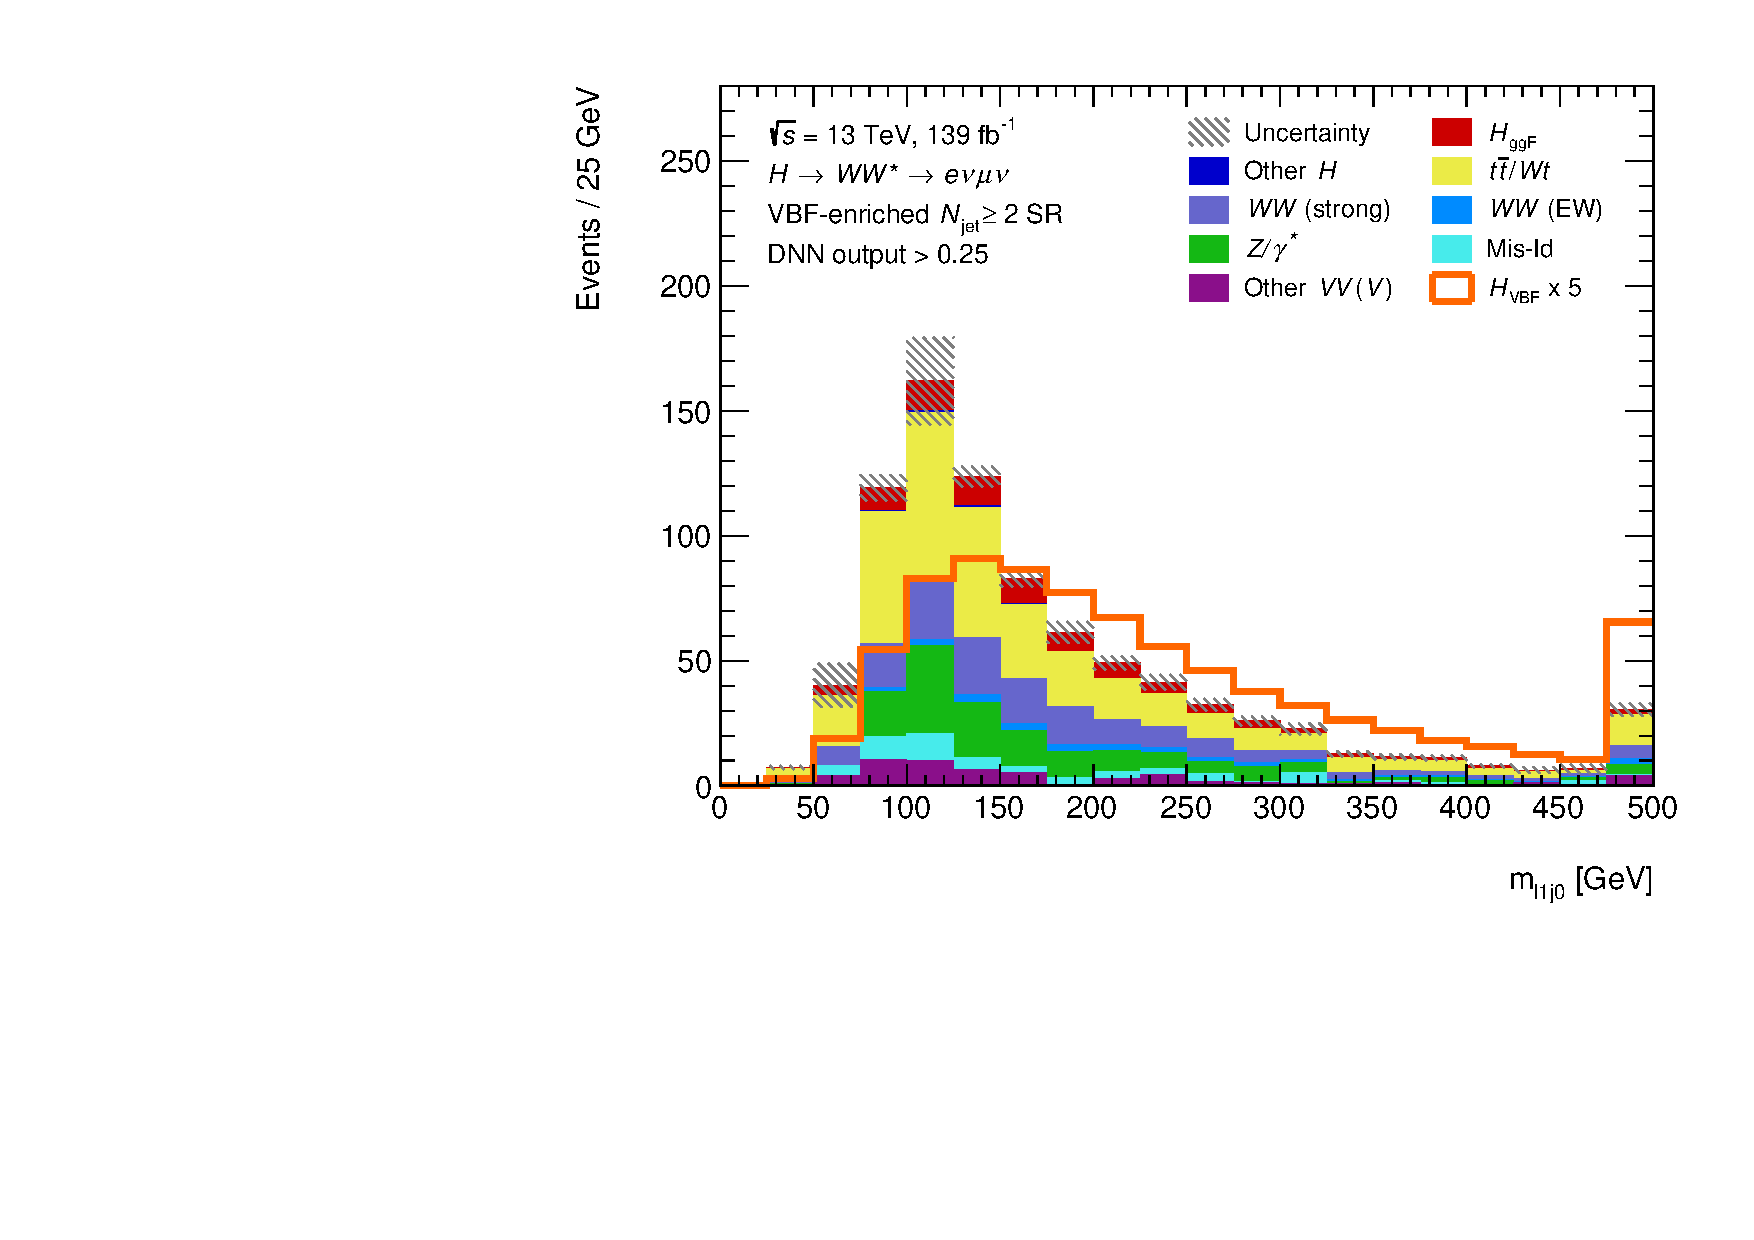
\includegraphics[width=0.32\textwidth]{figures/hww/dnn/blinded/run2-emme-CutVBFSR_DNN25-Ml1j0-lin.pdf} \hfill
        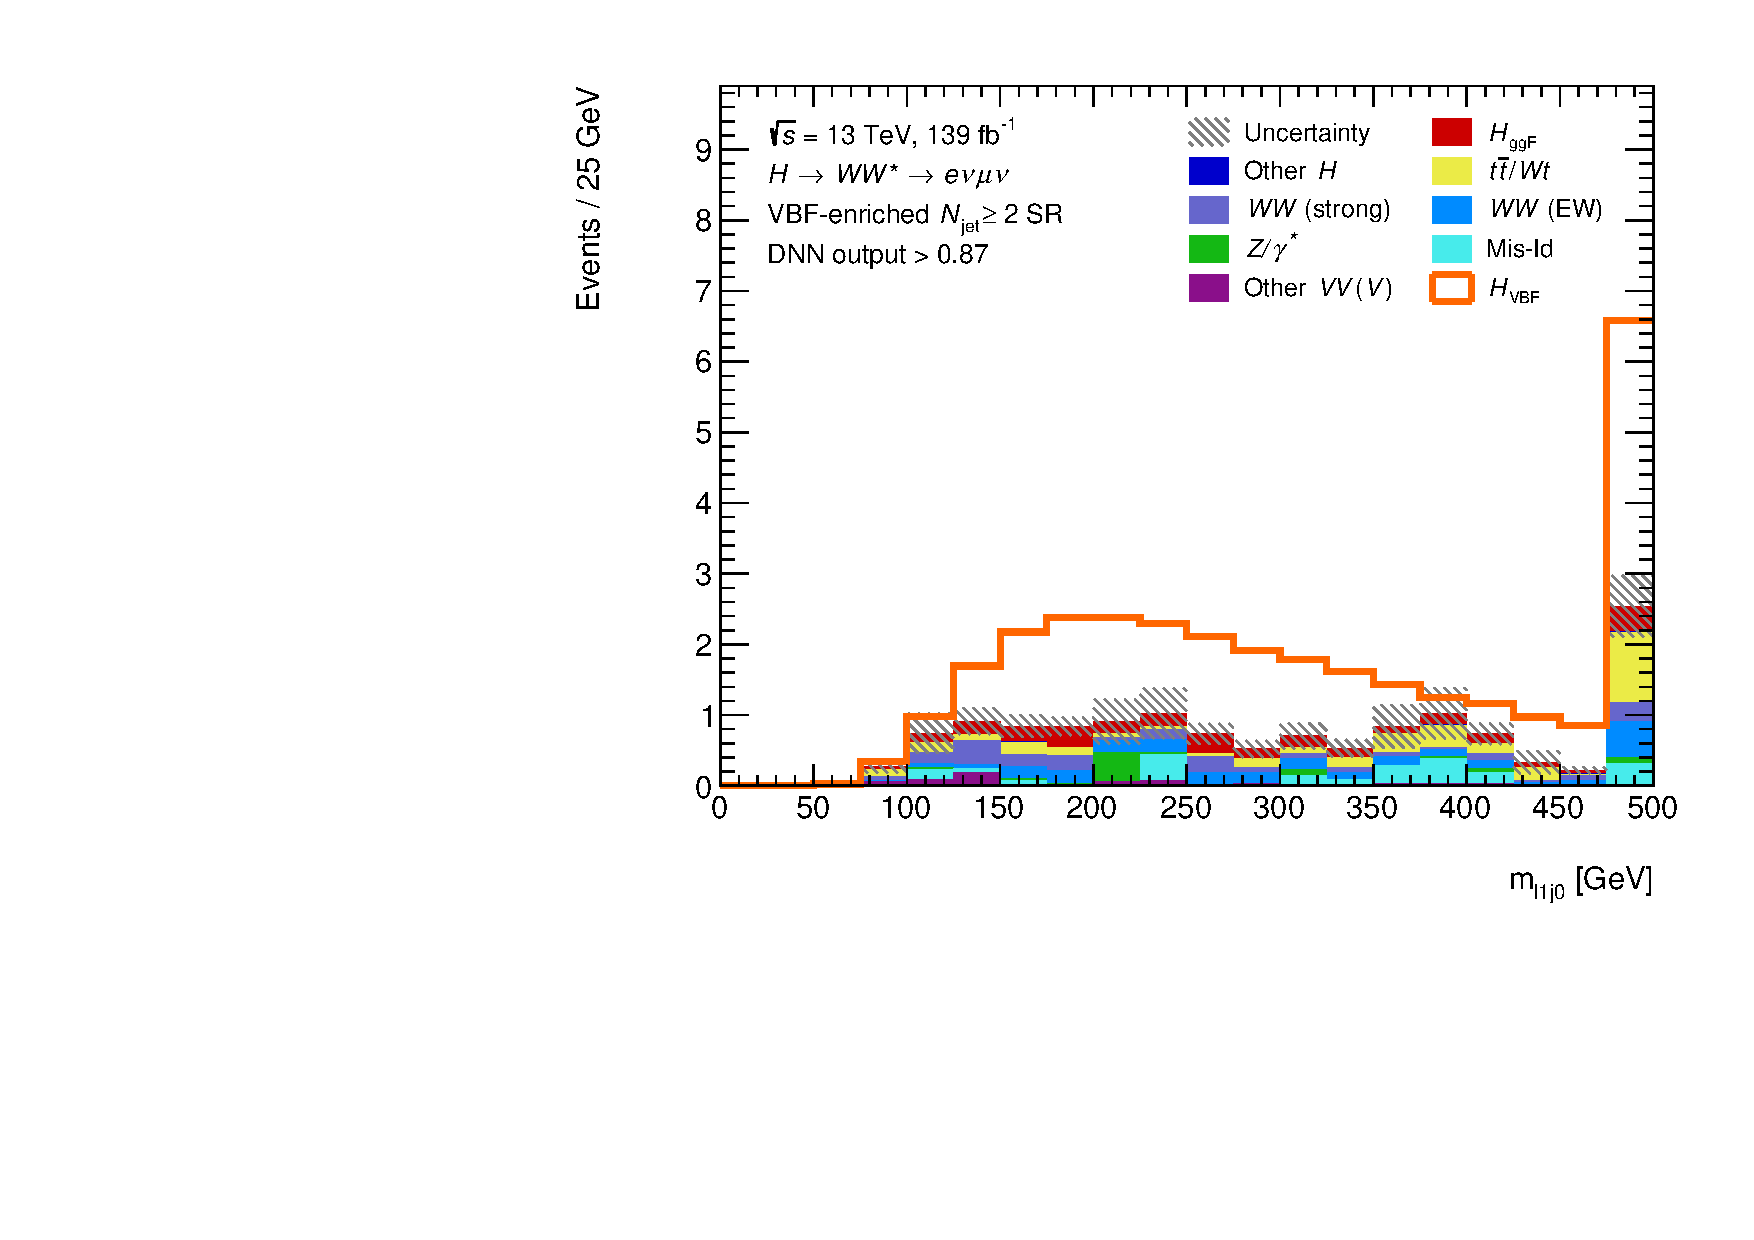
\includegraphics[width=0.32\textwidth]{figures/hww/dnn/blinded/run2-emme-CutVBFSR_DNN87-Ml1j0-lin.pdf}
    } \\
    \subfloat[$\mlonejtwo$]{
        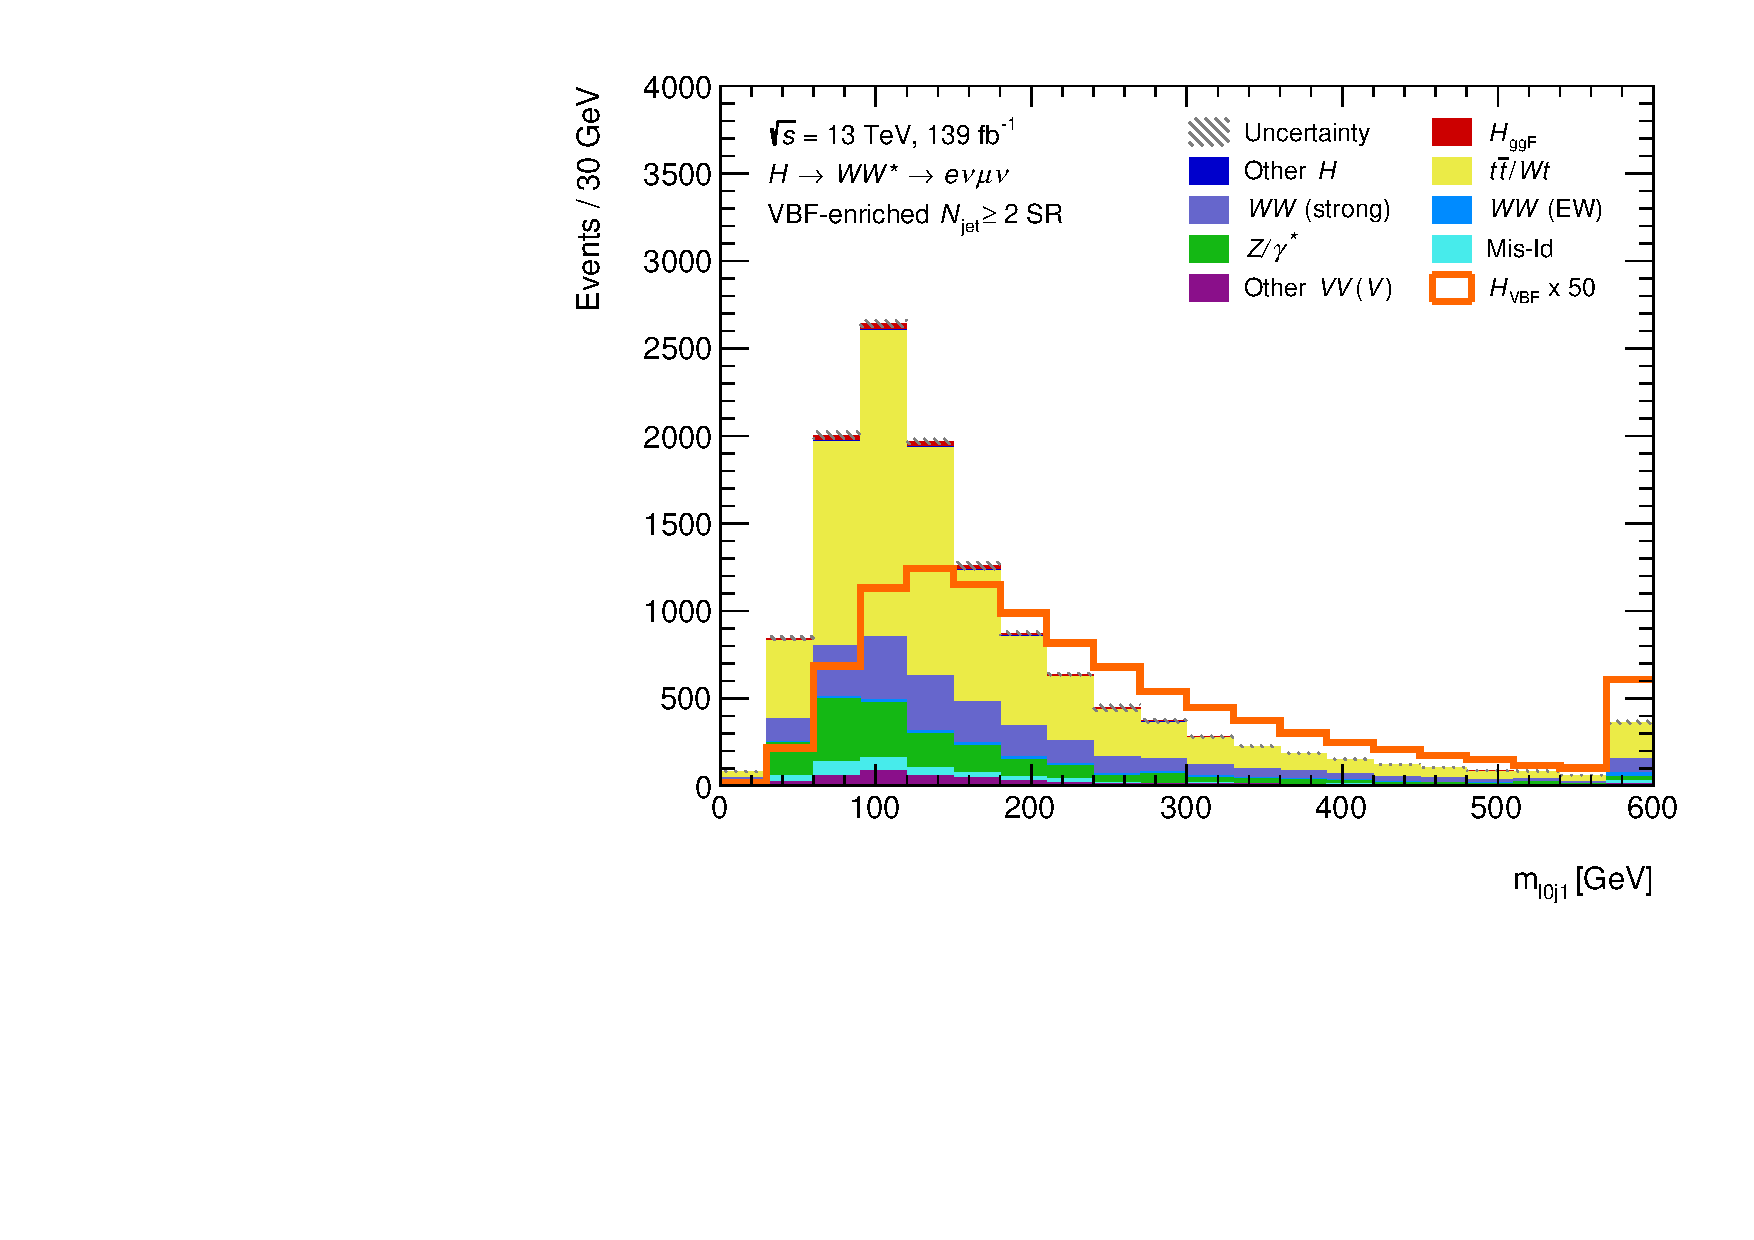
\includegraphics[width=0.32\textwidth]{figures/hww/dnn/blinded/run2-emme-CutVBF_SR-Ml0j1-lin.pdf} \hfill
        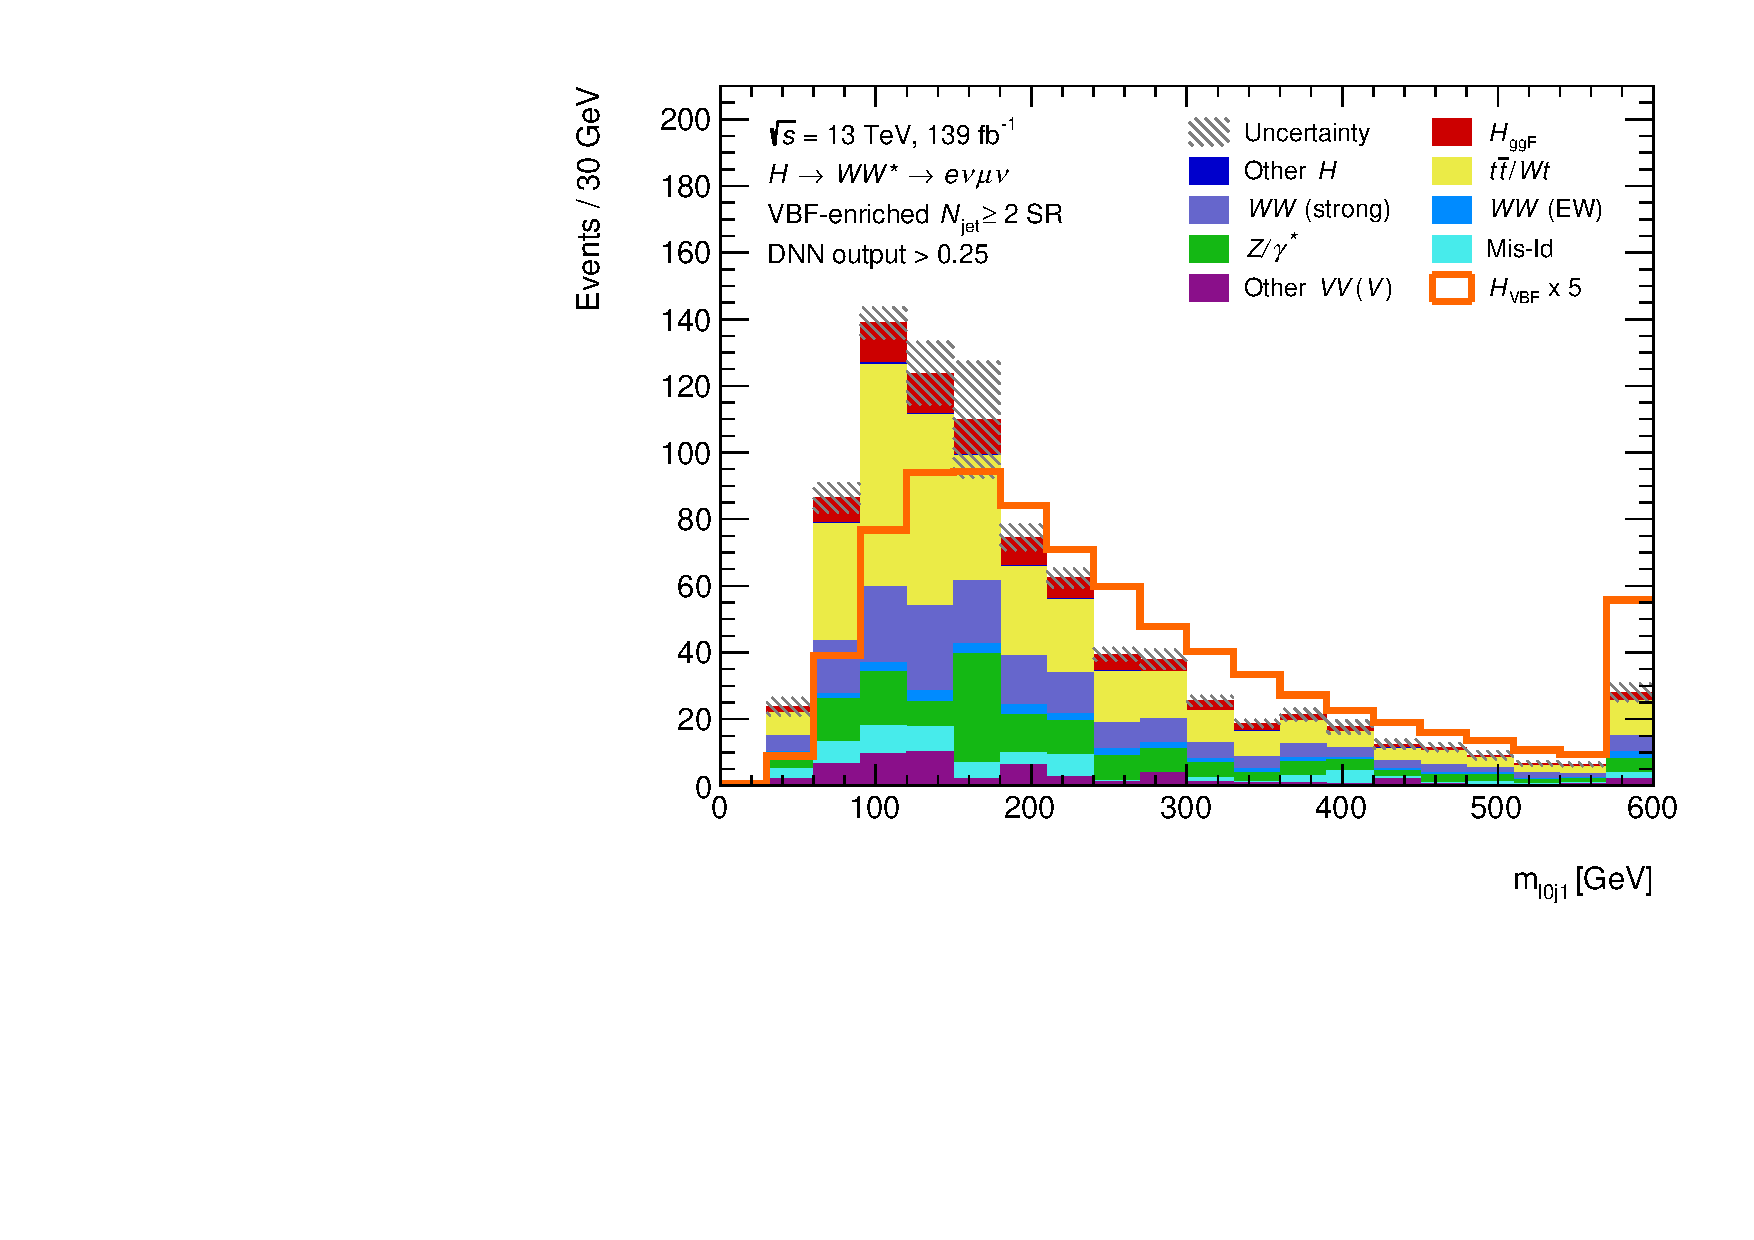
\includegraphics[width=0.32\textwidth]{figures/hww/dnn/blinded/run2-emme-CutVBFSR_DNN25-Ml0j1-lin.pdf} \hfill
        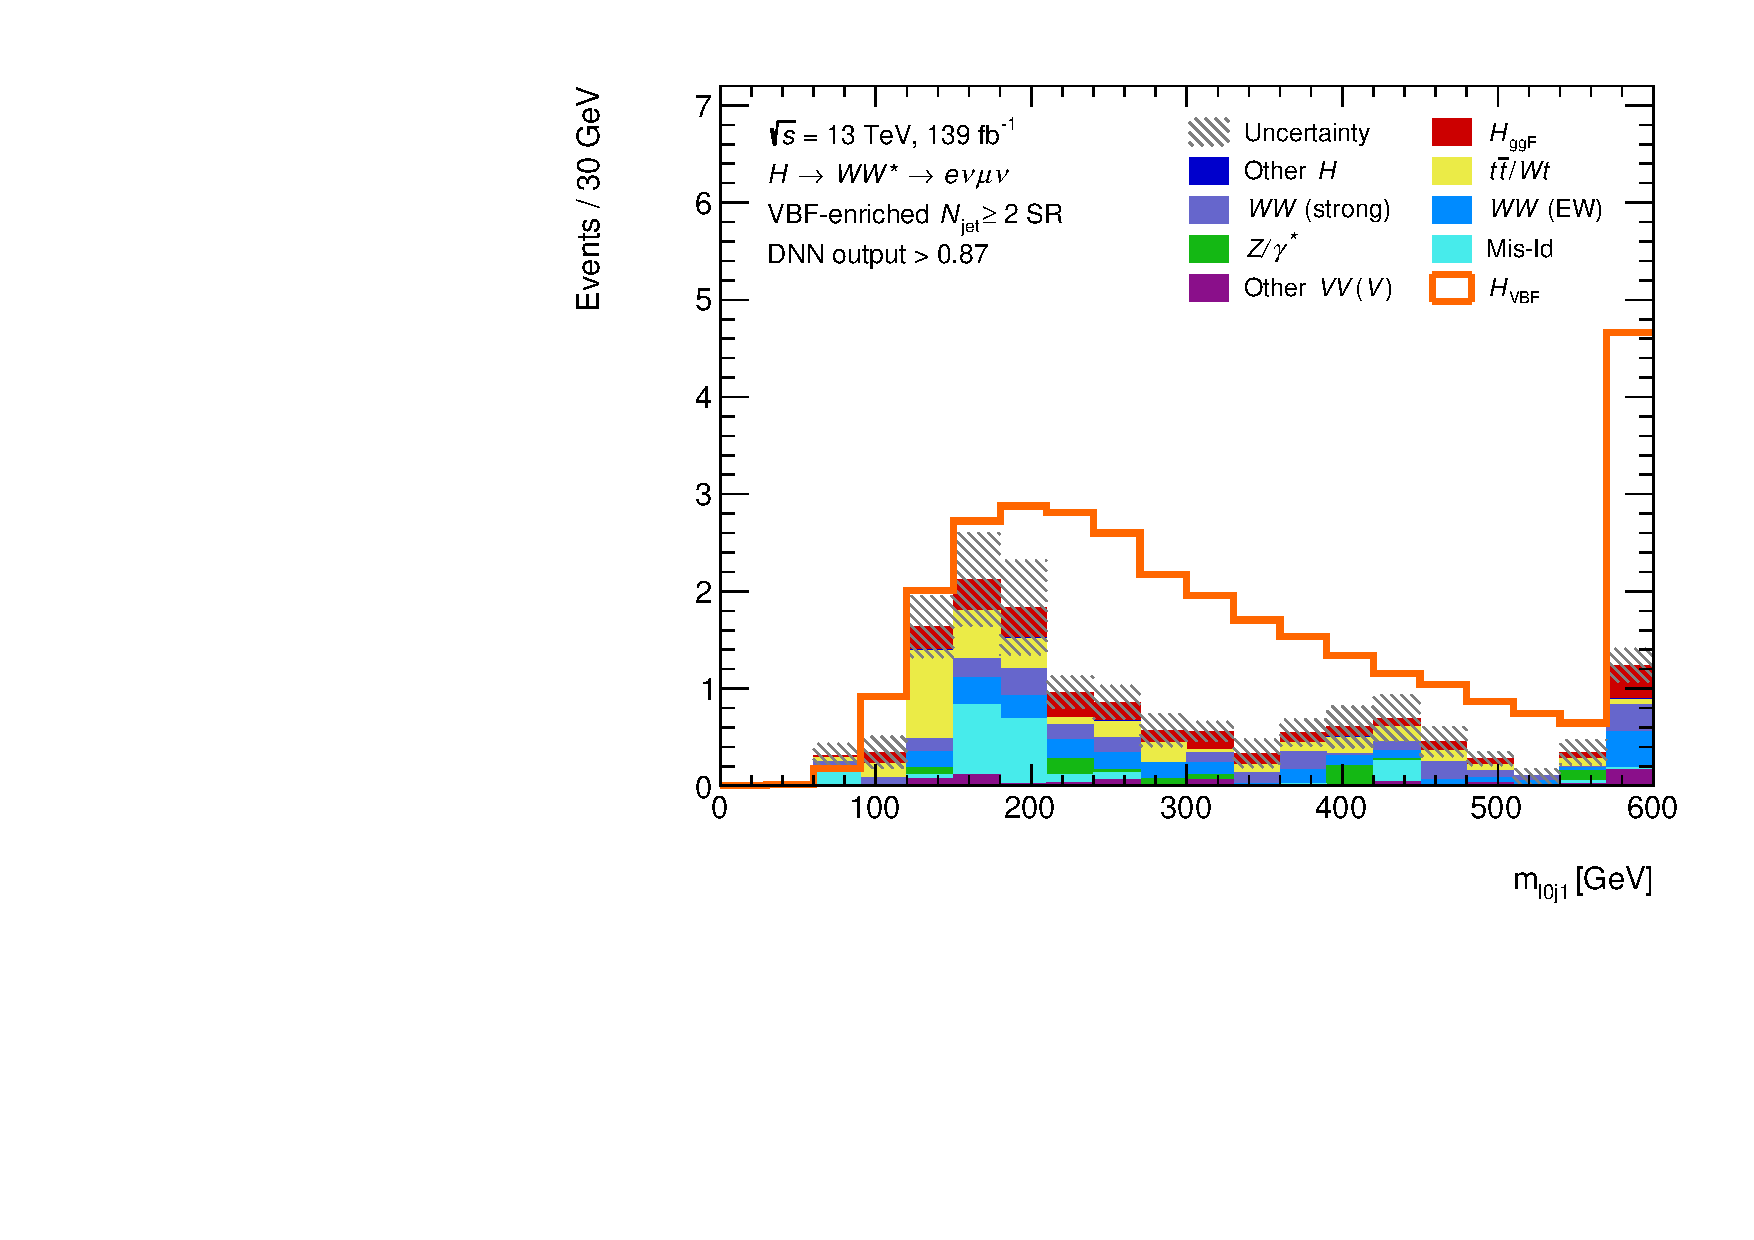
\includegraphics[width=0.32\textwidth]{figures/hww/dnn/blinded/run2-emme-CutVBFSR_DNN87-Ml0j1-lin.pdf}
    } \\
    \subfloat[$\mltwojtwo$]{
        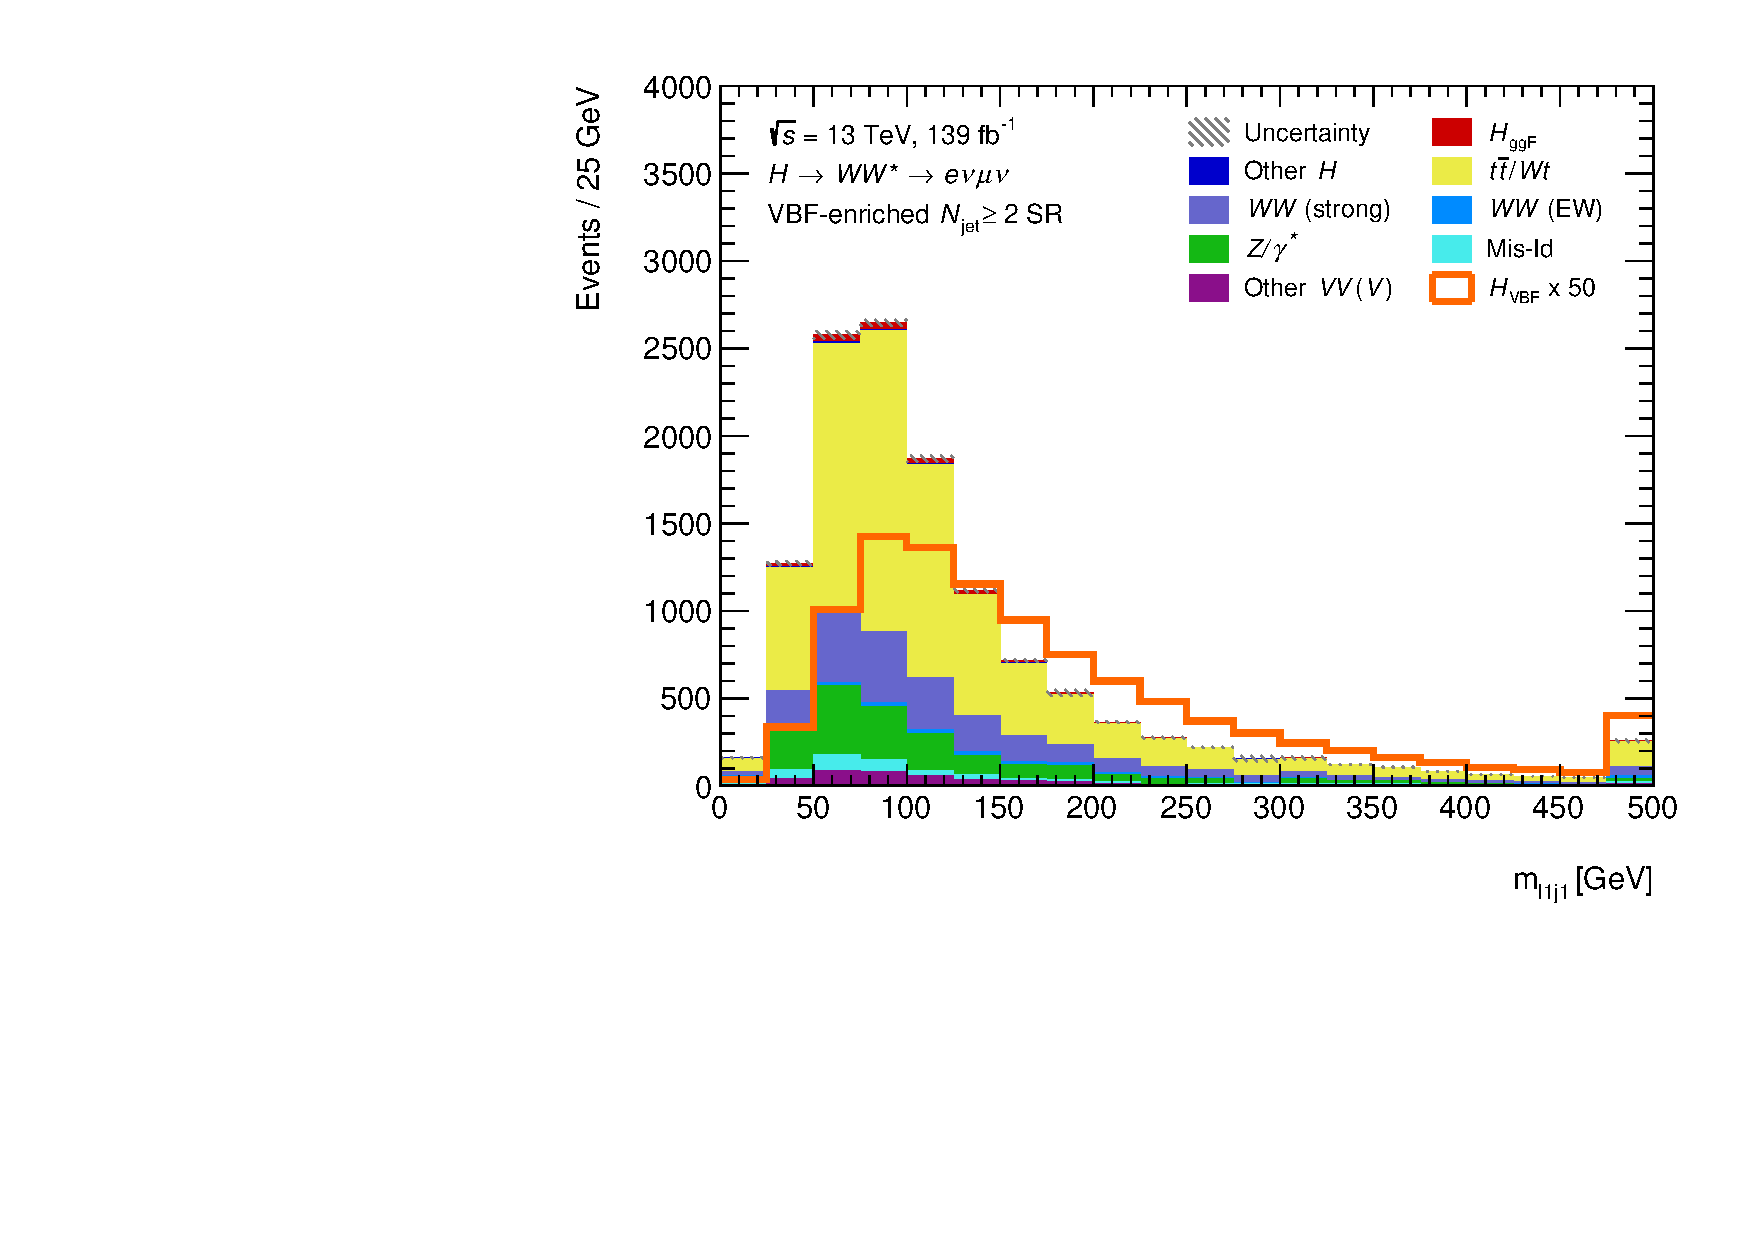
\includegraphics[width=0.32\textwidth]{figures/hww/dnn/blinded/run2-emme-CutVBF_SR-Ml1j1-lin.pdf} \hfill
        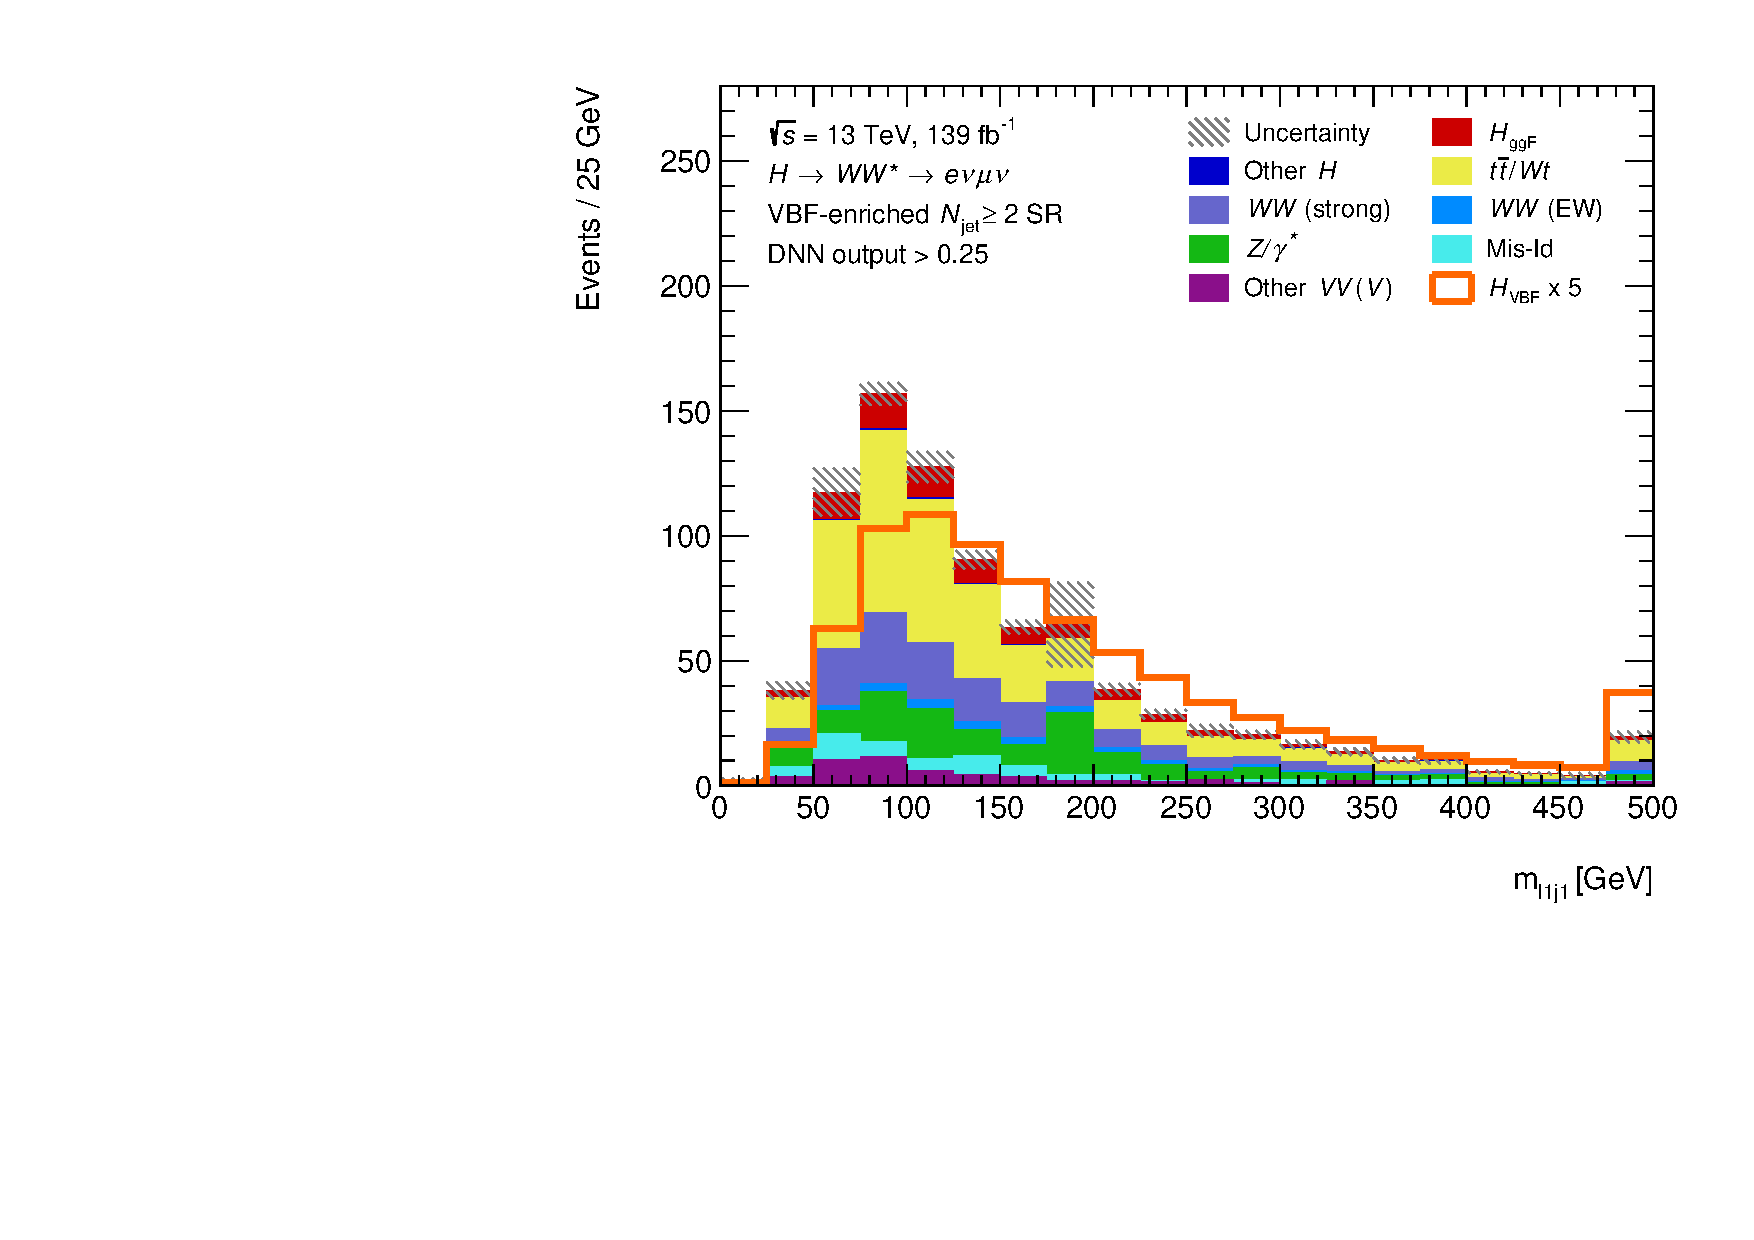
\includegraphics[width=0.32\textwidth]{figures/hww/dnn/blinded/run2-emme-CutVBFSR_DNN25-Ml1j1-lin.pdf} \hfill
        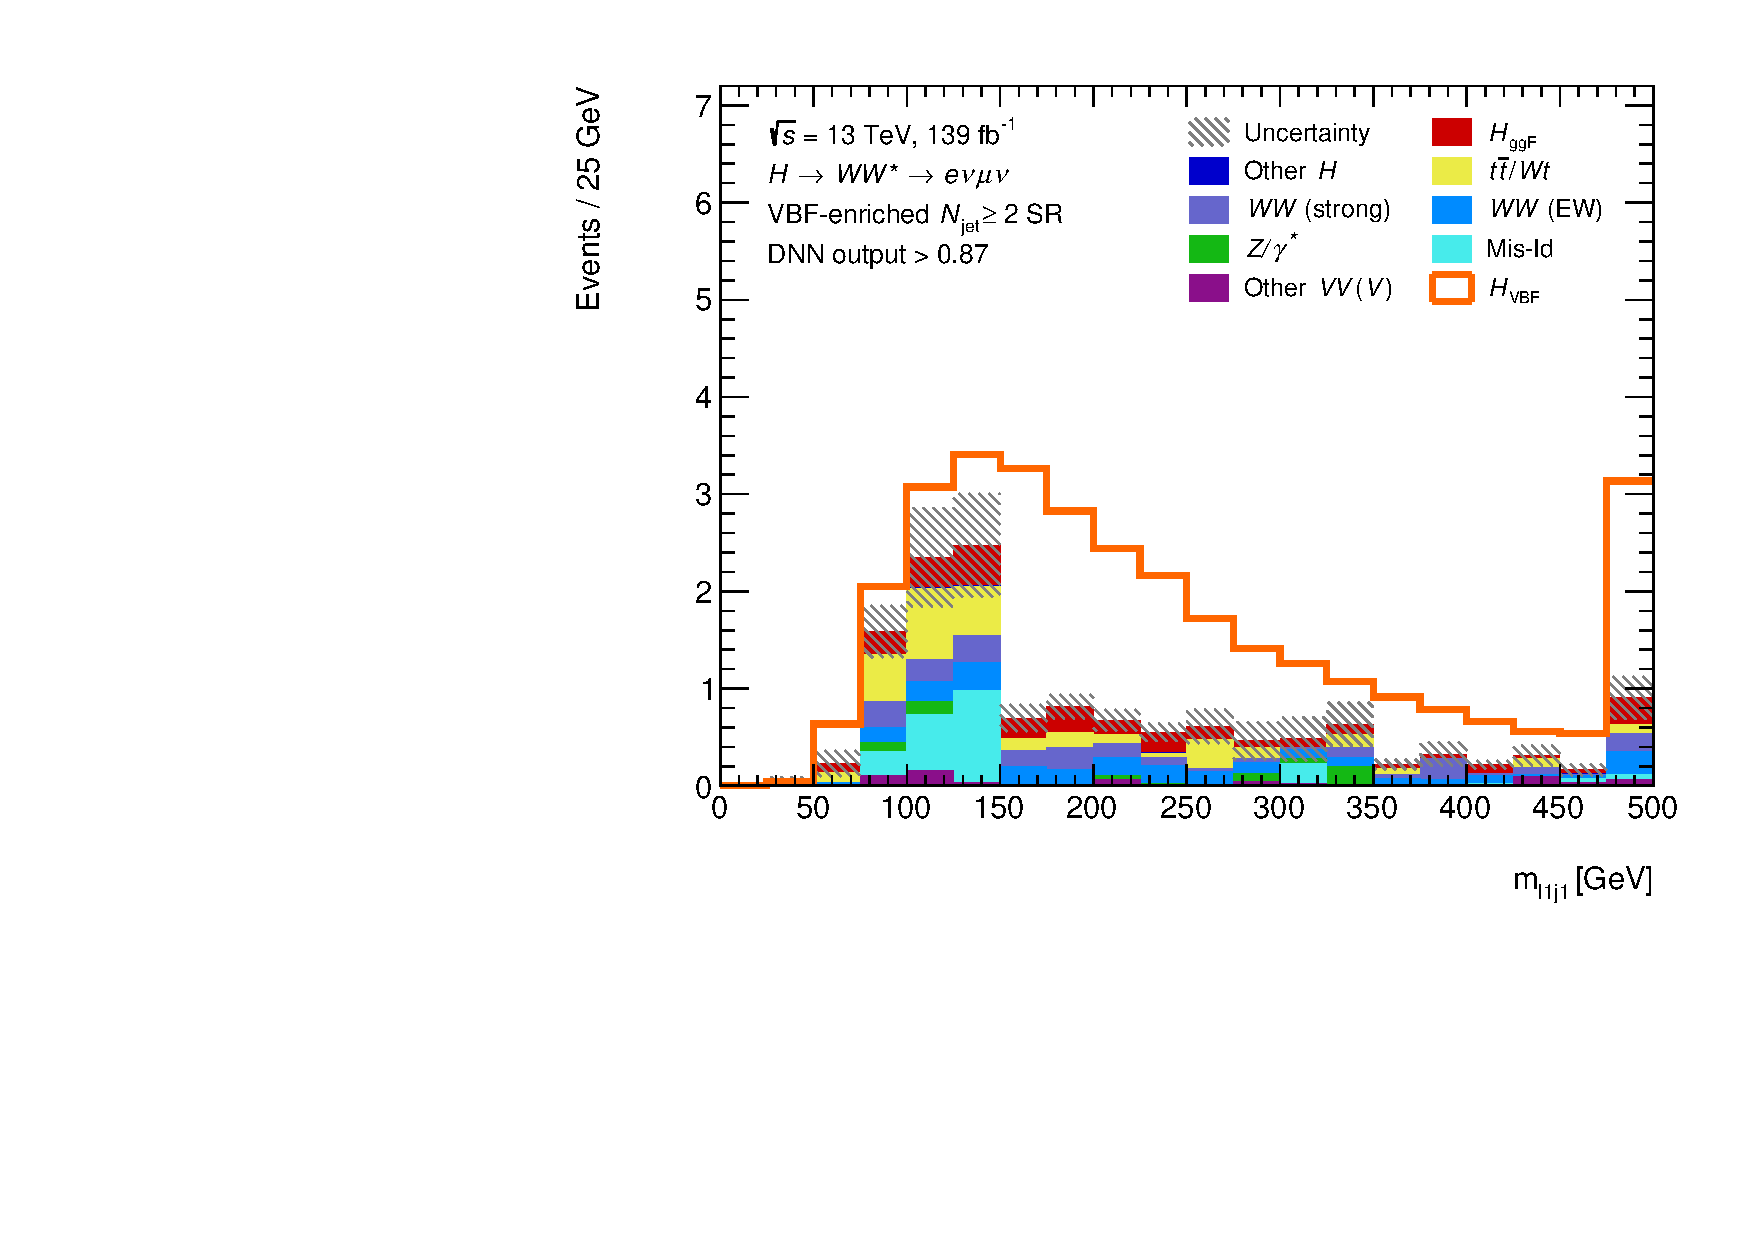
\includegraphics[width=0.32\textwidth]{figures/hww/dnn/blinded/run2-emme-CutVBFSR_DNN87-Ml1j1-lin.pdf}
    } 
    {\caption{Distributions of $\mlonejone$, $\mltwojone$, $\mlonejtwo$, and $\mltwojtwo$ in the VBF signal region.
            Each row shows one variable with different cuts on the DNN output distribution being applied in different columns.
            \label{app:fig:dnn-inputs-vbf-top2} }}
\end{figure}


\begin{figure}[h]
    \centering
    \subfloat[$\pTjone$]{
        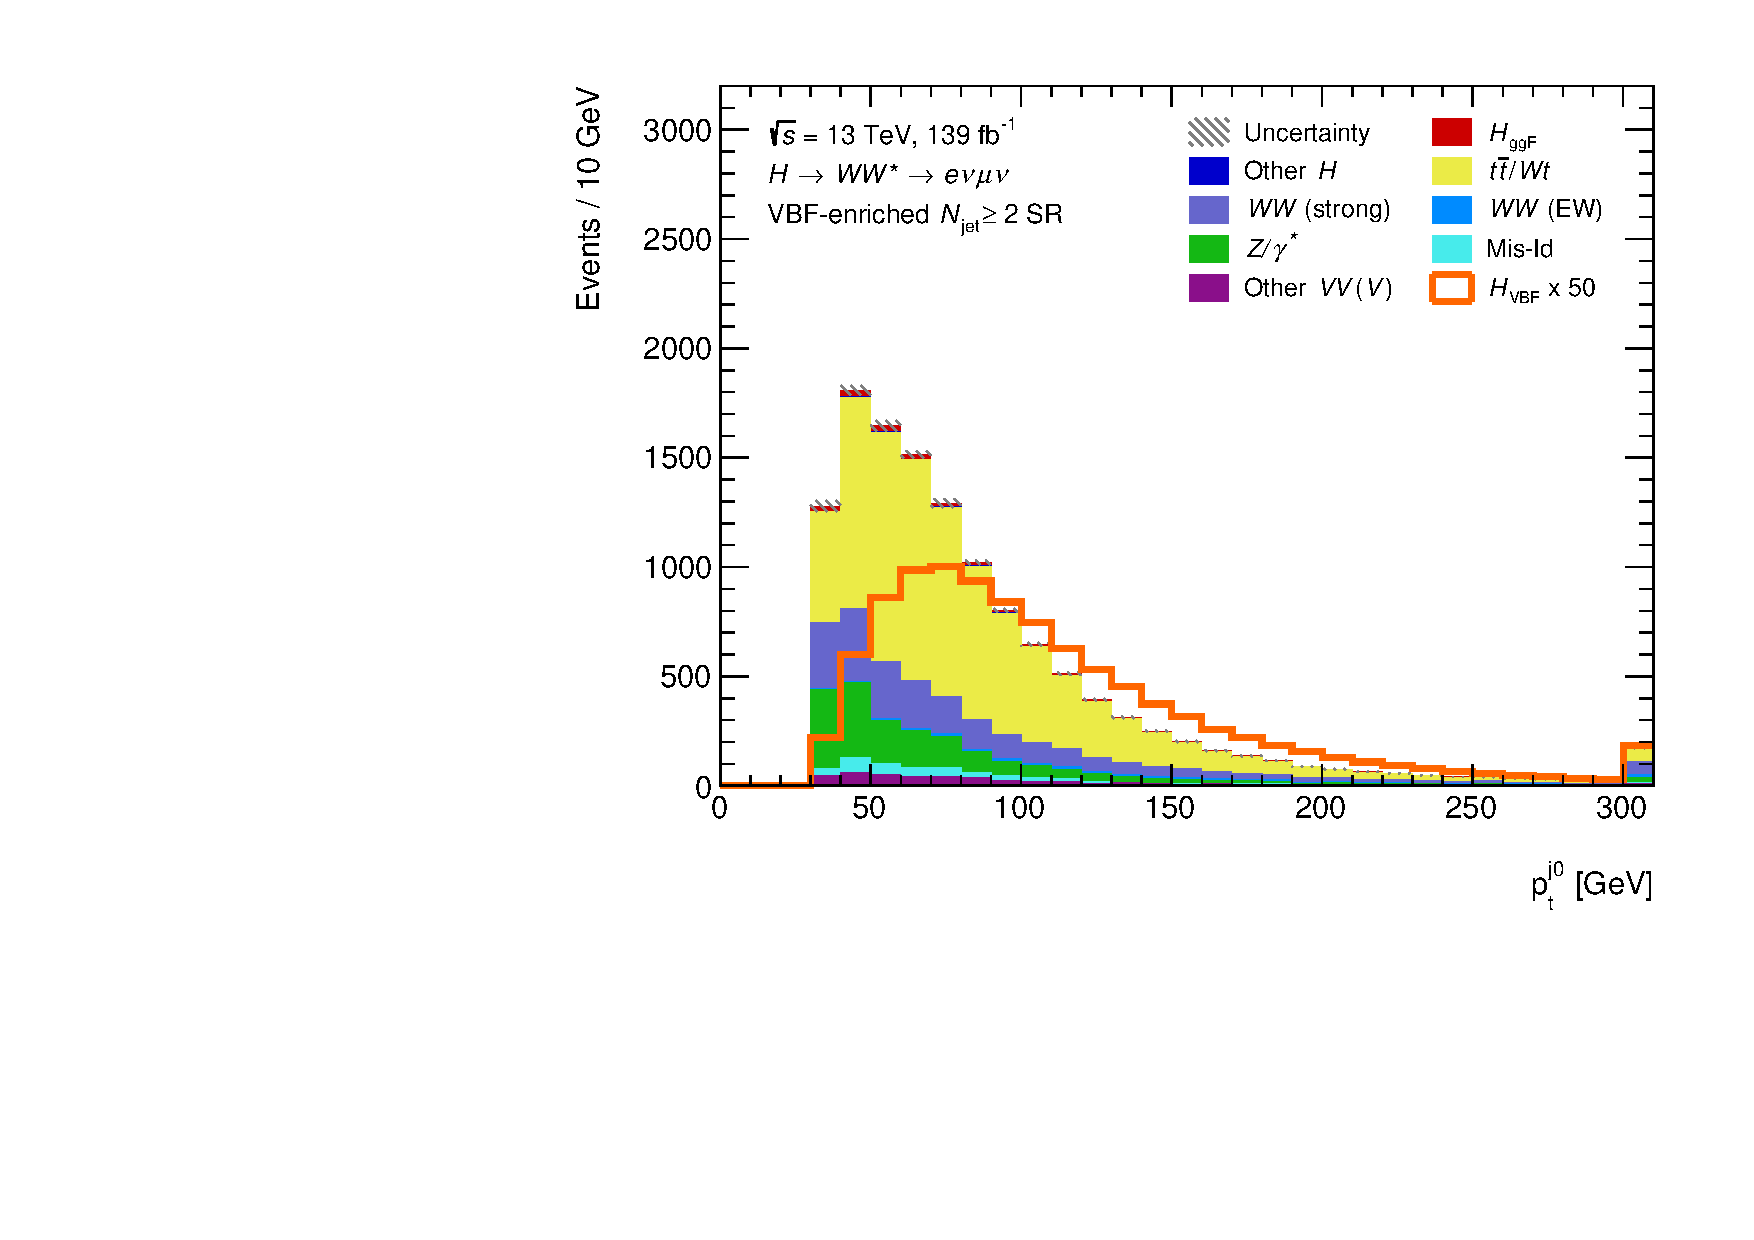
\includegraphics[width=0.32\textwidth]{figures/hww/dnn/blinded/run2-emme-CutVBF_SR-leadJetPt-lin.pdf} \hfill
        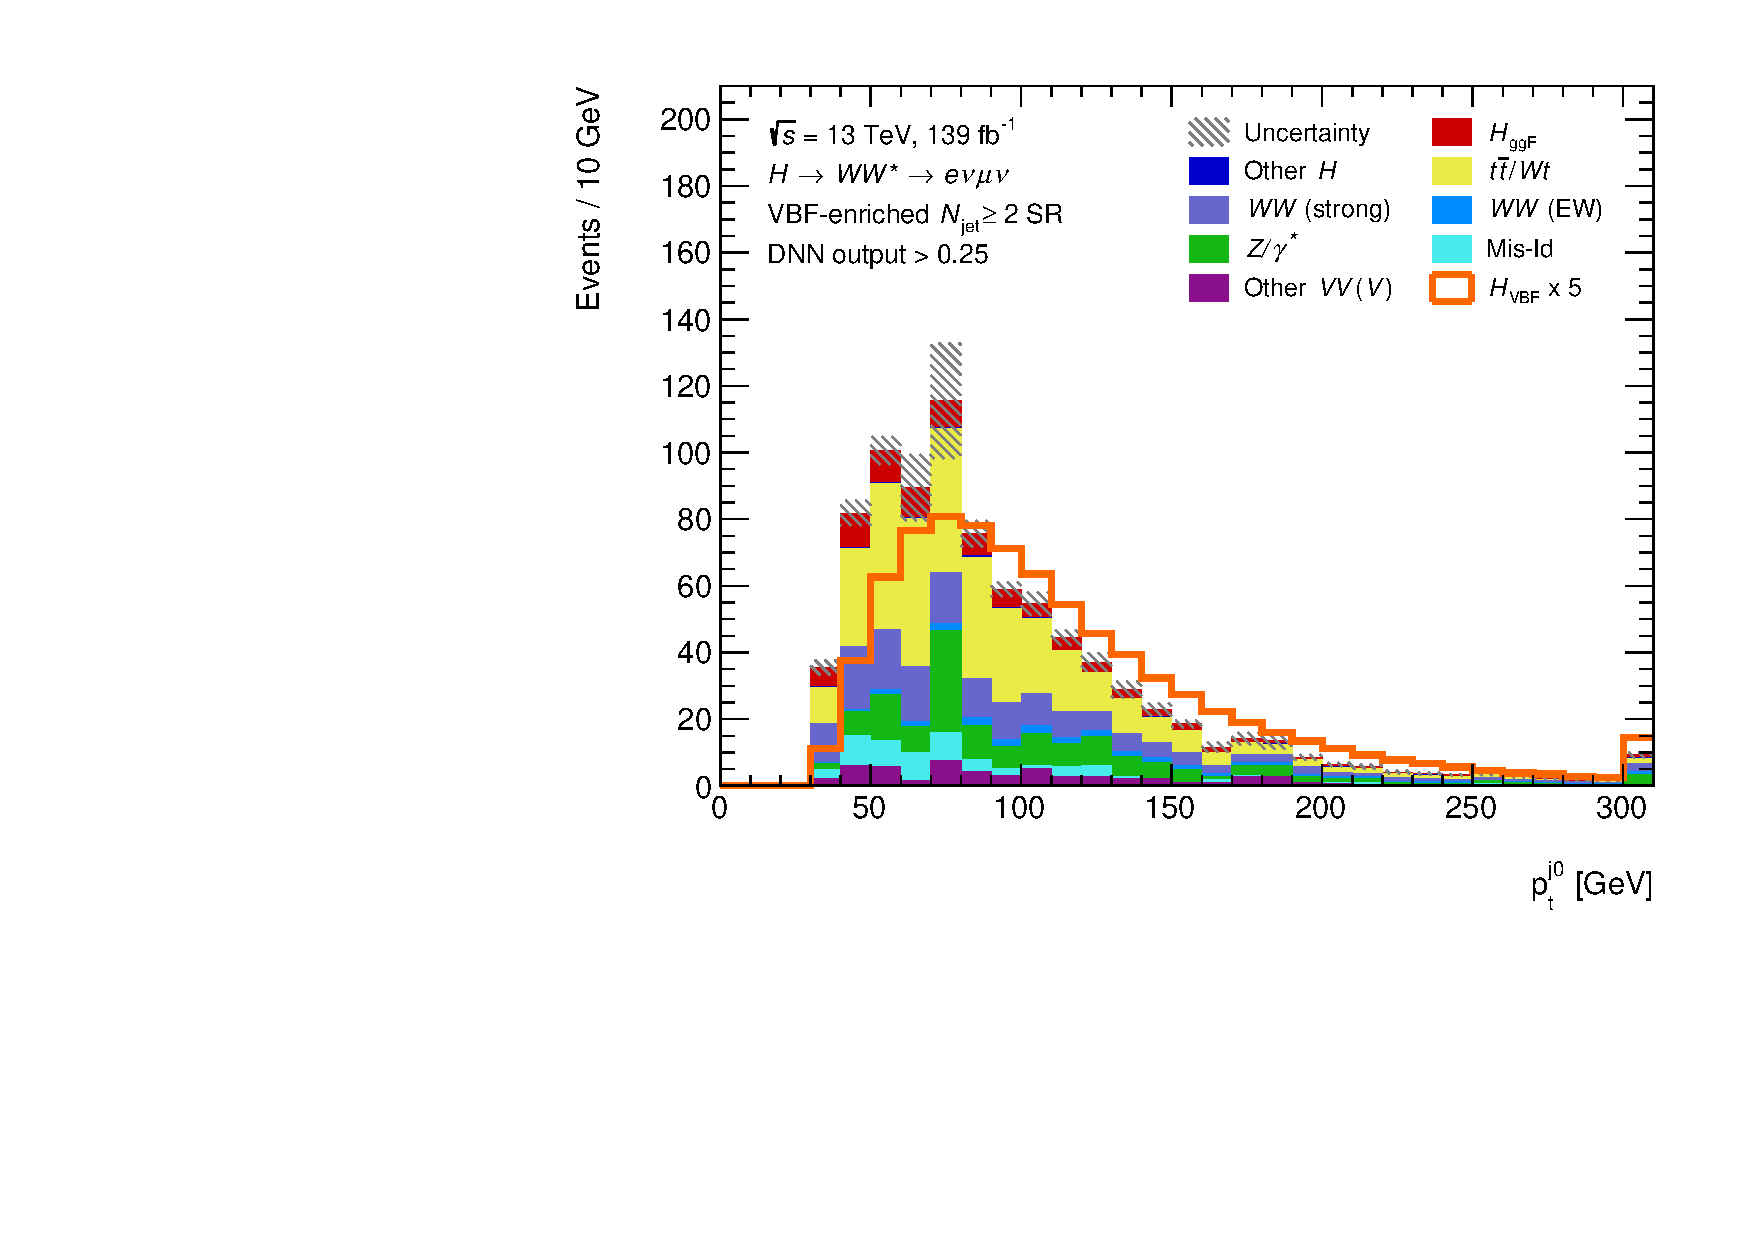
\includegraphics[width=0.32\textwidth]{figures/hww/dnn/blinded/run2-emme-CutVBFSR_DNN25-leadJetPt-lin.pdf} \hfill
        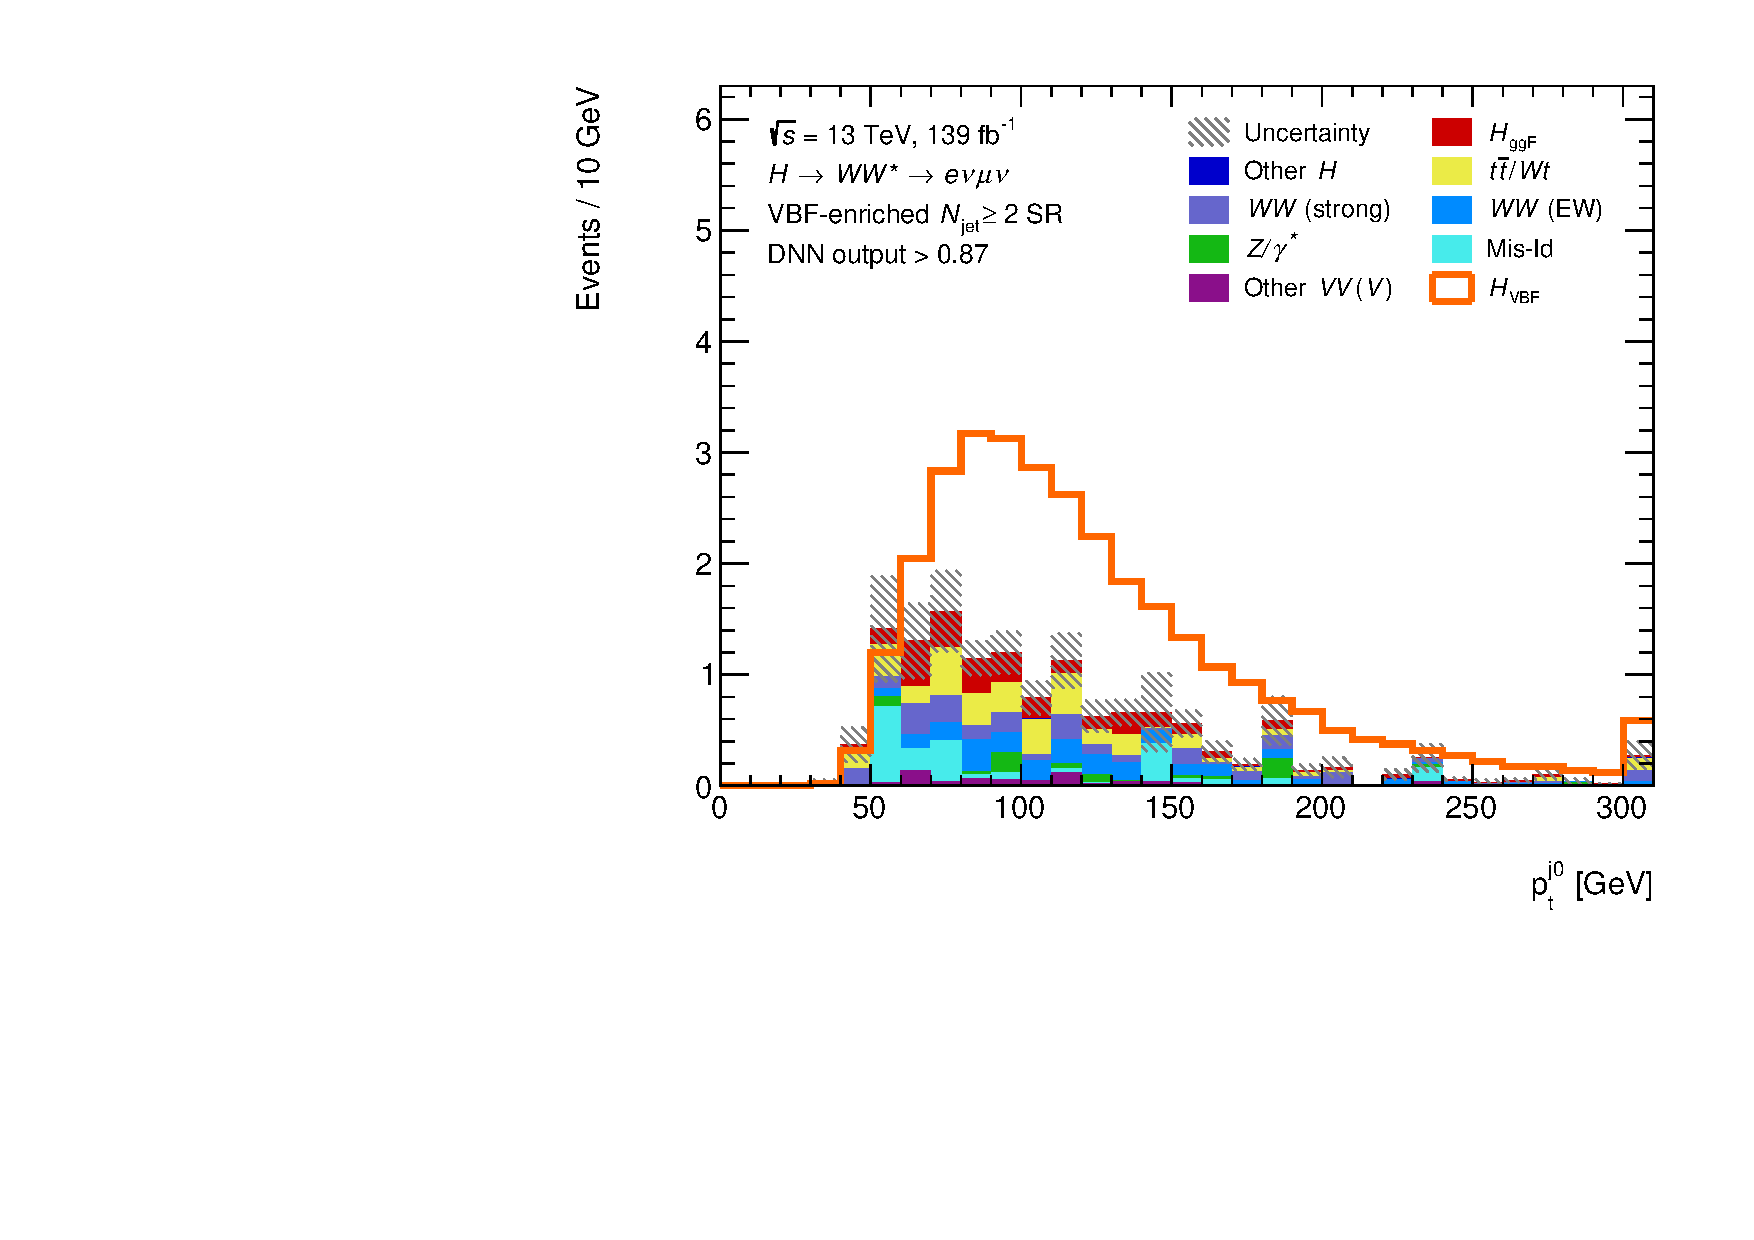
\includegraphics[width=0.32\textwidth]{figures/hww/dnn/blinded/run2-emme-CutVBFSR_DNN87-leadJetPt-lin.pdf}
    } \\
    \subfloat[$\pTjtwo$]{
        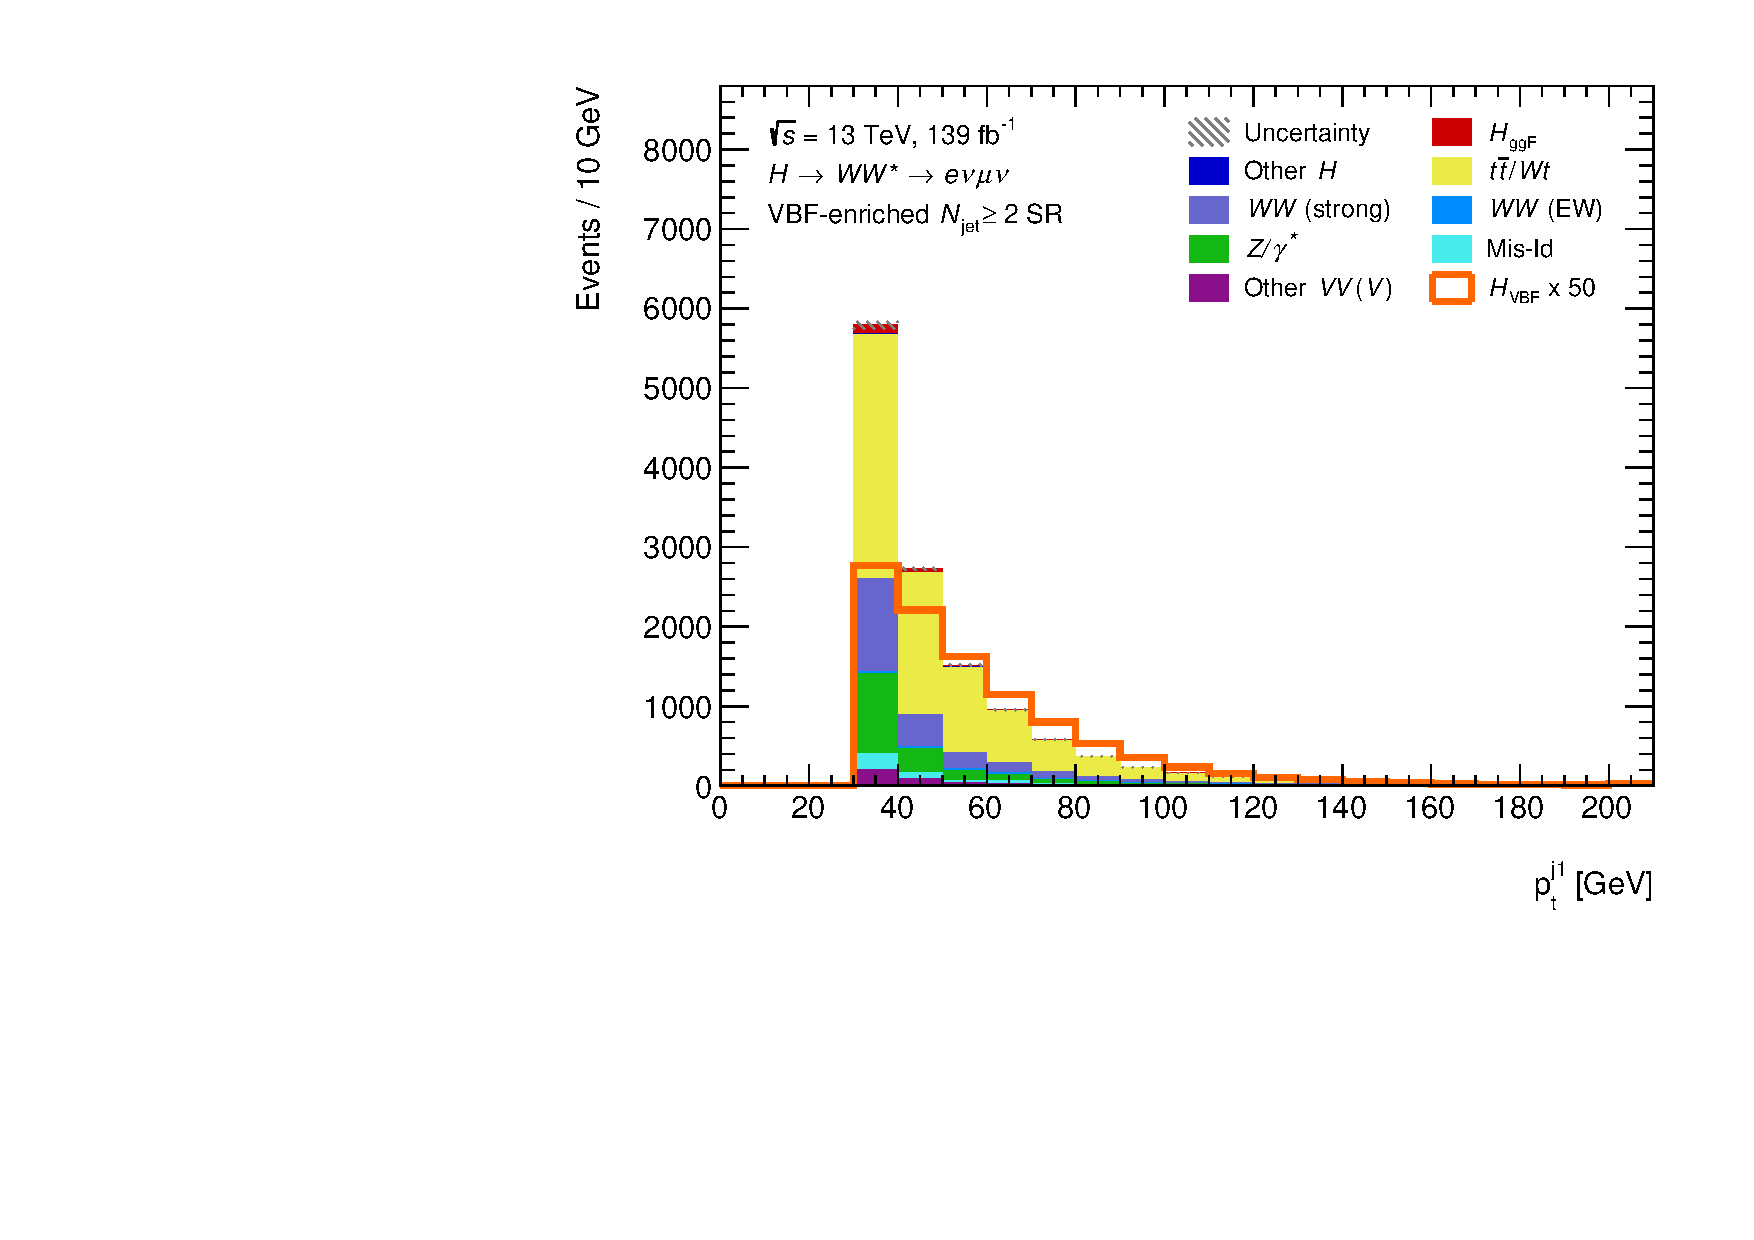
\includegraphics[width=0.32\textwidth]{figures/hww/dnn/blinded/run2-emme-CutVBF_SR-subleadJetPt-lin.pdf} \hfill
        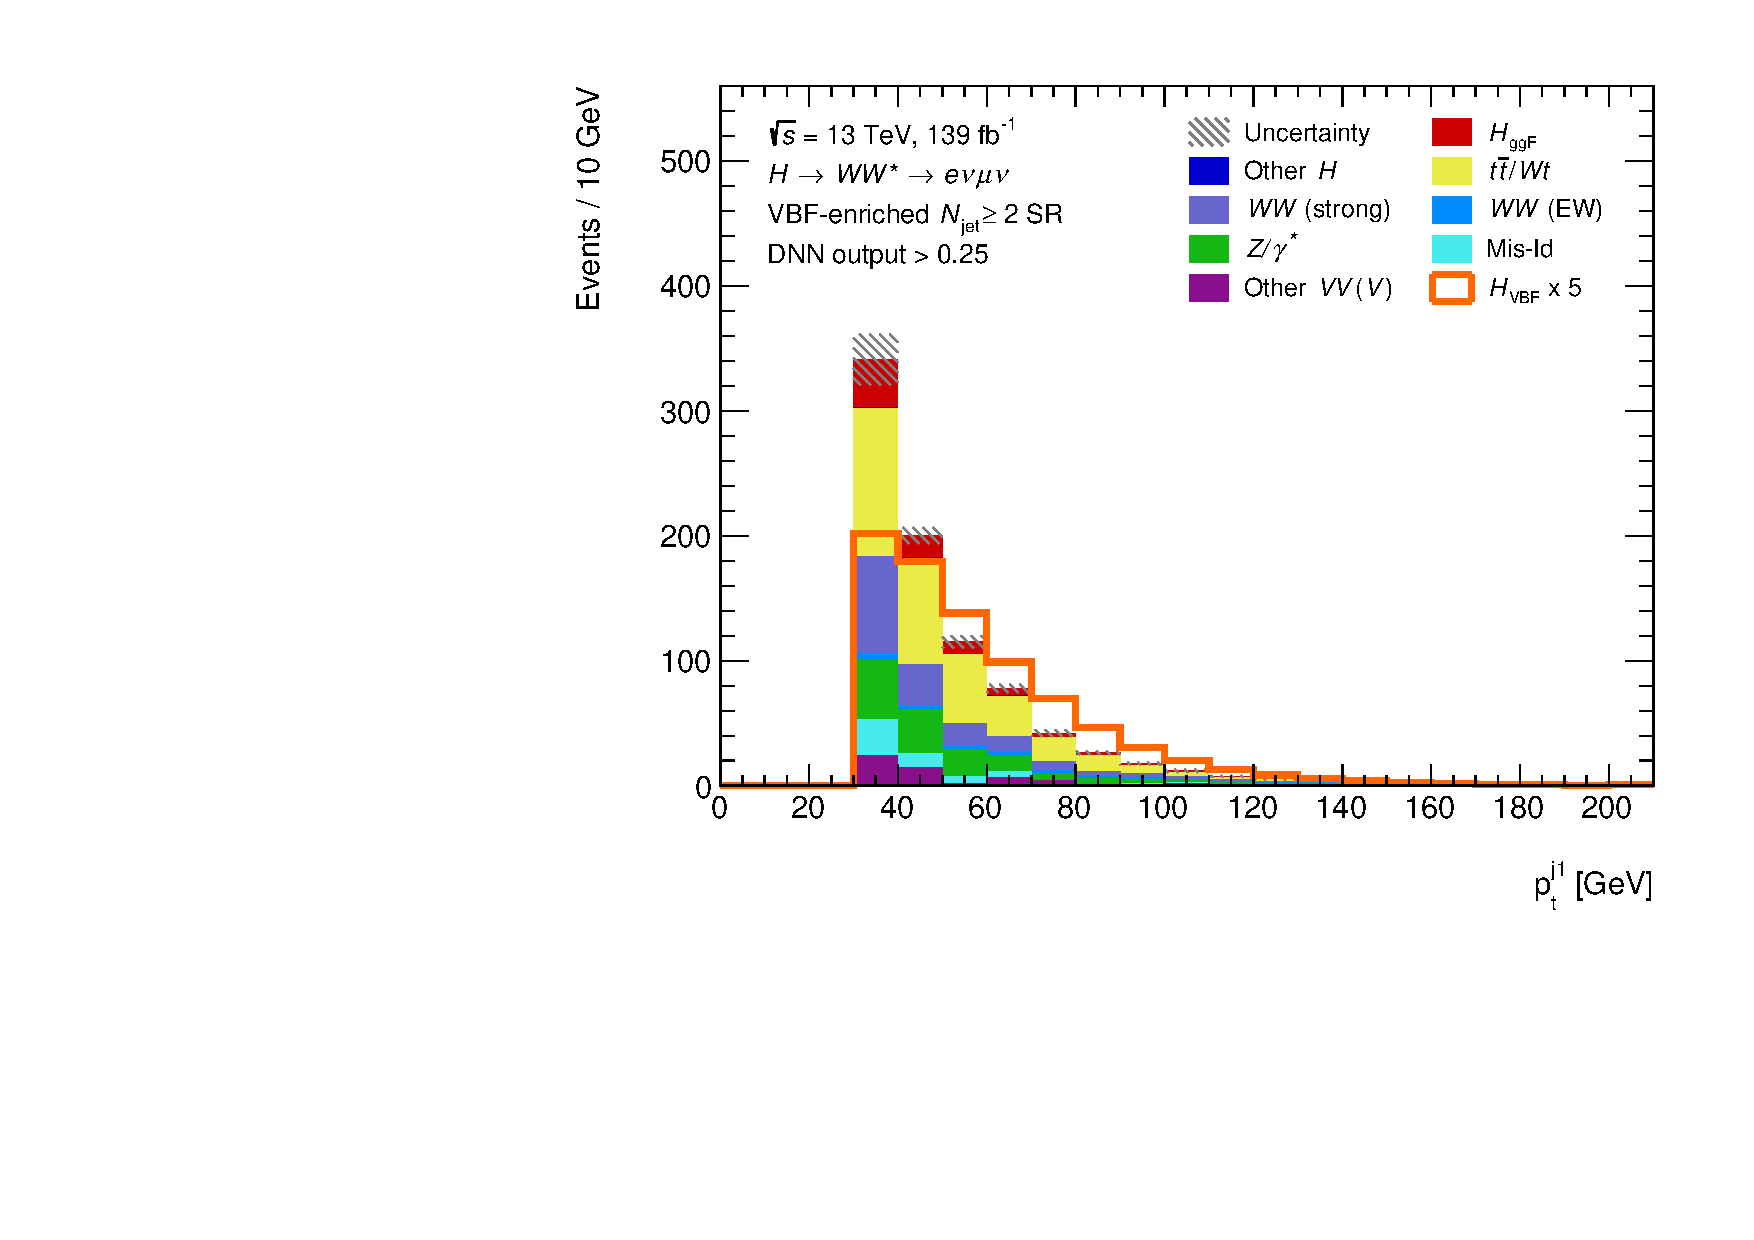
\includegraphics[width=0.32\textwidth]{figures/hww/dnn/blinded/run2-emme-CutVBFSR_DNN25-subleadJetPt-lin.pdf} \hfill
        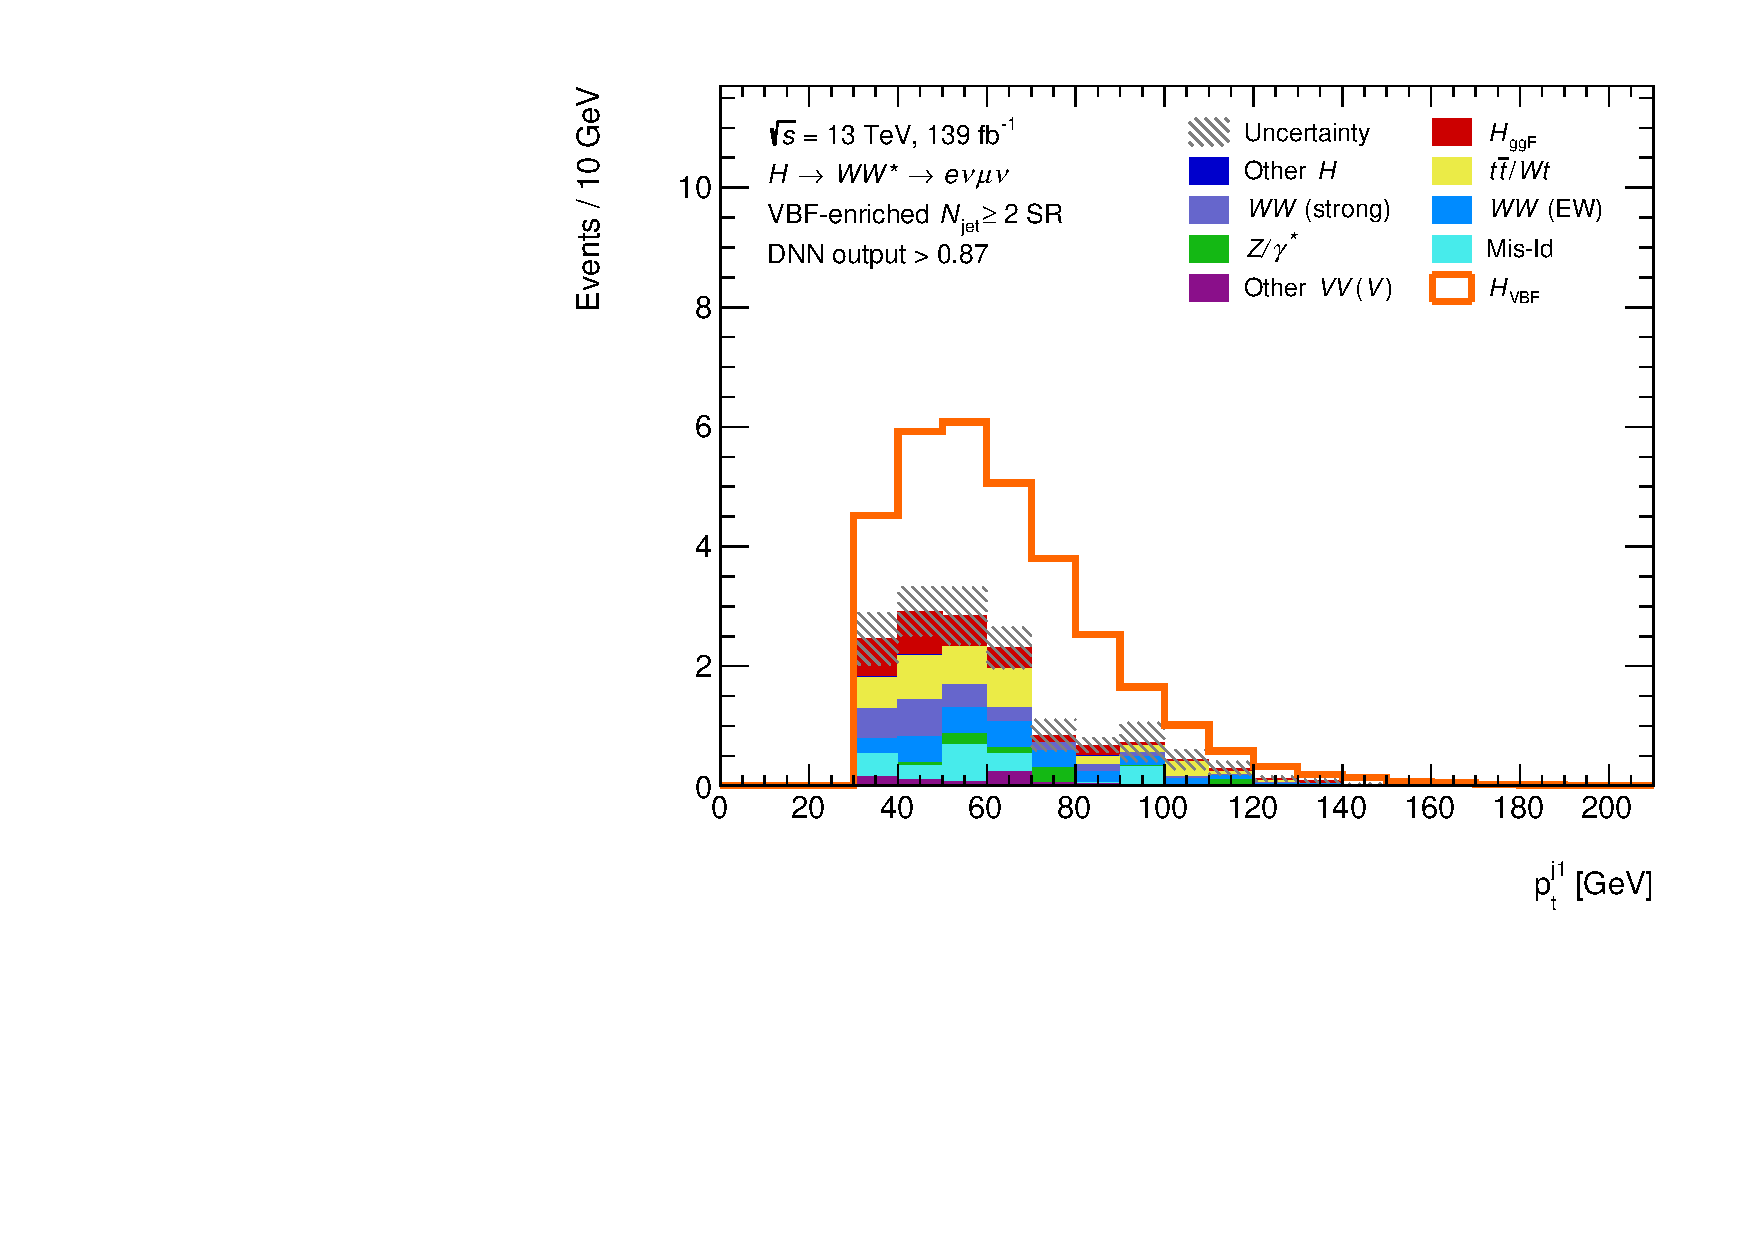
\includegraphics[width=0.32\textwidth]{figures/hww/dnn/blinded/run2-emme-CutVBFSR_DNN87-subleadJetPt-lin.pdf}
    } \\
    \subfloat[$\pTjthree$]{
        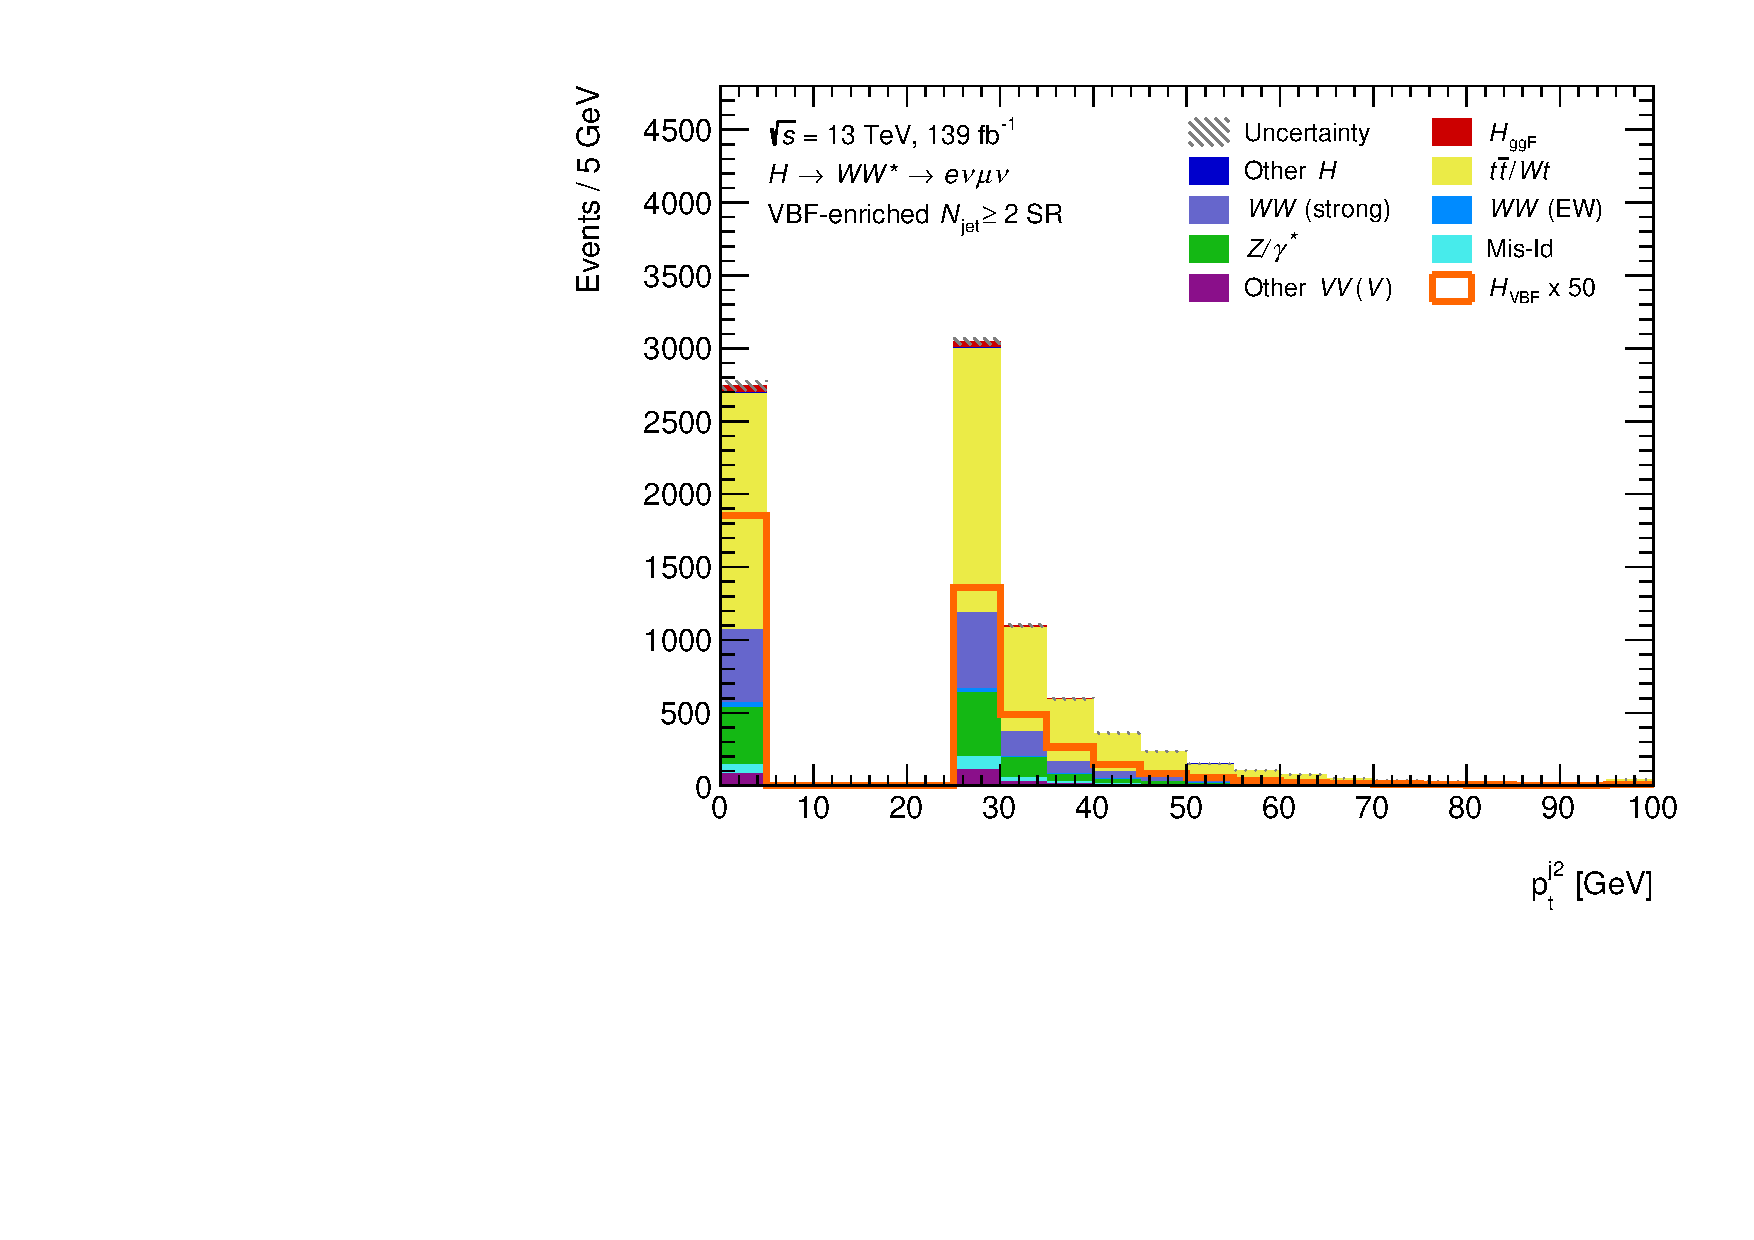
\includegraphics[width=0.32\textwidth]{figures/hww/dnn/blinded/run2-emme-CutVBF_SR-thirdJetPt-lin.pdf} \hfill
        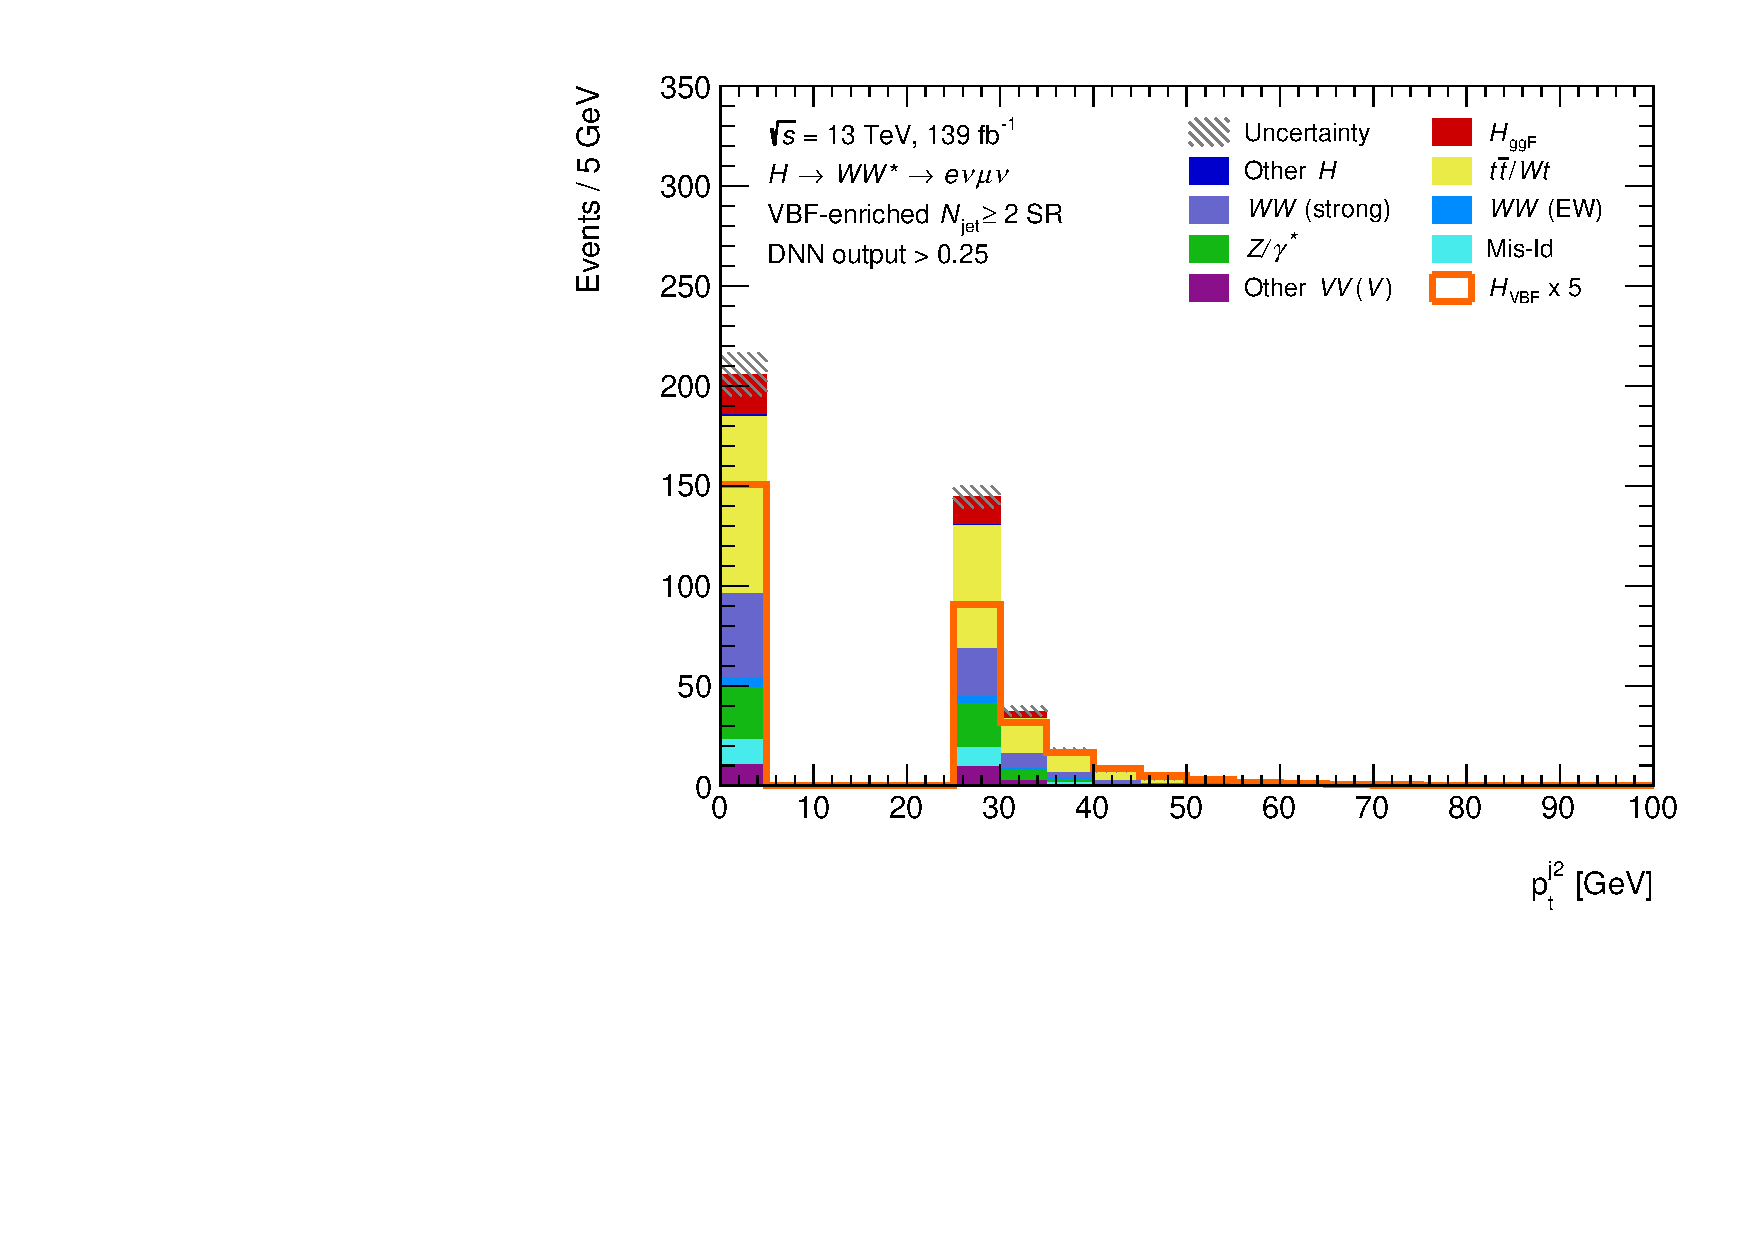
\includegraphics[width=0.32\textwidth]{figures/hww/dnn/blinded/run2-emme-CutVBFSR_DNN25-thirdJetPt-lin.pdf} \hfill
        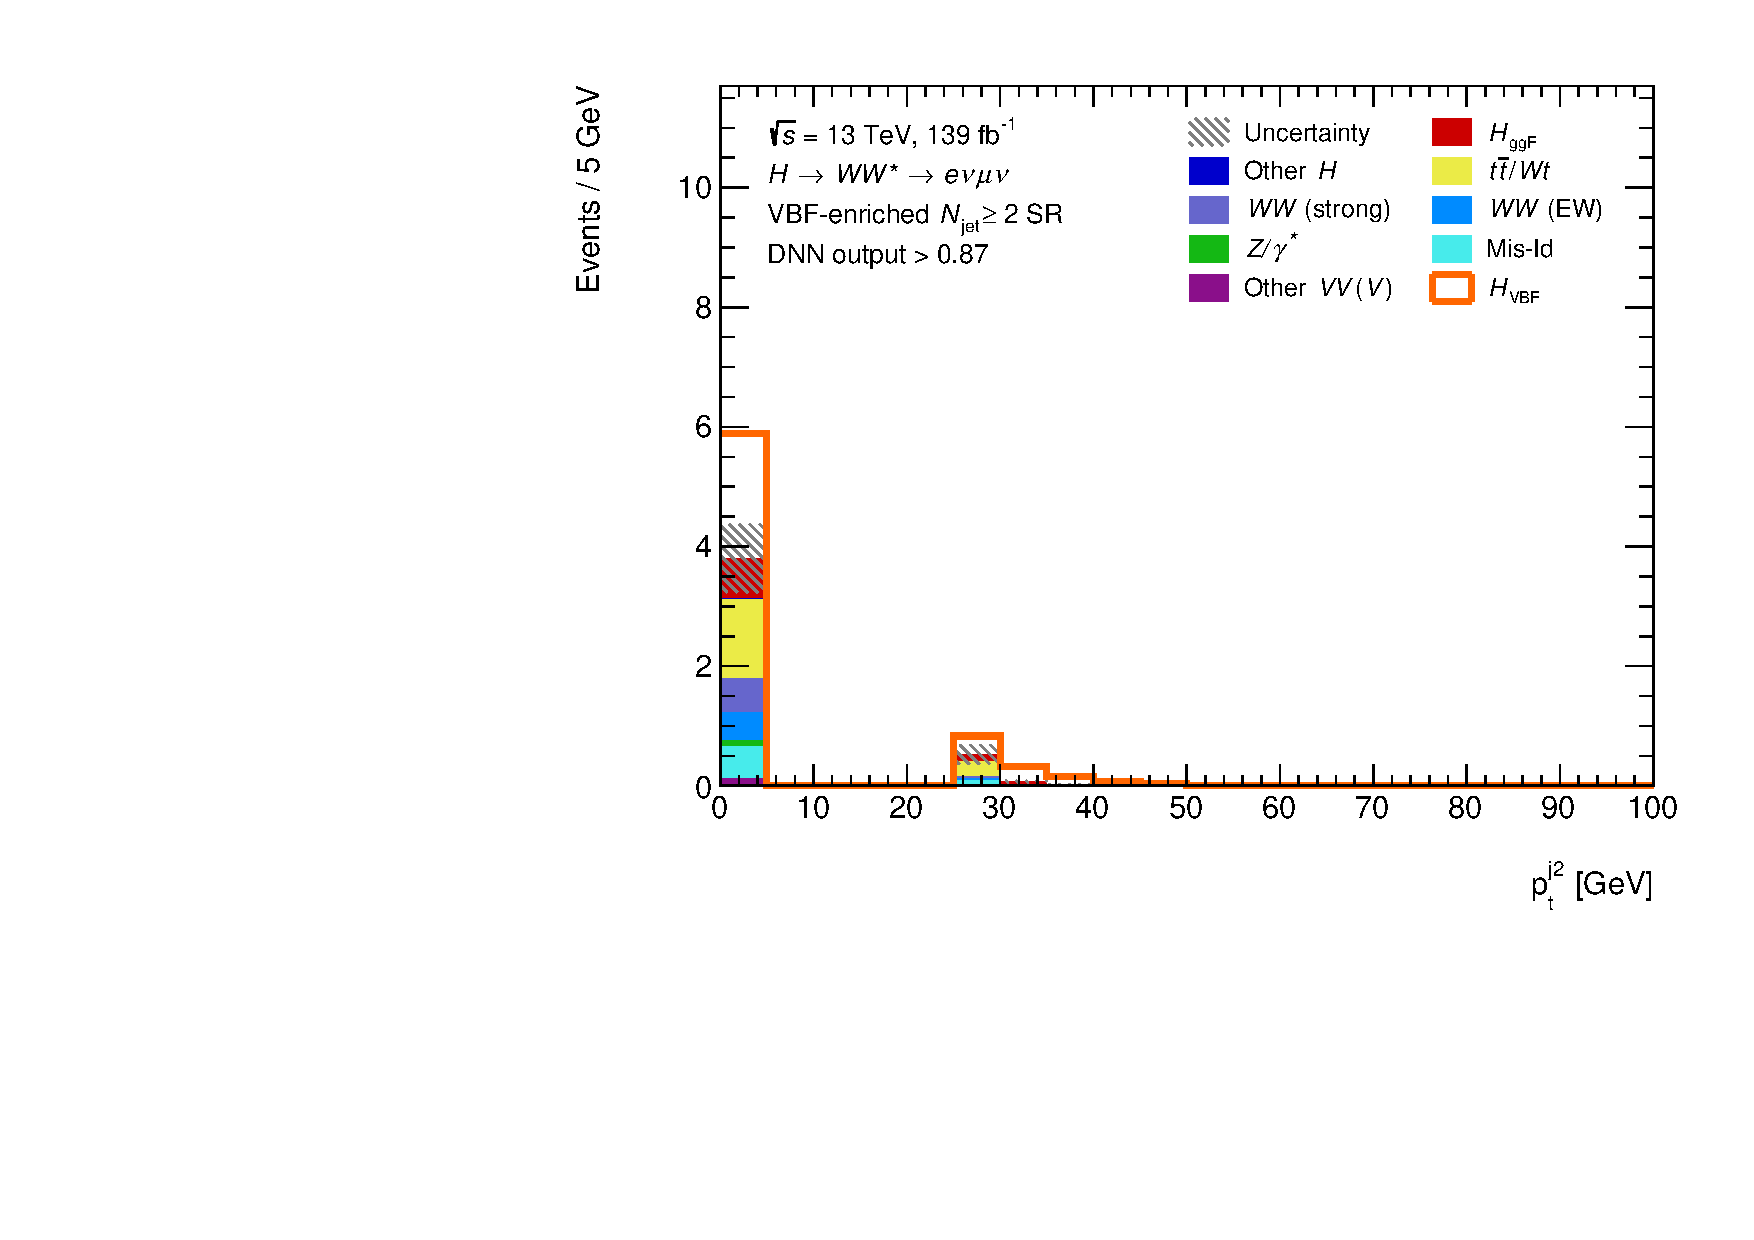
\includegraphics[width=0.32\textwidth]{figures/hww/dnn/blinded/run2-emme-CutVBFSR_DNN87-thirdJetPt-lin.pdf}
    } 
    {\caption{Distributions of $\pTjone$, $\pTjtwo$, and $\pTjthree$ in the VBF signal region.
            Each row shows one variable with different cuts on the DNN output distribution being applied in different columns.
            \label{app:fig:dnn-inputs-vbf-top2} }}
\end{figure}


\begin{figure}[h]
    \centering
    \subfloat[$\dphill$]{
        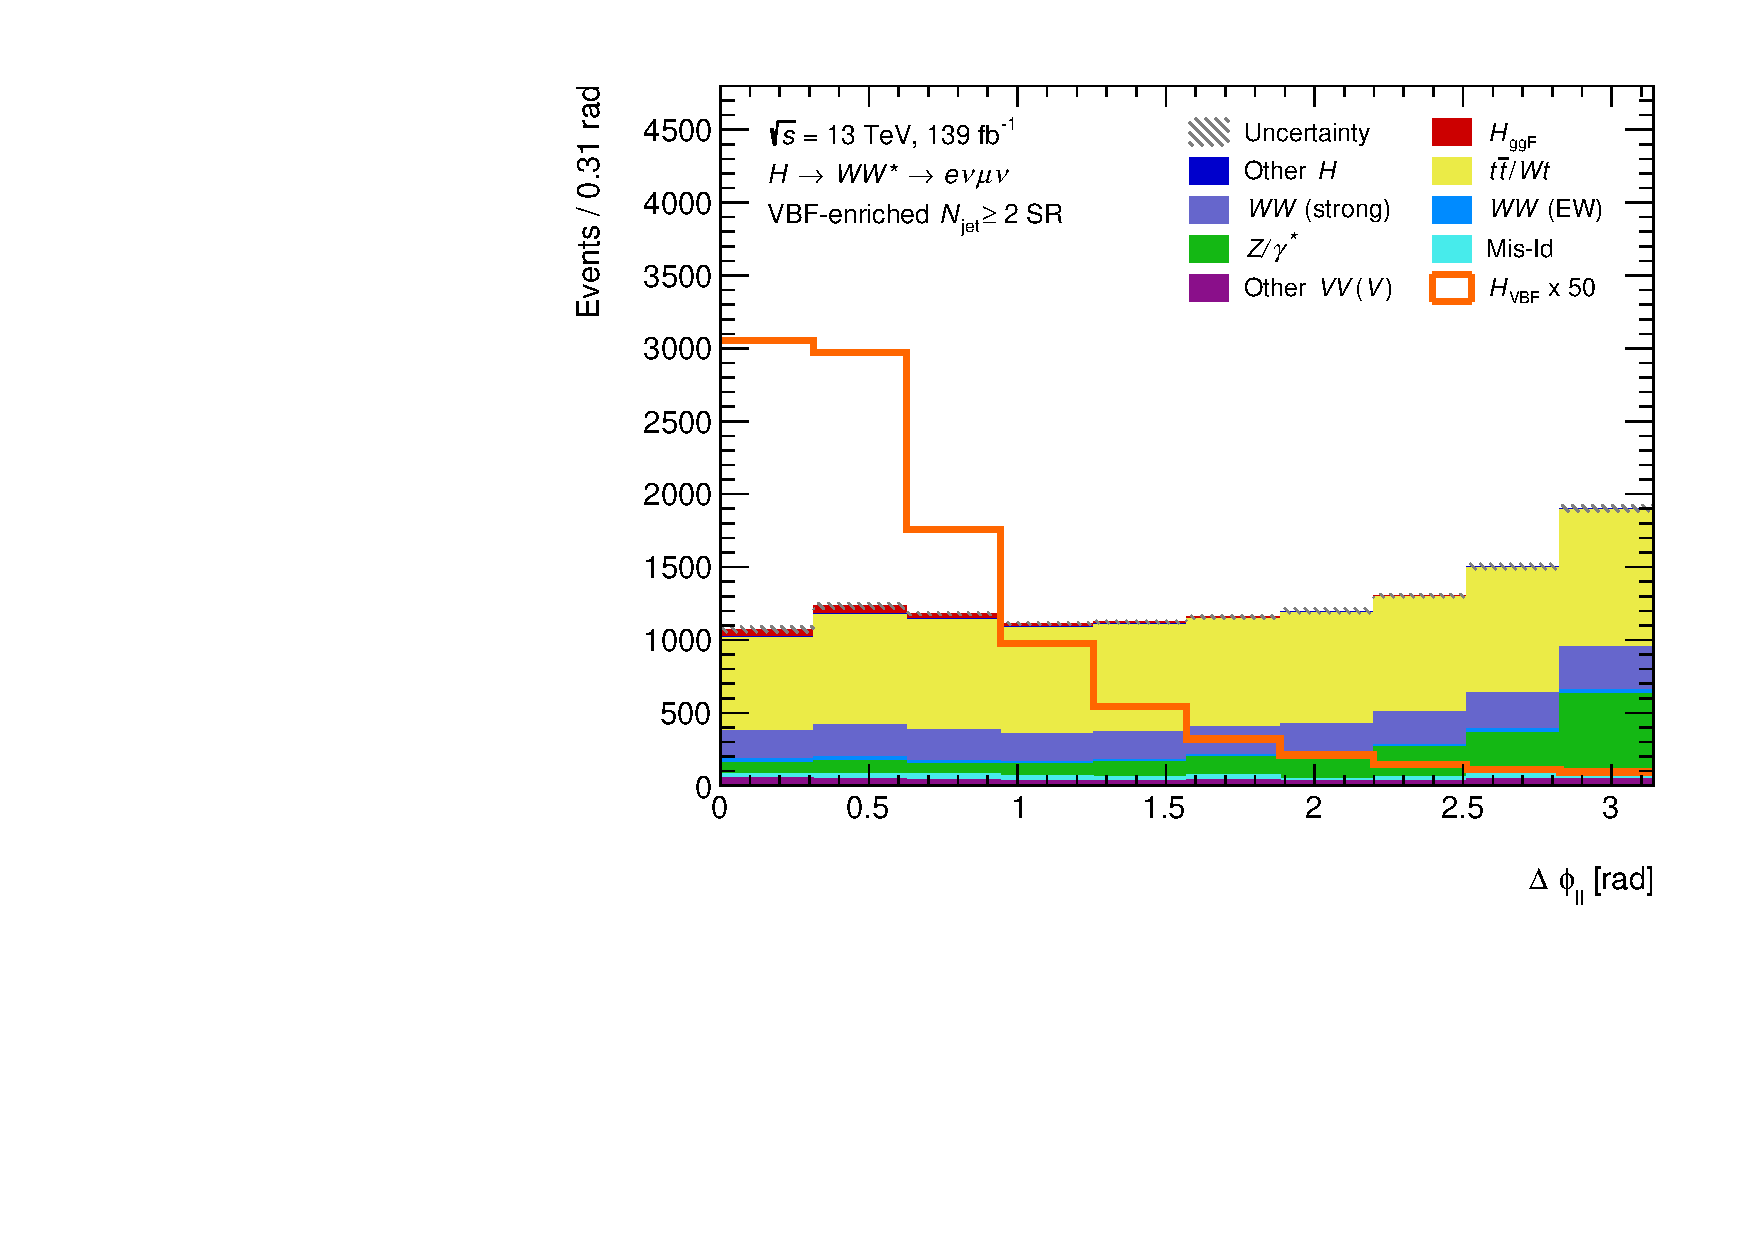
\includegraphics[width=0.32\textwidth]{figures/hww/dnn/blinded/run2-emme-CutVBF_SR-DPhill-lin.pdf} \hfill
        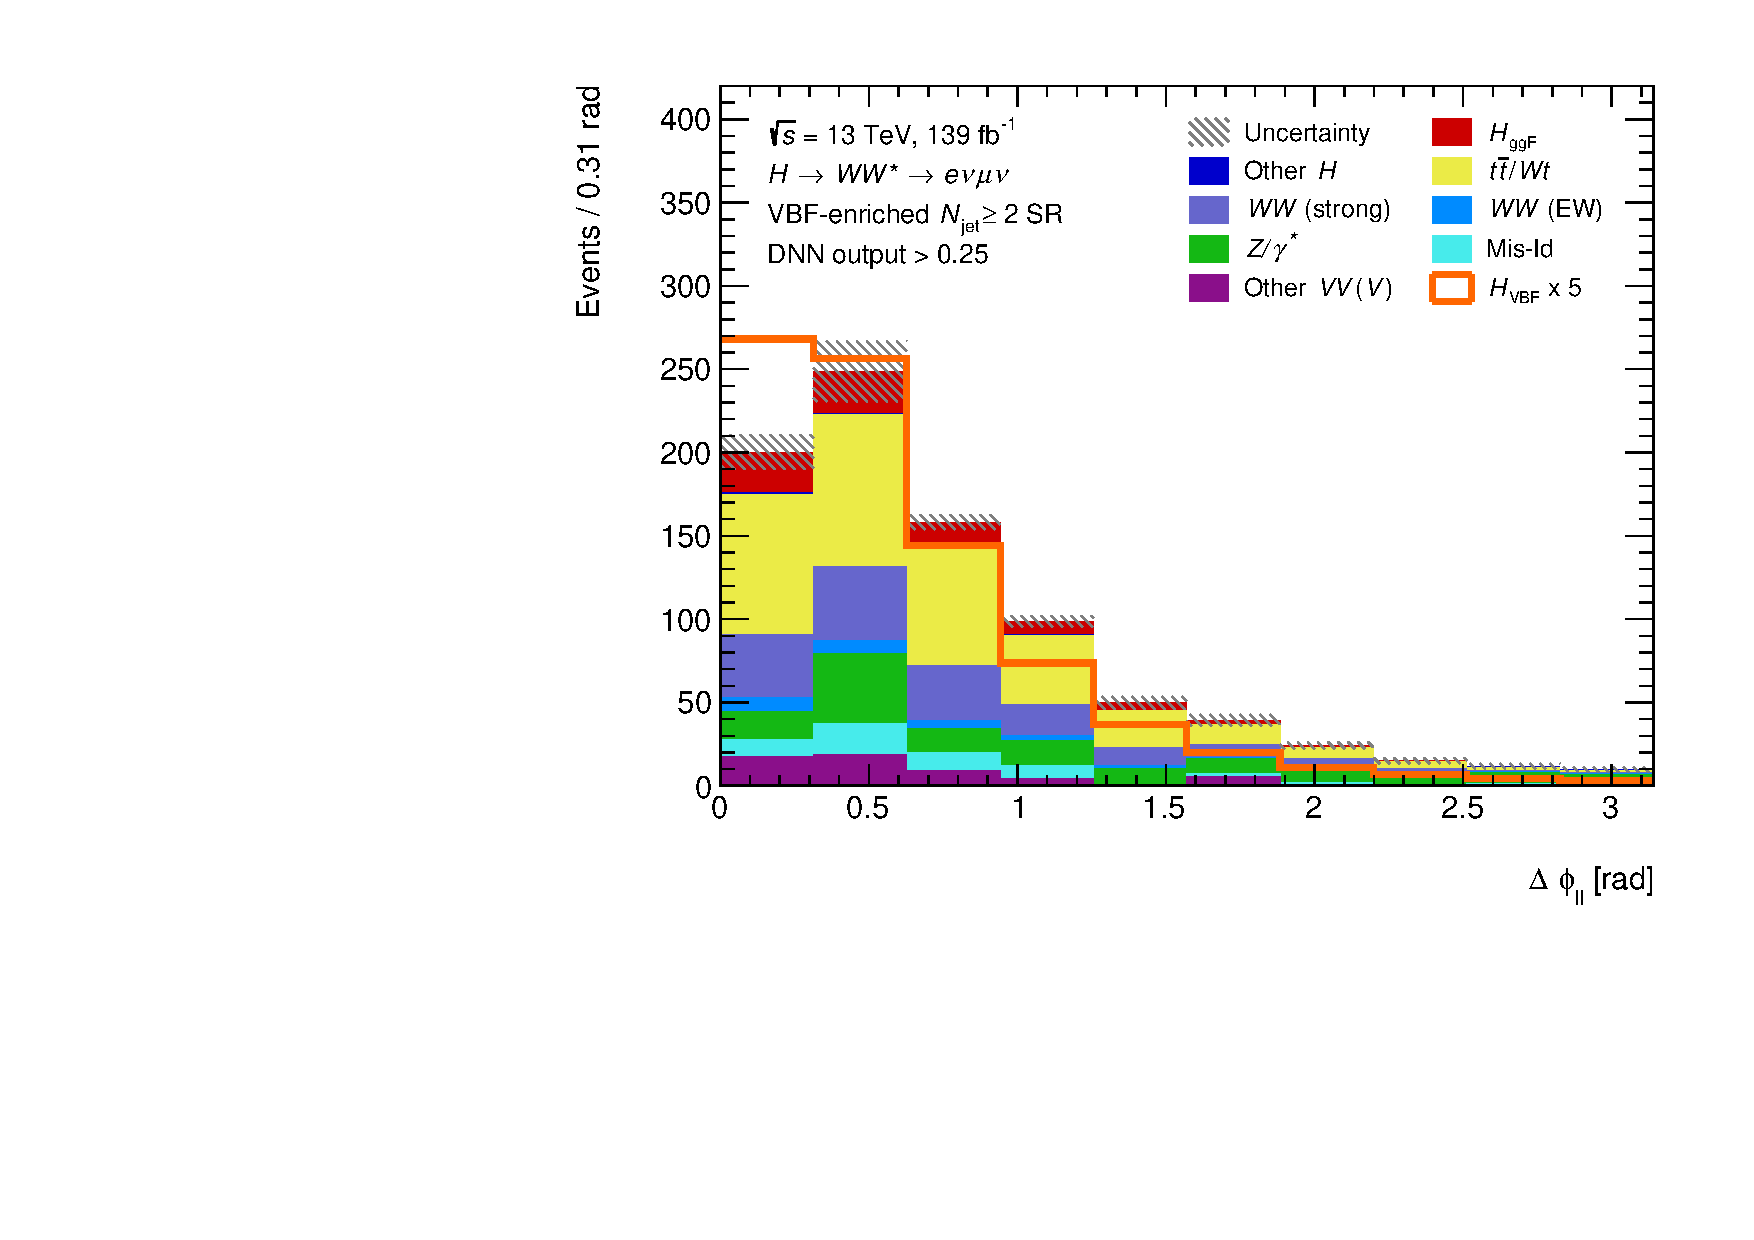
\includegraphics[width=0.32\textwidth]{figures/hww/dnn/blinded/run2-emme-CutVBFSR_DNN25-DPhill-lin.pdf} \hfill
        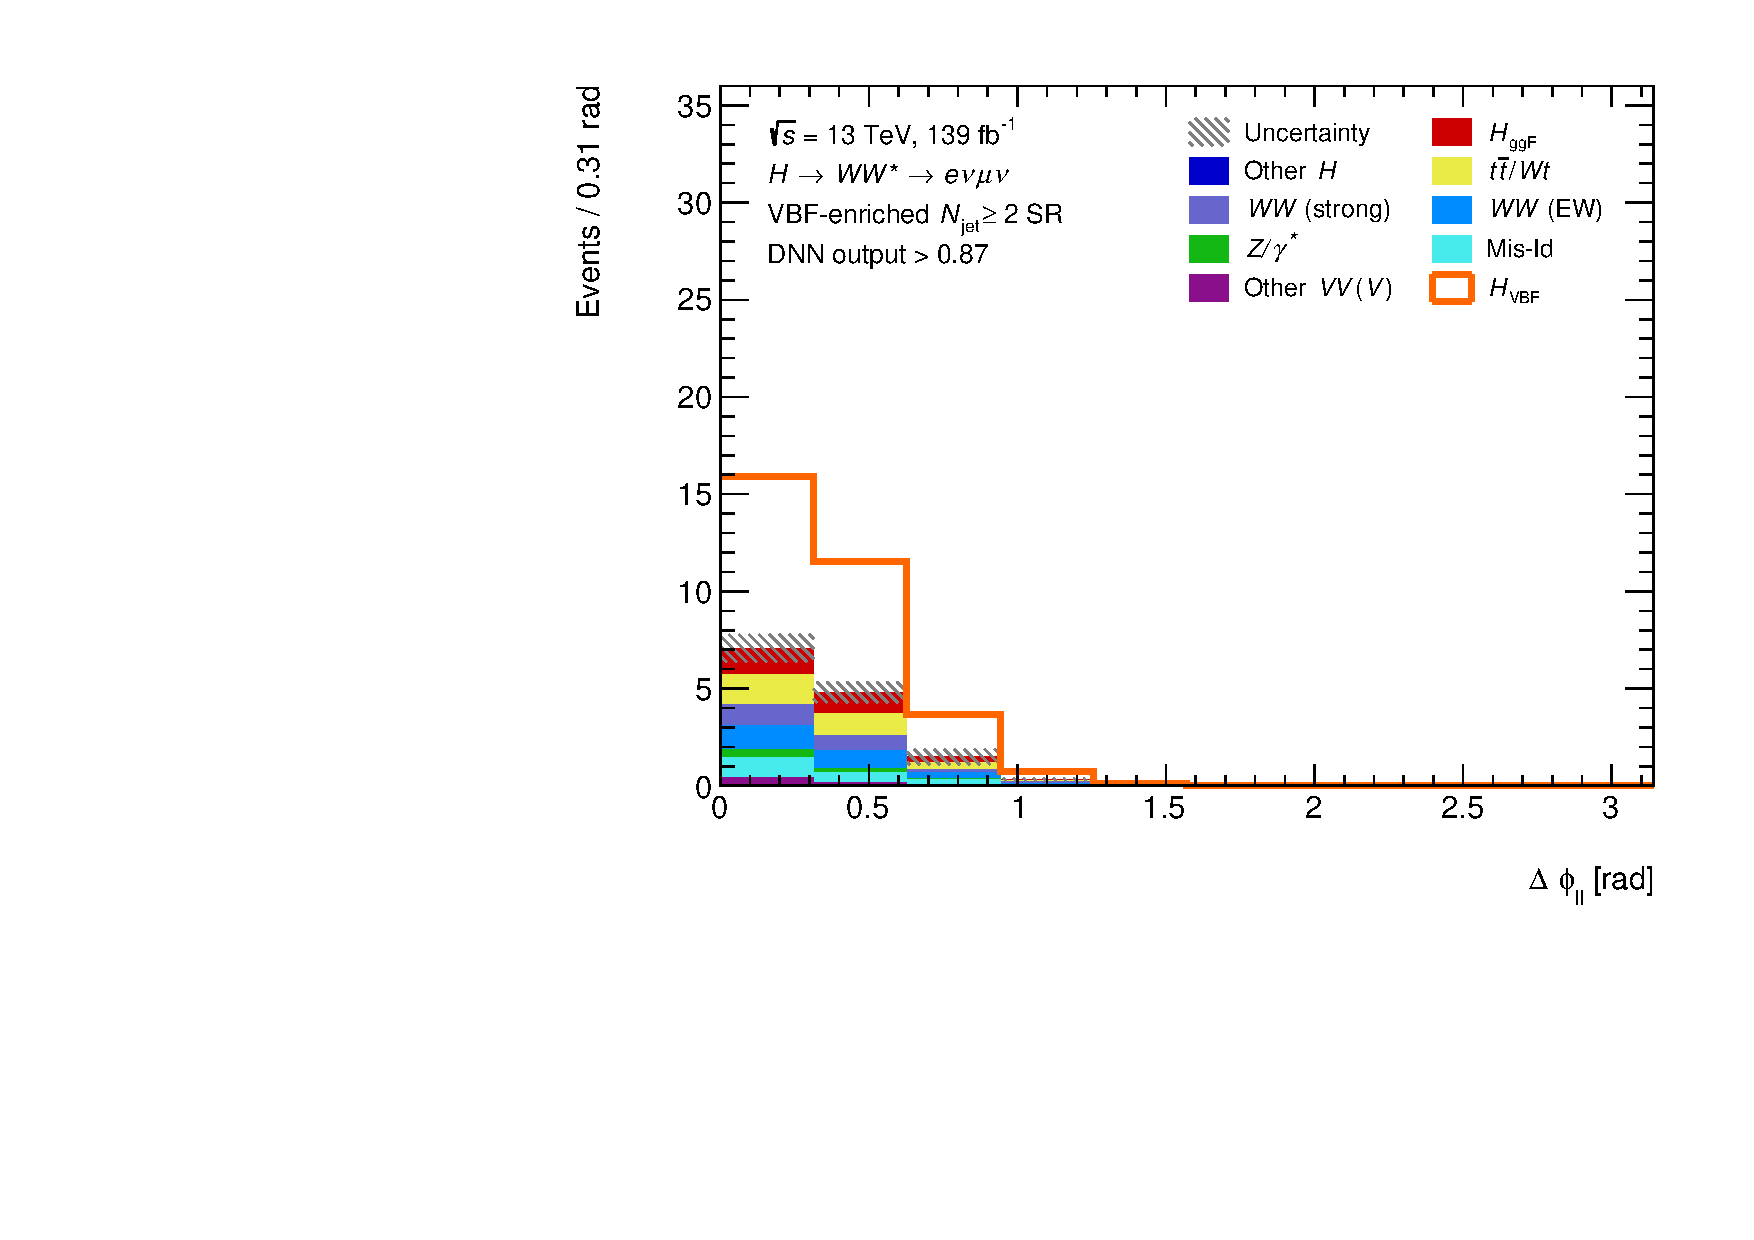
\includegraphics[width=0.32\textwidth]{figures/hww/dnn/blinded/run2-emme-CutVBFSR_DNN87-DPhill-lin.pdf}
    } \\
    \subfloat[$\mll$]{
        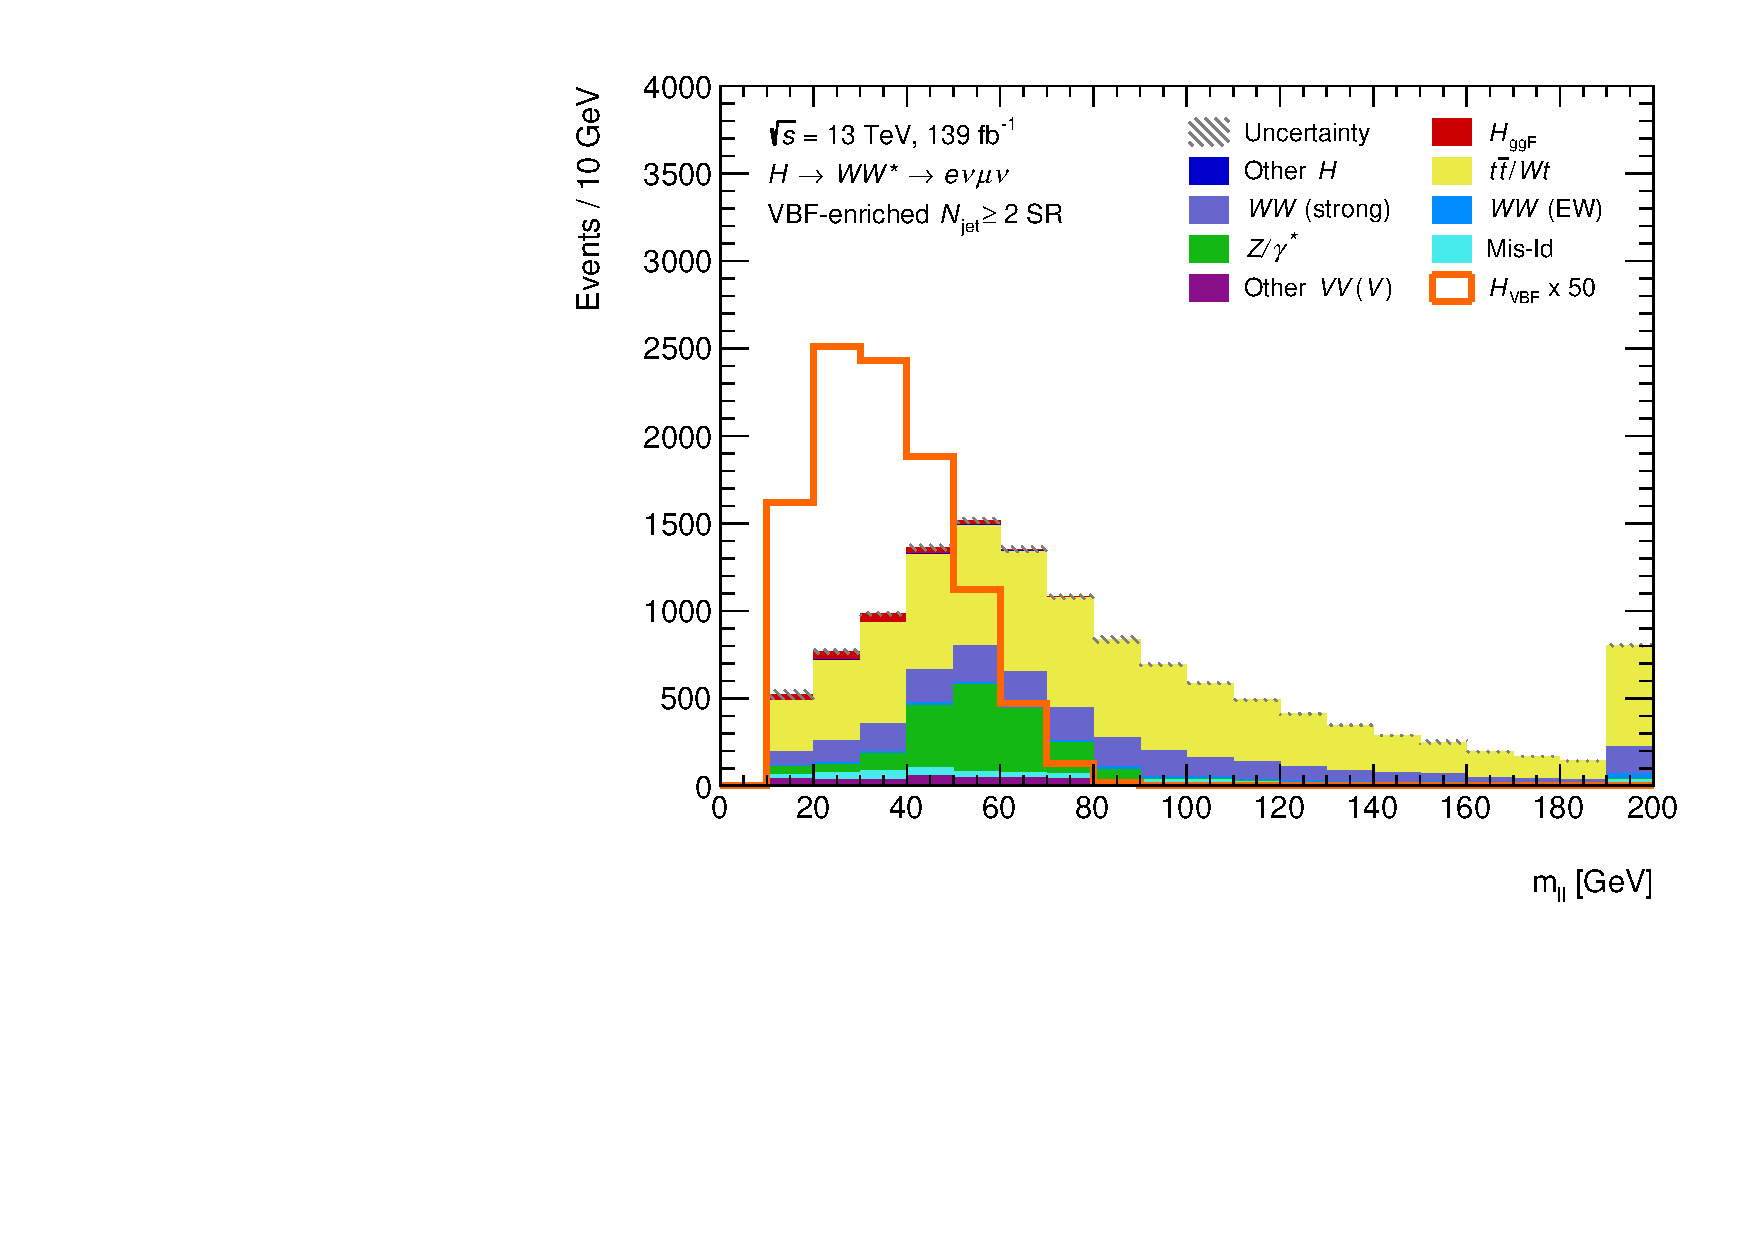
\includegraphics[width=0.32\textwidth]{figures/hww/dnn/blinded/run2-emme-CutVBF_SR-Mll-lin.pdf}
        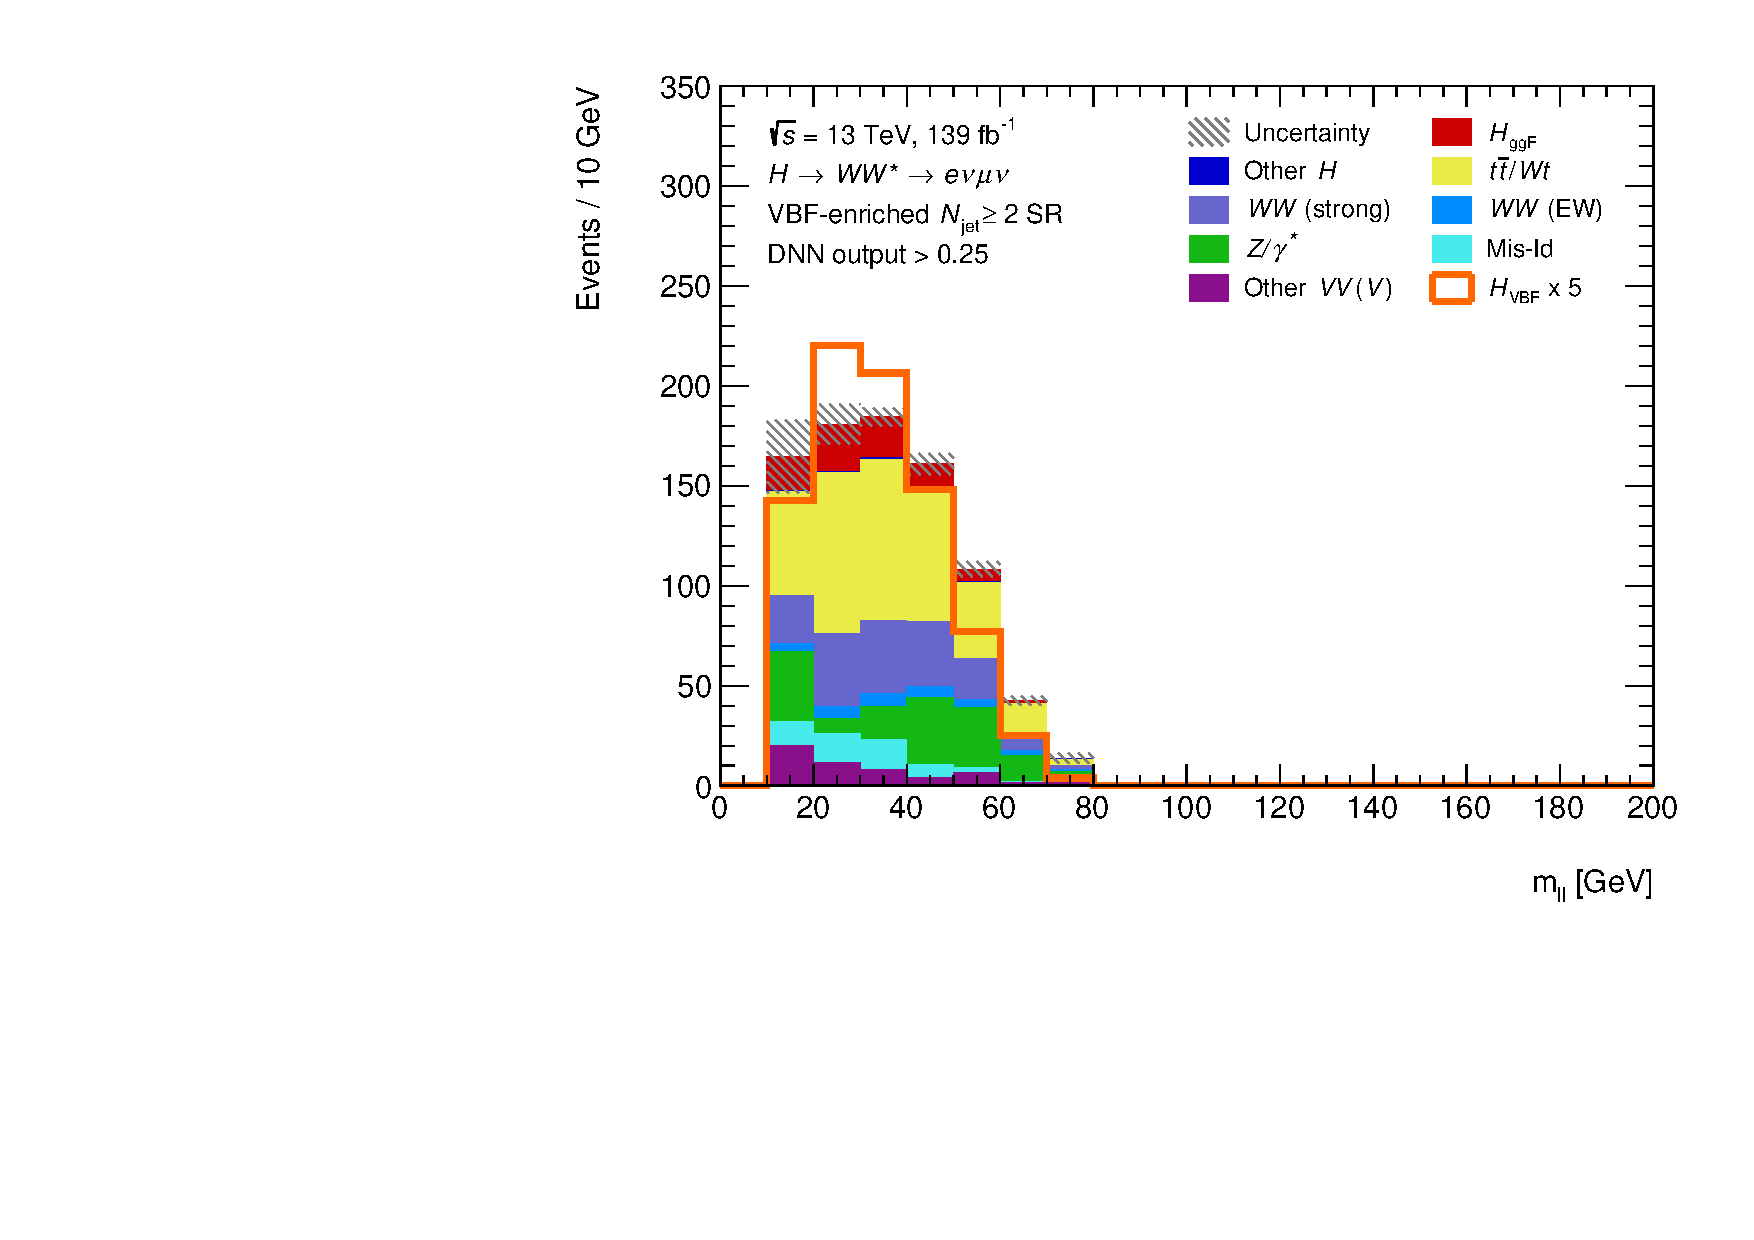
\includegraphics[width=0.32\textwidth]{figures/hww/dnn/blinded/run2-emme-CutVBFSR_DNN25-Mll-lin.pdf}
        \includegraphics[width=0.32\textwidth]{figures/hww/dnn/blinded/run2-emme-CutVBFSR_DNN87-Mll-lin.pdf}
    } \\
    \subfloat[$\mT$]{
        \includegraphics[width=0.32\textwidth]{figures/hww/dnn/blinded/run2-emme-CutVBF_SR-MT-lin.pdf} \hfill
        \includegraphics[width=0.32\textwidth]{figures/hww/dnn/blinded/run2-emme-CutVBFSR_DNN25-MT-lin.pdf} \hfill
        \includegraphics[width=0.32\textwidth]{figures/hww/dnn/blinded/run2-emme-CutVBFSR_DNN87-MT-lin.pdf}
    } 
    {\caption{Distributions of $\dphill$, $\mll$, $\mT$ in the VBF signal region.
        Each row corresponds to one variable with different selections made on the DNN output.
        \label{app:fig:dnn-inputs-hwwdecay} }}
\end{figure}



\begin{figure}[h]
    \centering
    \subfloat[$\pttot$]{
        \includegraphics[width=0.32\textwidth]{figures/hww/dnn/blinded/run2-emme-CutVBF_SR-PtTot-lin.pdf} \hfill
        \includegraphics[width=0.32\textwidth]{figures/hww/dnn/blinded/run2-emme-CutVBFSR_DNN25-PtTot-lin.pdf} \hfill
        \includegraphics[width=0.32\textwidth]{figures/hww/dnn/blinded/run2-emme-CutVBFSR_DNN87-PtTot-lin.pdf}
    } \\
    \subfloat[$\METSig$]{
        \includegraphics[width=0.32\textwidth]{figures/hww/dnn/blinded/run2-emme-CutVBF_SR-METSig_broad-lin.pdf} \hfill
        \includegraphics[width=0.32\textwidth]{figures/hww/dnn/blinded/run2-emme-CutVBFSR_DNN25-METSig_broad-lin.pdf} \hfill
        \includegraphics[width=0.32\textwidth]{figures/hww/dnn/blinded/run2-emme-CutVBFSR_DNN87-METSig_broad-lin.pdf}
    } \\
    {\caption{Distributions of $\pttot$ and $\METSig$ in the VBF signal region.
            Each row shows one variable with different cuts on the DNN output distribution being applied in different columns.
            \label{app:fig:dnn-inputs-top-sup} }}
\end{figure}
}